\chapter{AccessibleHub: Transforming mobile accessibility guidelines into code}
\label{chap:accessibility-toolkit}

\chapterintroline{
    This chapter introduces an accessibility learning toolkit for mobile developers. Building upon prior research, it provides a practical guide to implementing accessible mobile applications, particularly in Flutter. \textit{AccessibleHub}, a \gls{reactnative} toolkit, offers interactive examples and component-level guidance, comparing React Native and \gls{flutter}. Grounded in \gls{wcagg} principles, AccessibleHub aims to bridge the gap between accessibility guidelines and real-world application.
}

\section{Introduction}
\label{sec:intro}

\subsection{Challenges in implementing accessibility guidelines}

The importance of mobile app accessibility extends beyond mere compliance with legal regulations. Ensuring equal access to digital content and services is not only an ethical obligation but also a smart business decision. By prioritizing accessibility, app developers and companies can tap into a larger user base, improve user satisfaction, and demonstrate their commitment to social responsibility.
Despite the clear benefits and moral imperatives of mobile app accessibility, many developers still struggle to effectively implement accessibility guidelines in their projects. The \acrshort{wcagacr}, developed by the \gls{w3cg}, serve as the international standard for digital accessibility. However, translating these guidelines into practical implementation can be a challenging task, particularly starting from pure formal guidelines into everyday code. \\

One of the primary challenges lies in the complexity of the guidelines themselves. WCAG encompasses a wide range of \textit{success criteria}, organized under four main general \textit{principles}: perceivable, operable, understandable, and robust. Each principle contains multiple guidelines, and each guideline has several success criteria at different levels of \textit{conformance}. Navigating this intricate web of requirements and understanding how to apply them to specific mobile app components can be overwhelming for developers, especially those new to accessibility. 
Moreover, the practical implementation of accessibility guidelines often varies across different platforms and frameworks. \textit{iOS} and \textit{Android}, the two dominant mobile operating systems, have their own unique accessibility \gls{apig}s, tools, and best practices. Cross-platform frameworks like React Native and Flutter add another layer of complexity, as developers must ensure that their accessibility implementations are compatible with the underlying platform-specific mechanisms. \\ 

Furthermore, there is often a lack of clear, practical examples and guidance on how to implement accessibility features in real-world mobile app projects. While the \textit{WCAG} provides a solid foundation, it is primarily focused on web content and may not always directly address the unique challenges and interaction patterns of mobile apps. Developers often struggle to bridge the gap between the theoretical guidelines and the specific implementation details required for their projects.

\subsection{The need for practical developer education}

To address these challenges and bridge the gap between accessibility guidelines and practical implementation, there is a pressing need for developer education resources that focus on real-world, hands-on learning experiences. Traditional documentation and guidelines, while valuable, often fall short in providing the level of detail and interactivity needed to effectively guide developers through the accessibility implementation process.
This is where the concept of an \textit{accessibility learning toolkit} comes into play. An accessibility toolkit is designed to serve as a comprehensive, interactive resource that empowers developers to create accessible mobile applications by providing:

\begin{enumerate}
    \item Clear explanations of \acrshort{wcagacr} guidelines and their applicability to mobile apps;
    
    \item Step-by-step implementation guidance for common mobile app components and interaction patterns;
    
    \item Practical code examples and tutorials that demonstrate best practices;
    
    \item Hands-on exercises and challenges to reinforce learning and build confidence;
    
    \item Tools and techniques for testing and validating the accessibility of mobile apps.
\end{enumerate}

The primary goal of an accessibility learning toolkit is to bridge the gap between the theoretical knowledge of accessibility guidelines and the practical skills needed to implement them effectively in real-world projects. 
The toolkit should cater to developers at various levels of expertise, from beginners who are new to accessibility concepts to experienced professionals seeking to deepen their knowledge and stay up-to-date with the latest best practices. By providing a comprehensive, hands-on learning resource, the accessibility toolkit can play a crucial role in promoting a culture of inclusive design and development within the mobile app industry. \\

Current research, including Budai's work on Flutter accessibility testing, has primarily focused on end-user validation and testing methodologies. However, developers need practical, implementation-focused guidance that bridges multiple frameworks and platforms.
Despite widespread accessibility guidelines and standard, mobile application developers face significant challenges in translating theoretical requirements into practical implementations. This gap between guidelines and implementation is particularly evident in mobile development, where different platforms, screen sizes, and interaction models add complexity to accessibility implementation. Some of the most common challenges include:

\begin{itemize}
    \item Complex testing requirements - developers must validate across multiple devices, \gls{screenreaderg}, and interaction modes;
    
    \item Framework-specific implementations - each platform has unique accessibility \gls{apig}s and requirements;
    
    \item Limited practical examples - most documentation focuses on theoretical guidelines rather than concrete implementation patterns;
    
    \item Performance considerations - accessibility features must be implemented without compromising app performance.
\end{itemize}

Effective developer education in accessibility requires a solid grounding in learning theories that emphasize hands-on, interactive approaches. By integrating established learning theories with technical education principles, it's possible to justify the interactive and practical approach adopted in this toolkit. In doing so, we draw on constructivist and experiential learning models, which have been widely recognized as effective frameworks in technical and developer education.

Constructivist learning theories, pioneered by Piaget \cite{piaget1970science} and Vygotsky \cite{vygotsky1978mind}, posit that learning is an active process in which individuals construct knowledge based on their prior experiences and interactions with the environment. In the context of developer education, this suggests that hands-on learning is more effective than passive instruction \cite{savery2006overview}. By engaging with real-world accessibility challenges and actively experimenting with code implementations, developers can build a deeper understanding of accessibility guidelines and best practices, by having a tool at their disposal easy to use and to navigate. \\

Kolb's \textit{Experiential Learning Theory} \cite{kolb1984experiential} further supports this approach by describing learning as a four-stage cycle: concrete experience, reflective observation, abstract conceptualization, and active experimentation. For developers learning about accessibility, this cycle might involve encountering accessibility issues in their projects, analyzing existing solutions and guidelines, synthesizing their understanding of \acrshort{wcagacr} principles, and applying these principles to their own code. \textit{AccessibleHub} facilitates this learning cycle by providing a structured, interactive environment for developers to engage with accessibility concepts and implementations being organized into different core sections. By aligning with these proven pedagogical approaches, \textit{AccessibleHub} aims to provide an effective and engaging learning experience for developers. Moreover, by fostering a community of practice around accessibility while providing easier access to learning resources, this project encourages ongoing learning and knowledge sharing among developers, promoting the continuous improvement and dissemination of accessibility best practices.

\subsection{Research objectives and methodology}

Building upon previous research into mobile accessibility, this work aims to provide a comprehensive understanding of accessibility implementation across major cross-platform frameworks. While existing research indeed set grounds for both guidelines on accessibility and testing methodologies, there is a critical need to understand how these guidelines translate into practice for developers. 

This research addresses three fundamental questions about accessibility implementation in mobile development frameworks (referring to these ones as \textit{research questions}, following the work in \cite{perinello2024accessibility}:

\begin{itemize}
    \item First, we investigate whether components and widgets provided by frameworks are \textit{accessible by default}, without requiring additional developer intervention. This analysis is crucial for understanding the baseline accessibility support provided by each framework and identifying areas where additional implementation effort may be required;
    
    \item Second, we examine the \textit{feasibility of making non-accessible components accessible} through additional development effort. This involves analyzing the technical capabilities of each framework and identifying the necessary modifications to achieve accessibility compliance;
    
    \item Third, we quantify the \textit{development overhead required to implement accessibility features} when they are not provided by default. This includes measuring additional code requirements, analyzing complexity increases, and evaluating the impact on development workflows.
\end{itemize}

These questions is addressed via the usage of a systematic methodology aiming to address in detail accessibility support in React Native and Flutter, focusing on component implementation patterns and native platform integration. The implementation is comparative, allowing developers to directly implement accessible code examples with different degrees of implementation complexity measured quantitatively (including lines of code, required properties, and additional components needed for accessibility support). Comprehensive testing of implementations is also done using screen readers and other assistive technologies to verify accessibility compliance.

The \textit{goal} is to create an accessible application that serves three key purposes:
\begin{enumerate}
    \item To provide developers with practical, interactive examples of accessibility implementation, able to be copied easily and ported inside of other projects;
    
    \item To compare and contrast accessibility approaches between the main cross-development mobile frameworks in the current mobile landscape;
    
    \item To establish a reusable pattern library that demonstrates engine architecture, widget systems, and native platform integration, while ensuring compliance with current accessibility guidelines and legal requirements.
\end{enumerate}

The following sections will detail the development of \textit{AccessibleHub}, an application developed in React Native designed to serve as a practical manual for implementing accessibility features. While the technical aspects of cross-platform frameworks will be discussed later, the focus remains on providing developers with actionable implementation patterns and comparative insights for building accessible applications.

\section{React Native Overview}
\label{sec:reactnative-overview}

\gls{reactnative} is an open-source framework developed by Meta that enables developers to build mobile applications using \textit{JavaScript} and the \textit{React} paradigm (\cite{site:reactnative}). It employs a declarative, component-based approach through the use of \textit{JSX}, which is an XML-like syntax that allows developers to intermix \textit{JavaScript} logic with markup. This combination not only improves code readability but also enhances modularity and facilitates code reuse.

\begin{figure}[ht]
    \centering
    
\includegraphics[width=0.4\textwidth, alt={React Native logo}]{img/react-native-logo.png}
    \caption{React Native logo}
\label{fig:reactnative-logo}
\end{figure}

\subsection{Core architecture and features}
\begin{itemize}
    \item \textit{Component-based architecture:}  
    The entire user interface in React Native is built from reusable components. Each component encapsulates its own logic and presentation, which greatly aids in the maintainability and scalability of complex applications;
    
    \item \textit{JSX syntax:}  
    Developers write the \acrshort{ui} using \textit{JSX}, a syntax extension similar to \textit{HTML}. This blending of code and layout simplifies the development process and enables a more intuitive understanding of the component structure;
    
    \item \textit{Bridging mechanism:}  
    React Native’s bridge enables asynchronous communication between the \textit{JavaScript} layer and native modules. This means that while the application is written in \textit{JavaScript}, performance-critical tasks can be executed using native code (e.g., \textit{Objective-C, Swift}, or \textit{Java}), ensuring a native look and feel without sacrificing performance;
    
    \item \textit{Hot reloading:}  
    One of the standout features present in this framework, which allows developers to see changes in real time without restarting the entire application. This accelerates the development cycle and aids in rapid prototyping;
    
    \item \textit{Unified codebase:}  
    React Native enables the development of applications for both iOS and Android using a single codebase. This unified approach reduces development time and effort compared to maintaining separate codebases for each platform.
\end{itemize}

\subsection{Accessibility in React Native}
React Native provides a robust set of accessibility features that are deeply integrated into its component model. This allows developers to create inclusive applications without relying on external libraries or writing platform-specific code (following what's present into \cite{site:reactnativeaccess}). Here are the key accessibility features in React Native:

\begin{itemize}
    \item \textbf{Accessibility properties}: React Native components can be enhanced with a variety of accessibility properties that provide semantic meaning and context for assistive technologies. These properties include:
    \begin{itemize}
        \item \texttt{accessibilityLabel}: A concise, descriptive string that identifies the component for screen reader users;
        \item \texttt{accessibilityRole}: Defines the component's semantic role (e.g., \texttt{"button"}, \texttt{"header"}), helping assistive technologies interpret its purpose correctly;
        \item \texttt{accessibilityHint}: Provides additional context about a component's function or the result of interacting with it;
        \item \texttt{accessibilityState}: Describes the current state of a component (e.g., \texttt{selected}, \texttt{disabled}), which is essential for conveying dynamic changes.
    \end{itemize}
    
    \item \textbf{Accessibility actions}: React Native allows developers to define custom accessibility actions for components, enabling advanced interactions beyond the default gestures. For example, a custom \texttt{accessibilityAction} could be added to a component to trigger a specific behavior when activated by an assistive technology;
    
    \item \textbf{Accessibility focus}: React Native manages accessibility focus automatically, ensuring that the correct component receives focus when navigating with assistive technologies. Developers can also programmatically control focus using the \\ \texttt{accessibilityElementsHidden} and \\\texttt{importantForAccessibility} properties;
    
    \item \textbf{Accessibility events}: React Native provides accessibility events that notify assistive technologies when important changes occur in the application. These events include:
    \begin{itemize}
        \item \texttt{onAccessibilityTap}: Called when a user double-taps a component while using an assistive technology;
        \item \texttt{onMagicTap}: Called when a user performs the "magic tap" gesture (a double-tap with two fingers) to activate a component;
        \item \texttt{onAccessibilityFocus}: Called when a component receives accessibility focus;
        \item \texttt{onAccessibilityBlur}: Called when a component loses accessibility focus.
    \end{itemize}
\end{itemize}

By leveraging these built-in accessibility features, developers can create React Native applications that are inclusive and accessible to users with diverse needs and abilities. The tight integration of accessibility into the core component model ensures that developers can create accessible apps without sacrificing performance or maintainability.

\subsection{Advantages and developer benefits}

Using React Native offers several benefits for developers, briefly listed here:
\begin{itemize}
    \item \textit{Rapid development:}  
    Thanks to hot reloading and a vast ecosystem of reusable components, developers can iterate quickly and efficiently;
    
    \item \textit{Cross-platform consistency:}  
    With a unified codebase for both iOS and Android, developers can ensure a consistent user experience without duplicating effort;
    
    \item \textit{Integrated accessibility:}  
    React Native’s direct integration of accessibility properties allows developers to implement accessible features without having to rely on external tools or write platform-specific code;
    
    \item \textit{Community and support:}  
    A large and active community means extensive documentation, a wealth of third-party libraries, and a robust support network for troubleshooting and enhancements;
    
    \item \textit{Seamless transition for web developers:}  
    Developers familiar with React for web applications will find the transition to React Native smooth, as the core concepts and \textit{JSX} syntax remain consistent.
\end{itemize}

\subsection{Differences from native iOS/Android and web development}
\begin{itemize}
    \item \textit{Native iOS/Android:}  
    In native development, accessibility is handled through platform-specific \gls{apig}: \gls{voiceover} on \textit{iOS} and \gls{talkback} on \textit{Android}, which require different tools and approaches. React Native provides a unified \textit{API}s, streamlining the implementation of accessibility features across both platforms.
    
    \item \textit{Web development:}  
    Whereas web accessibility is achieved by adding \gls{ariag} attributes to \textit{HTML}, React Native integrates accessibility directly within its component structure. This intrinsic approach treats accessibility as a core attribute of each component, rather than an external addition.
\end{itemize}

In summary, React Native offers a modern, efficient, and developer-friendly environment that not only simplifies cross-platform mobile development but also incorporates accessibility into its core design. This makes it an ideal choice for creating inclusive applications, and it forms the foundational platform upon which the \textit{AccessibleHub} toolkit is built.

\section{AccessibleHub: An Interactive Learning Toolkit}
\label{sec:accessiblehub}

\subsection{Core architecture and design principles}
\label{sec:accessiblehub-architecture-design}

\textit{AccessibleHub} is a React Native application designed to serve as an interactive manual for implementing accessibility features in mobile development. Unlike traditional documentation or testing frameworks, the application provides developers with hands-on examples and implementation patterns that can be directly applied to their projects.

The application is structured around four conceptual main sections:
\begin{enumerate}
    \item \textit{Component examples}: Interactive demonstrations of common \acrshort{ui} elements with proper accessibility implementations, including buttons, forms, media content, and navigation patterns. This allows developers to clearly see the implementation of an accessible component and easily copy the code to their convenience;
    
    \item \textit{Framework comparison}: A detailed analysis of accessibility implementation approaches between React Native and Flutter, highlighting differences in component structure, properties, and required code;
    
    \item \textit{Testing tools}: Built-in utilities for validating accessibility features, allowing developers to understand how screen readers and other assistive technologies interact with their implementations;
    
    \item \textit{Implementation guidelines}: Technical documentation that connects WCAG requirements to practical code examples, providing clear paths for meeting accessibility standards.
\end{enumerate}

Each component presented serves dual purposes: demonstrating proper accessibility implementation while providing reusable code patterns. The application emphasizes practical implementation over theoretical guidelines, showing developers not just what to implement effectively. By focusing on developer experience, \textit{AccessibleHub} bridges the gap between accessibility requirements and actual implementation, providing a resource that can be directly integrated into the development workflow. \\

The \textit{design} philosophy of \textit{AccessibleHub} is founded on principles that bridge theoretical accessibility guidelines with practical implementation needs. While analyzing the current landscape of mobile development frameworks and accessibility implementation presented in \ref{chap:accessibility-literature}, a clear pattern emerges: developers need more practical, implementation-focused guidance that directly addresses the complexity of building accessible applications. To address this need, \textit{AccessibleHub} adopts three fundamental architectural principles:

\begin{enumerate}
    \item The usage of a \textit{component-first architecture}, where each UI element exists as an independent, self-contained unit demonstrating both implementation patterns and accessibility features. In other words, each one of them is being constructed within an \textit{accessibility-first} experience which ensures that usage of screen readers and other assistive technologies is kept as a priority. This modular approach provides two advantages: it first allows developers to comprehend and apply accessibility features in isolation, hence reducing cognitive load and implementation complexity, and enables systematic testing and validation of accessibility features of every component. Also, this means accessibility patterns can be studied, implemented, and verified in isolation from added complexity brought in by interactions among those components;

    \item \textit{Progressive enhancement} as a core design methodology. Instead of presenting accessibility as big challenge from the start, components are structured in increasing levels of complexity. This starts with basic elements like buttons and text inputs where basic accessibility patterns can be established. As developers master these foundational components, the application introduces more complex patterns such as forms, navigation systems, and gesture-based interactions. This helps into guiding the development towards more complicated scenarios;

    \item Focus on \textit{framework-agnostic patterns}, not depending on a specific framework while providing concrete code implementations. Even though \textit{AccessibleHub} has been implemented in React Native, all the patterns and principles explained are designed to transcend into specific framework implementations. The approach wants to give importance to the compatibility and reusability in the framework on the mobile development side. It will compare the implementations, mainly between React Native and Flutter, to show how developers can port accessibility patterns across different frameworks and understand core accessibility concepts in an easy-to-implement manner within professional projects. 
    
\end{enumerate}

Through these principles, \textit{AccessibleHub} aims to transform accessibility from an afterthought into an \textit{accessibility-by-design}. The application serves not just as a reference implementation, but as an educational tool that guides developers through the process of building truly accessible applications. This approach recognizes that effective accessibility implementation requires both theoretical understanding and practical experience, providing developers with the tools they need to create more inclusive mobile applications.

\subsection{Educational framework design}
\label{sec:accessiblehub-educational-framework}

\textit{AccessibleHub}'s educational framework is designed to provide a structured, incremental learning experience that progressively builds accessibility knowledge and skills. The content is organized into different \textit{learning modules}, each focusing on a key aspect of mobile accessibility. This is structured incrementally, so to help a developer gather a general idea on what needs to be implemented following a practical roadmap of steps: this allows to focus on different aspects of mobile accessibility, selecting each time the most relevant ones.

The core of the application is divided into different main screens, following:

\begin{enumerate}
    \item \textbf{Home} - The entry point for the \textit{AccessibleHub} application (\ref{fig:homescreen}). It provides an overview of the main sections and guides users on where to start their accessibility learning journey. The Home screen is designed to be intuitive and user-friendly, with clear call-to-action towards the accessible components section, allowing a developer or a user navigate to the desired section from the Home screen, comprehensive of comparison between the main mobile frameworks, learn about best practices in mobile accessibility and access testing tools documentation. There is also present a compliance dashboard provides an overview of an app's accessibility compliance status, based on the \acrshort{wcagacr} and \acrshort{mcagacr} guidelines. Developers can use this information to prioritize their accessibility efforts and focus on the areas that need the most attention;

    \begin{figure}[ht]
    \centering
    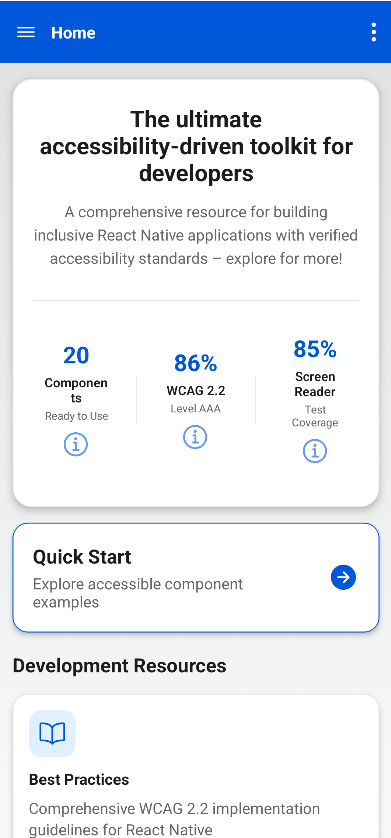
\includegraphics[width=0.4\linewidth, alt={Screenshot of the Home screen of AccessibleHub}]{img/homescreen.png}
    \caption{The Home screen of \textit{AccessibleHub}}\label{fig:homescreen}
    \end{figure}

\pagebreak

    \item \textbf{Accessible Components} - The Components section embodies a progressive learning pathway, beginning with fundamental elements (buttons, forms) before advancing to complex patterns (dialogs, advanced controls). Each component demonstrates implementation patterns through three integrated learning elements: interactive examples, annotated code, and explicit connections to relevant WCAG criteria, creating a complete educational cycle. (\ref{fig:components}). 

    \begin{figure}[ht]
    \centering
    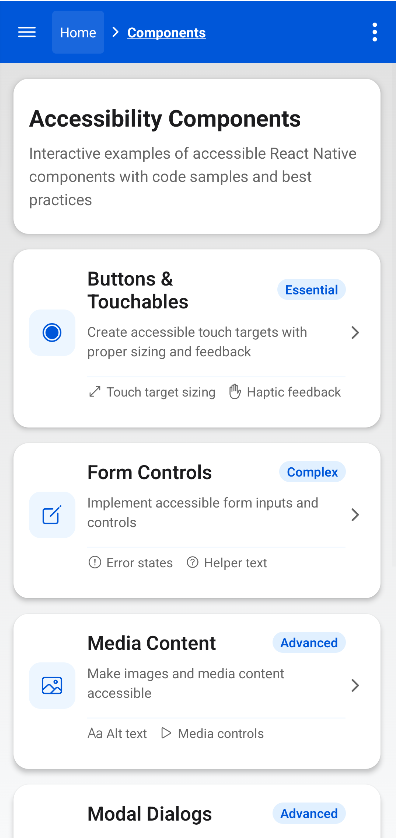
\includegraphics[width=0.4\linewidth, alt={Screenshot of the Components screen of AccessibleHub}]{img/components.png}
    \caption{The Components screen of \textit{AccessibleHub}}\label{fig:components}
    \end{figure}
    
    \pagebreak
    
    Throughout the Components section, code implementations are shared as examples, which developers can easily copy to their clipboard and integrate into their own projects. This hands-on approach allows developers to quickly apply the accessibility principles they learn and see the results in action.
    It is divided into four subscreens, each focusing on a specific category of components:

    \begin{itemize}
        \item \textit{Buttons and Touchables}: It covers the implementation of accessible buttons and touchable elements (\ref{fig:button_screens_sidebyside}). It provides code examples and best practices for ensuring that these interactive elements are perceivable, operable, and understandable by all users, including those with disabilities;

        \begin{figure}[ht]
            \centering
            \begin{subfigure}[b]{0.48\textwidth}
                \centering
                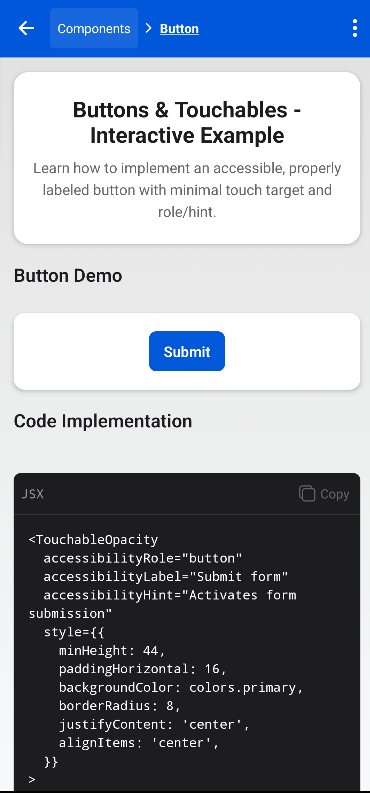
\includegraphics[width=\linewidth, alt={First part of the Buttons and touchables screen}]{img/button1.png}
                \caption{Button screen - Part 1}
                \label{fig:button-left}
            \end{subfigure}
            \hfill
            \begin{subfigure}[b]{0.48\textwidth}
                \centering
                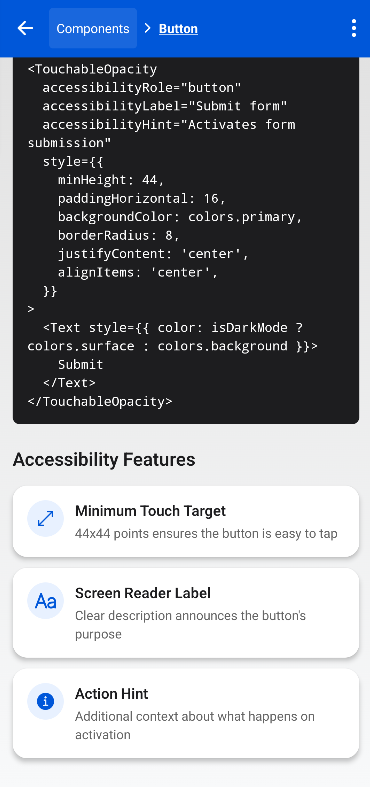
\includegraphics[width=\linewidth, alt={Second part of the Buttons and touchables screen}]{img/button2.png}
                \caption{Button screen - Part 2}
                \label{fig:button-right}
            \end{subfigure}
            \caption{Side-by-side view of the two Button and Touchables screen parts}
            \label{fig:button_screens_sidebyside}
        \end{figure}

        \FloatBarrier

        \item \textit{Forms}: The subscreen focuses on creating accessible input forms, including text fields, checkboxes, radio buttons, and date/time pickers (\ref{fig:form_screens_sidebyside}). It demonstrates how to properly label form elements, provide instructions and feedback, and ensure that forms can be navigated and completed using various input methods, such as keyboards and screen readers;

        \begin{figure}[ht]
            \centering
            \begin{subfigure}[b]{0.48\textwidth}
                \centering
                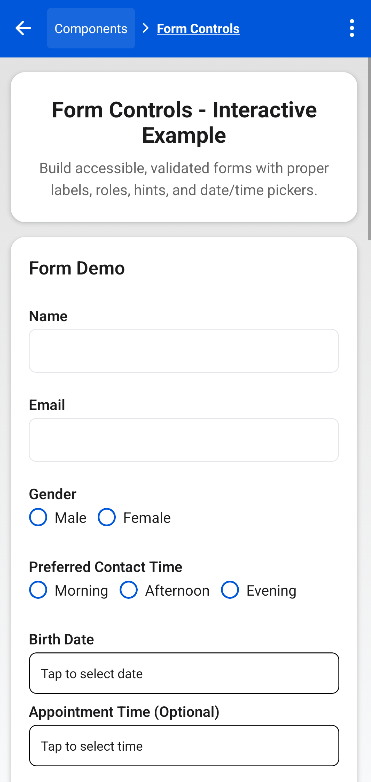
\includegraphics[width=\linewidth, alt={First part of the Form creen}]{img/form1.png}
                \caption{Form screen - Part 1}
                \label{fig:form-left}
            \end{subfigure}
            \hfill
            \begin{subfigure}[b]{0.48\textwidth}
                \centering
                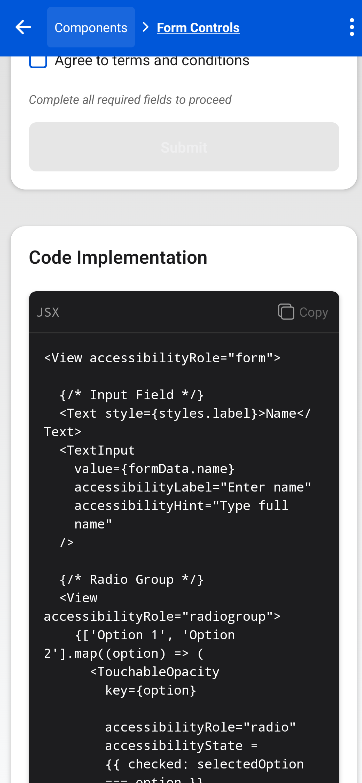
\includegraphics[width=\linewidth, alt={Second part of the Form screen}]{img/form2.png}
                \caption{Form screen - Part 2}
                \label{fig:form-right}
            \end{subfigure}
            \caption{Side-by-side view of the two Form screen parts}
            \label{fig:form_screens_sidebyside}
        \end{figure}

        \item \textit{Media}: In the Media subscreen, developers learn how to make media content, such as images, videos, and audio, accessible to users with visual or auditory impairments (\ref{fig:media_screens_sidebyside}). This includes providing alternative text for images, captions for videos, and transcripts for audio content;

        \begin{figure}[ht]
            \centering
            \begin{subfigure}[b]{0.48\textwidth}
                \centering
                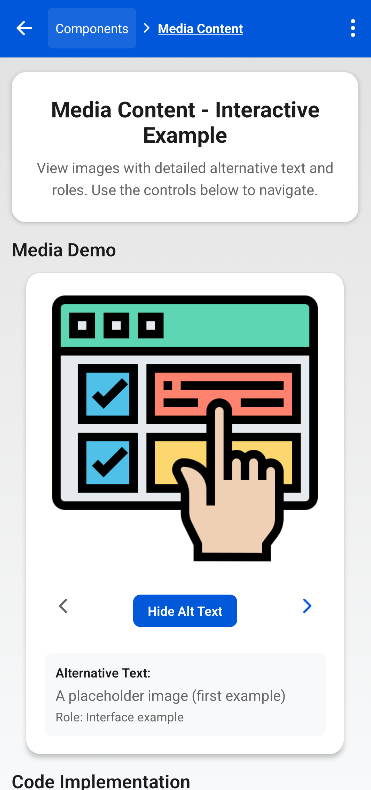
\includegraphics[width=\linewidth, alt={First part of the Media screen}]{img/media1.png}
                \caption{Media screen - Part 1}
                \label{fig:media-left}
            \end{subfigure}
            \hfill
            \begin{subfigure}[b]{0.48\textwidth}
                \centering
                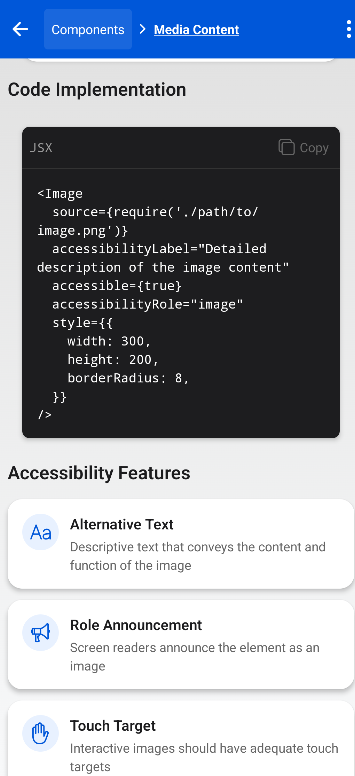
\includegraphics[width=\linewidth, alt={Second part of the Media screen}]{img/media2.png}
                \caption{Media screen - Part 2}
                \label{fig:media-right}
            \end{subfigure}
            \caption{Side-by-side view of the two Media screen parts}
            \label{fig:media_screens_sidebyside}
        \end{figure}

        \item \textit{Dialogs}: It covers the creation of accessible modal dialogs, popups, and alerts (\ref{fig:dialog_screens_sidebyside}). It provides guidance on how to ensure that these elements are properly announced by screen readers, can be easily dismissed, and do not interfere with the user's ability to navigate the application, maintaining focus management and ensuring clear exit strategies;

        \begin{figure}[ht]
            \centering
            \begin{subfigure}[b]{0.48\textwidth}
                \centering
                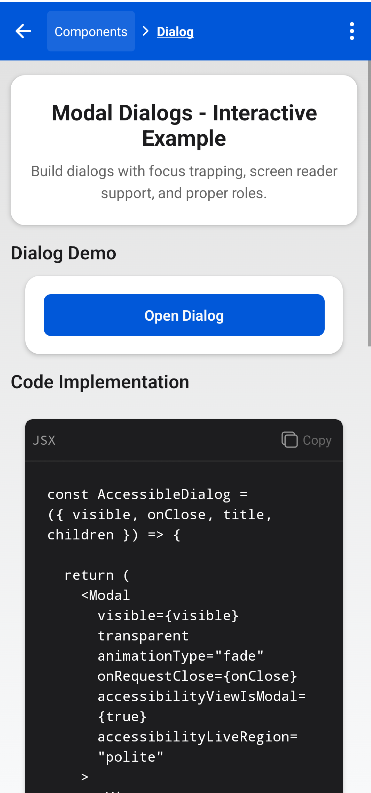
\includegraphics[width=\linewidth, alt={First part of the Dialog screen}]{img/dialog1.png}
                \caption{Dialog screen - Part 1}
                \label{fig:dialog-left}
            \end{subfigure}
            \hfill
            \begin{subfigure}[b]{0.48\textwidth}
                \centering
                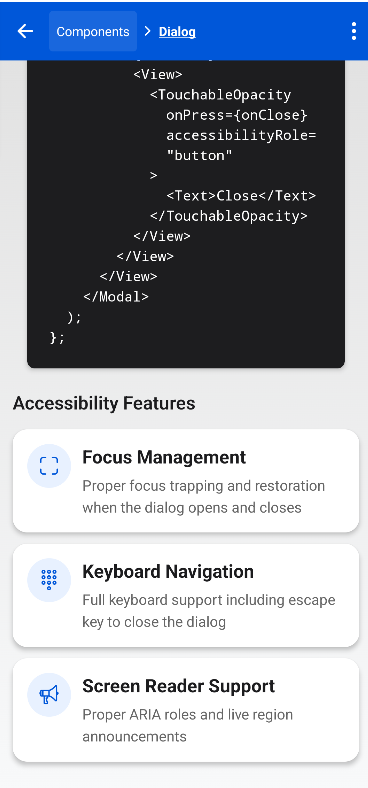
\includegraphics[width=\linewidth, alt={Second part of the Dialog screen}]{img/dialog2.png}
                \caption{Dialog screen - Part 2}
                \label{fig:dialog-right}
            \end{subfigure}
            \caption{Side-by-side view of the two Dialog screen parts}
            \label{fig:dialog_screens_sidebyside}
        \end{figure}

       \item \textit{Advanced}: This particular subscreen covers elements like alerts, sliders, progress bars and tab navigation, analyzing how accessibility may regard different animated or interactive components for more complex gesture interactions used everyday by users (\ref{fig:advanced_screens_sidebyside1} and \ref{fig:advanced_screens_sidebyside2}).

       \begin{figure}[ht]
            \centering
            \begin{subfigure}[b]{0.48\textwidth}
                \centering
                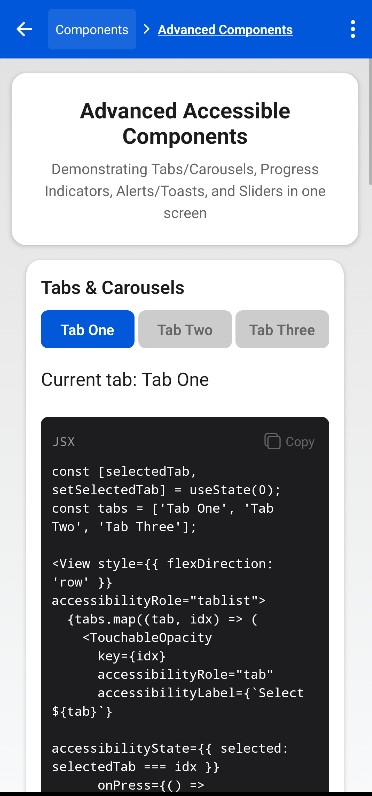
\includegraphics[width=\linewidth, alt={First part of the Advanced screen}]{img/advanced1.png}
                \caption{Advanced screen - Part 1}
                \label{fig:advanced-left1}
            \end{subfigure}
            \hfill
            \begin{subfigure}[b]{0.48\textwidth}
                \centering
                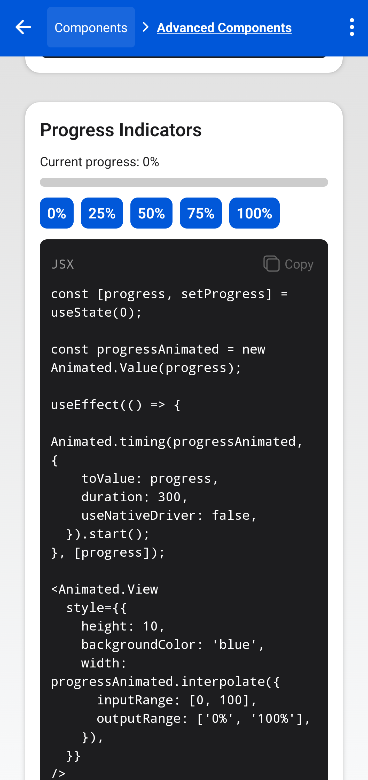
\includegraphics[width=\linewidth, alt={Second part of the Advanced screen}]{img/advanced2.png}
                \caption{Advanced screen - Part 2}
                \label{fig:advanced-right1}
            \end{subfigure}
            \caption{Side-by-side view of the first two Advanced screen parts}
            \label{fig:advanced_screens_sidebyside1}
        \end{figure}

        \begin{figure}[ht]
            \centering
            \begin{subfigure}[b]{0.48\textwidth}
                \centering
                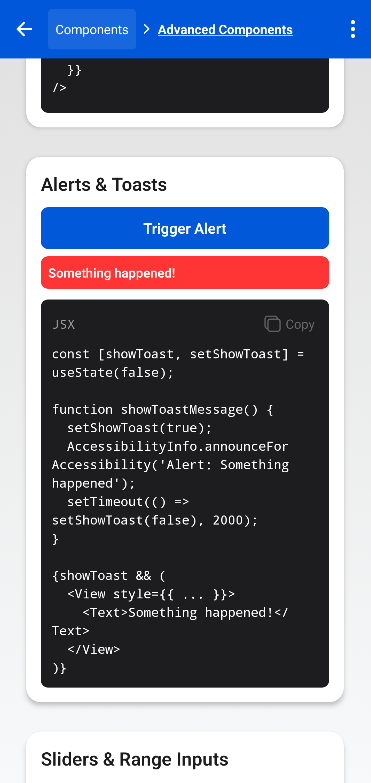
\includegraphics[width=\linewidth, alt={Third part of the Advanced screen}]{img/advanced3.png}
                \caption{Advanced screen - Part 3}
                \label{fig:advanced-left2}
            \end{subfigure}
            \hfill
            \begin{subfigure}[b]{0.48\textwidth}
                \centering
                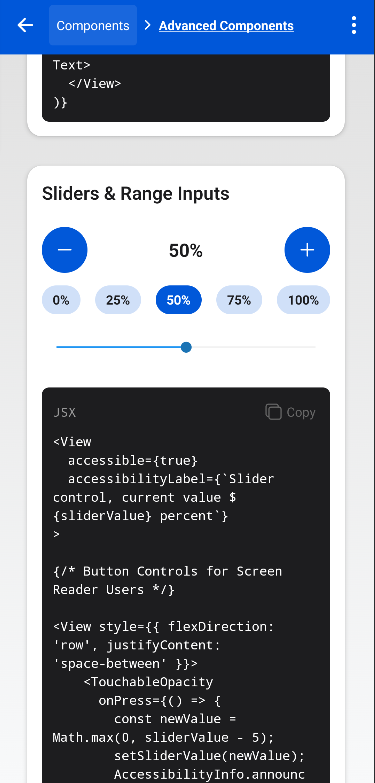
\includegraphics[width=\linewidth, alt={Fourth part of the Advanced screen}]{img/advanced4.png}
                \caption{Advanced screen - Part 4}
                \label{fig:advanced-right2}
            \end{subfigure}
            \caption{Side-by-side view of the second two Advanced screen parts}
            \label{fig:advanced_screens_sidebyside2}
        \end{figure}

    \FloatBarrier
        
    \end{itemize}

\item \textbf{Best Practices} - This section implements a conceptual learning pathway that organizes accessibility knowledge into cognitive domains rather than technical implementations. Each practice area utilizes visual encoding through color and iconography to reinforce conceptual boundaries, while badges differentiate learning modalities (documentation, code examples and guides) to accommodate diverse learning styles (\ref{fig:best-practices}).

\begin{figure}[ht]
\centering
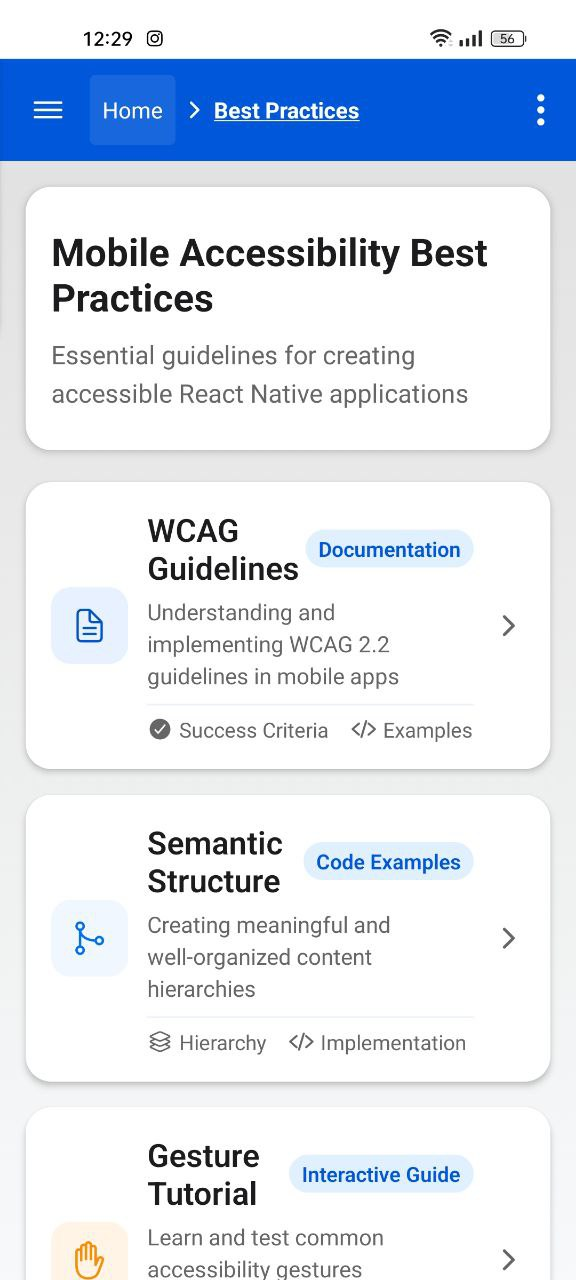
\includegraphics[width=0.4\linewidth, alt={Screenshot of the Best Practices screen of AccessibleHub}]{img/best-practices.jpg}
\caption{The Best Practices screen of \textit{AccessibleHub}}\label{fig:best-practices}
\end{figure}

\pagebreak

It is divided into five subscreens, each addressing a key aspect of mobile accessibility:

    \begin{itemize}
        \item \textit{Gestures Tutorial}: This subscreen provides an overview of the various gesture interactions used in mobile applications and how to make them accessible to users with motor impairments or those relying on assistive technologies (\ref{fig:gestures_screens_sidebyside}). It covers best practices for implementing alternative input methods and providing clear instructions and feedback. These gestures are general, tested to be used universally, both by everyday users and screen reader ones;

        \begin{figure}[ht]
            \centering
            \begin{subfigure}[b]{0.48\textwidth}
                \centering
                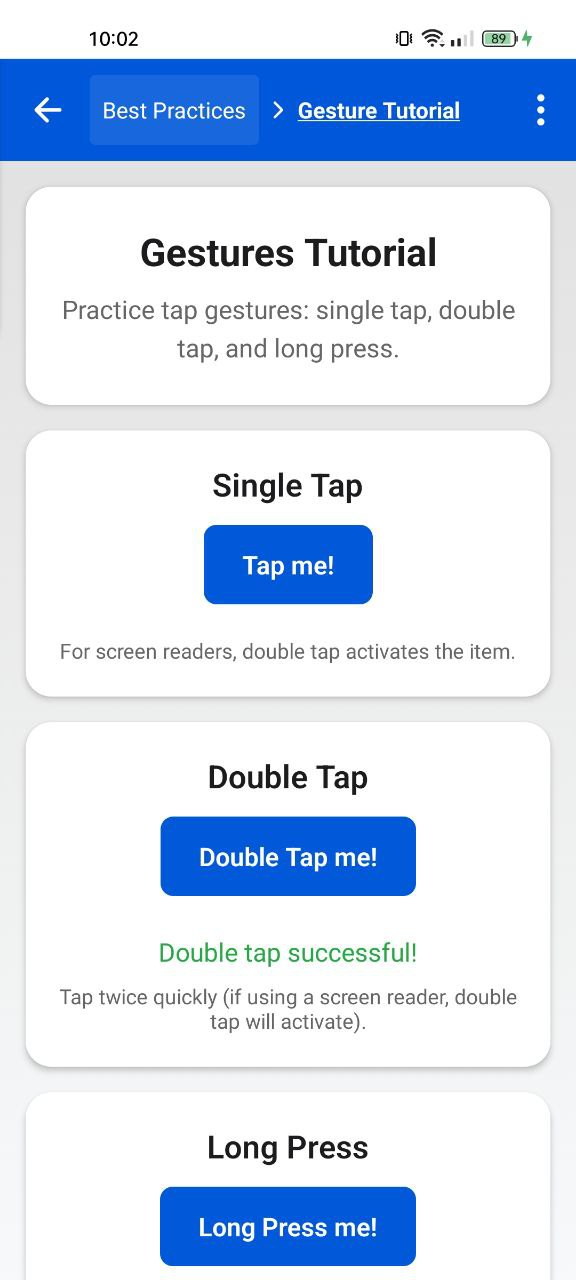
\includegraphics[width=\linewidth, alt={First part of the Gestures tutorial screen}]{img/gestures1.jpg}
                \caption{Gestures tutorial screen - Part 1}
                \label{fig:gestures-left}
            \end{subfigure}
            \hfill
            \begin{subfigure}[b]{0.48\textwidth}
                \centering
                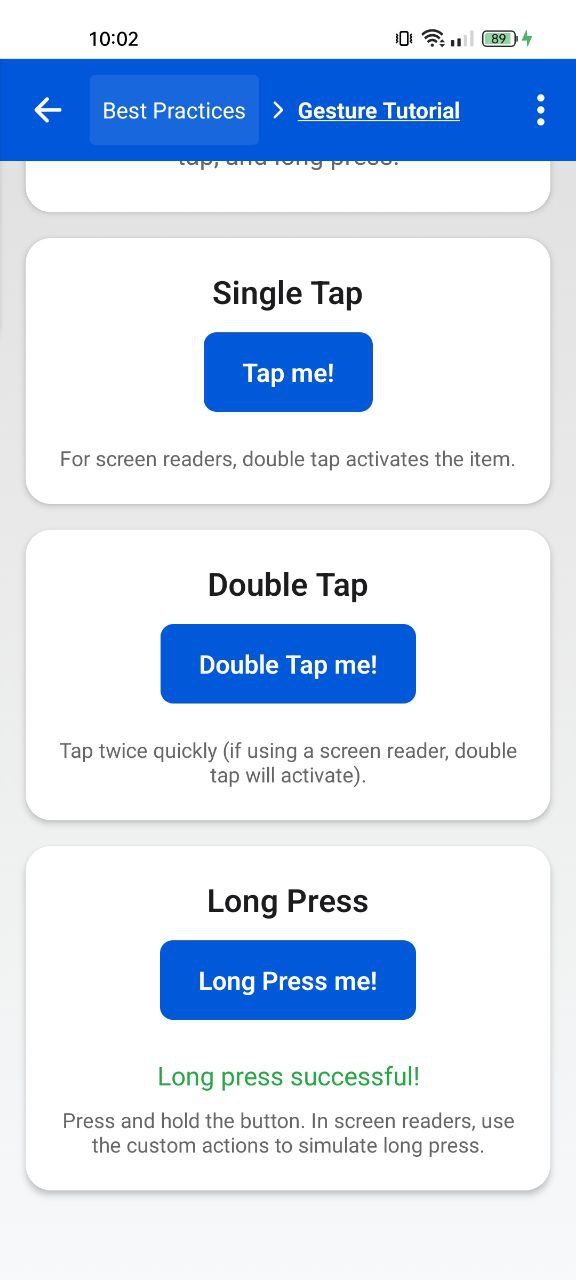
\includegraphics[width=\linewidth, alt={Second part of the Gestures tutorial screen}]{img/gestures2.jpg}
                \caption{Gestures tutorial screen - Part 2}
                \label{fig:gestures-right}
            \end{subfigure}
            \caption{Side-by-side view of the Gestures Tutorial screen sections}
            \label{fig:gestures_screens_sidebyside}
        \end{figure}

        \FloatBarrier

        \item \textit{Semantics Structure}: Here, developers learn about the importance of using semantic \textit{HTML} and \gls{ariag} roles to convey the structure and meaning of the application's content (\ref{fig:semantics_screens_sidebyside}). This helps screen readers and other assistive technologies better understand and navigate the application;

        \begin{figure}[ht]
            \centering
            \begin{subfigure}[b]{0.48\textwidth}
                \centering
                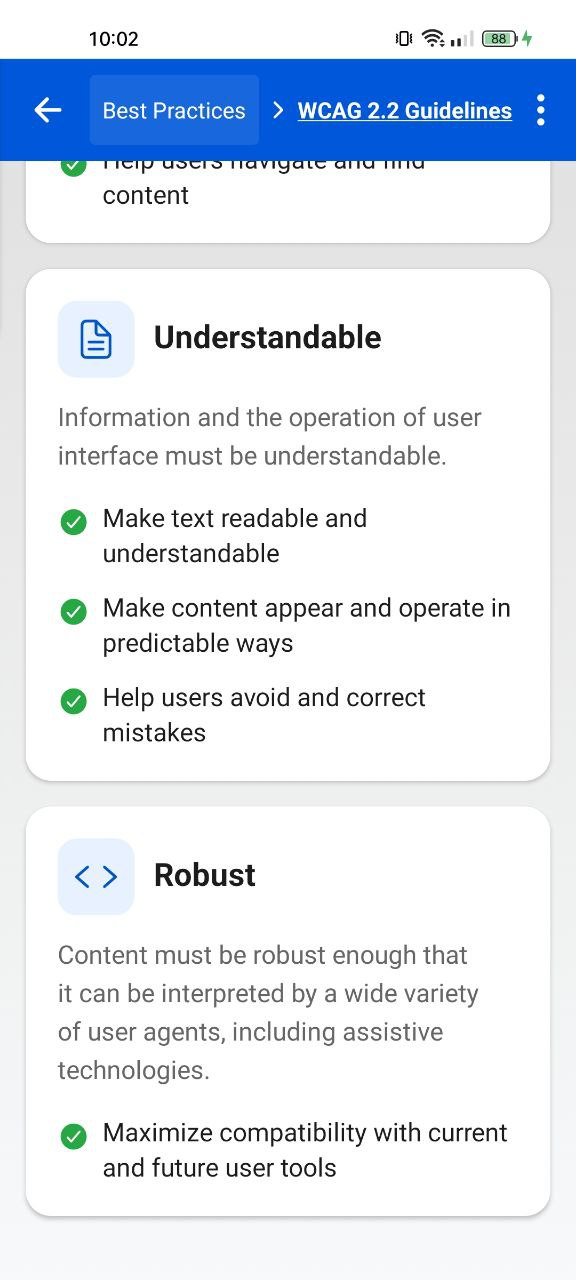
\includegraphics[width=\linewidth, alt={First part of the Semantic structure screen}]{img/semantics1.jpg}
                \caption{Semantic structure screen - Part 1}
                \label{fig:semantics-left}
            \end{subfigure}
            \hfill
            \begin{subfigure}[b]{0.48\textwidth}
                \centering
                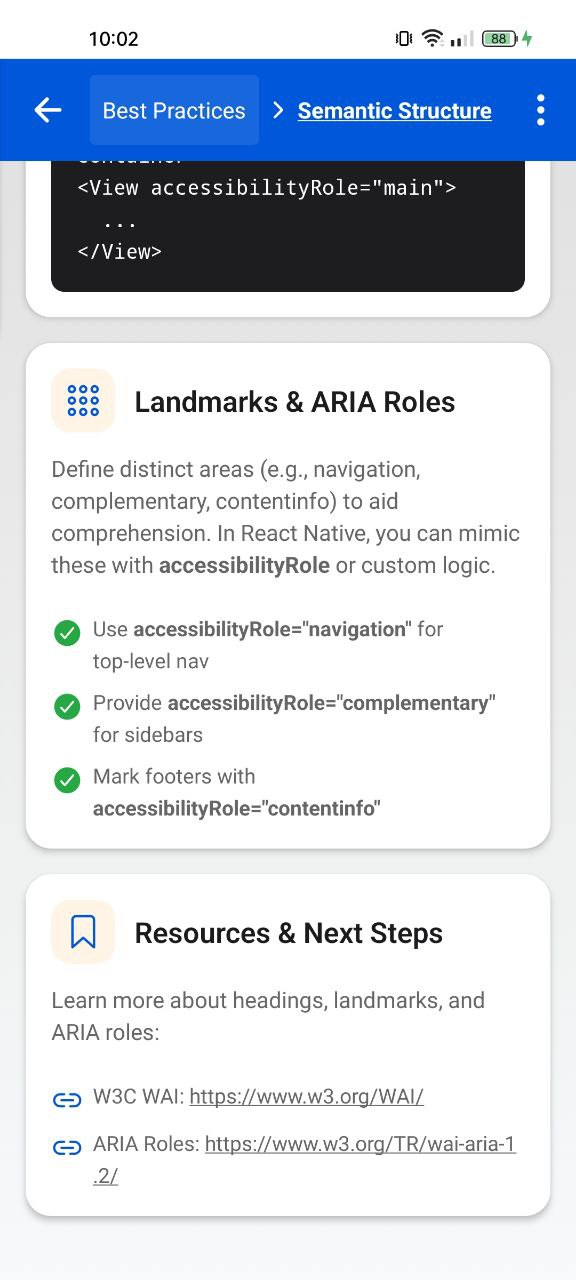
\includegraphics[width=\linewidth, alt={Second part of the Semantic structure screen}]{img/semantics2.jpg}
                \caption{Semantic structure screen - Part 2}
                \label{fig:semantics-right}
            \end{subfigure}
            \caption{Side-by-side view of the Semantic Structure screen sections}
            \label{fig:semantics_screens_sidebyside}
        \end{figure}

        \FloatBarrier

        \item \textit{Navigation}: This one focuses on creating accessible navigation patterns, such as menus, tabs, and breadcrumbs (\ref{fig:logical_screens_sidebyside}). It provides guidance on how to ensure that navigation elements are properly labeled, can be operated using various input methods, and provide clear feedback to the user, jumping directly to the main context of a screen and bringing the attention to an element on-screen without distracting him from the action to be completed;

        \begin{figure}[ht]
            \centering
            \begin{subfigure}[b]{0.48\textwidth}
                \centering
                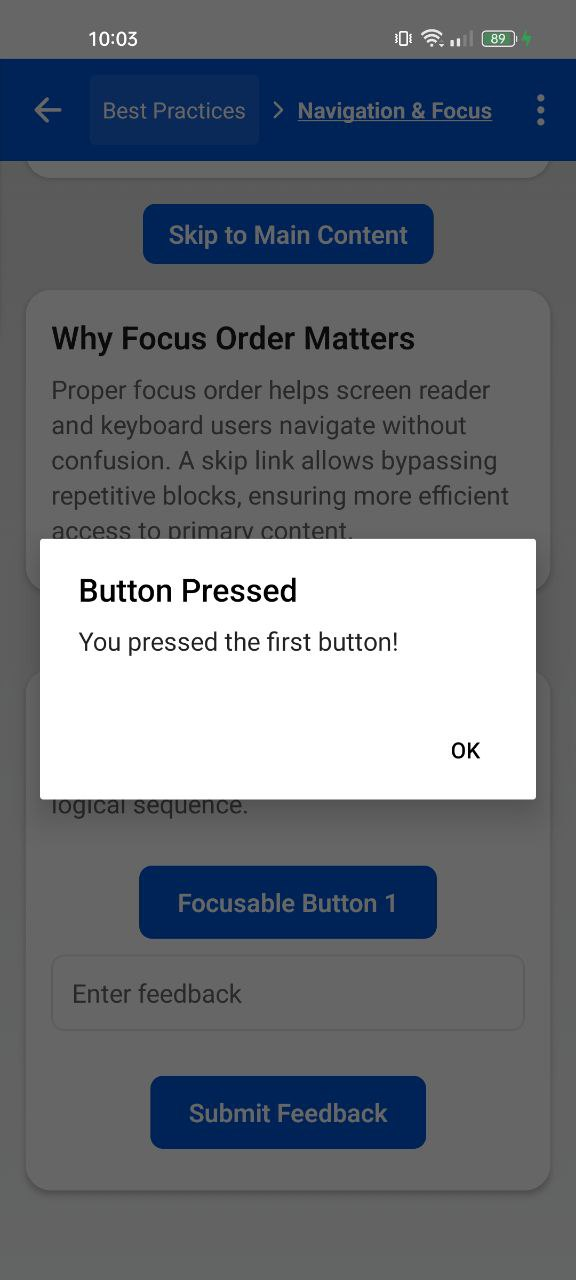
\includegraphics[width=\linewidth, alt={First part of the Logical navigation screen}]{img/logical1.jpg}
                \caption{Logical navigation screen - Part 1}
                \label{fig:logical-left}
            \end{subfigure}
            \hfill
            \begin{subfigure}[b]{0.48\textwidth}
                \centering
                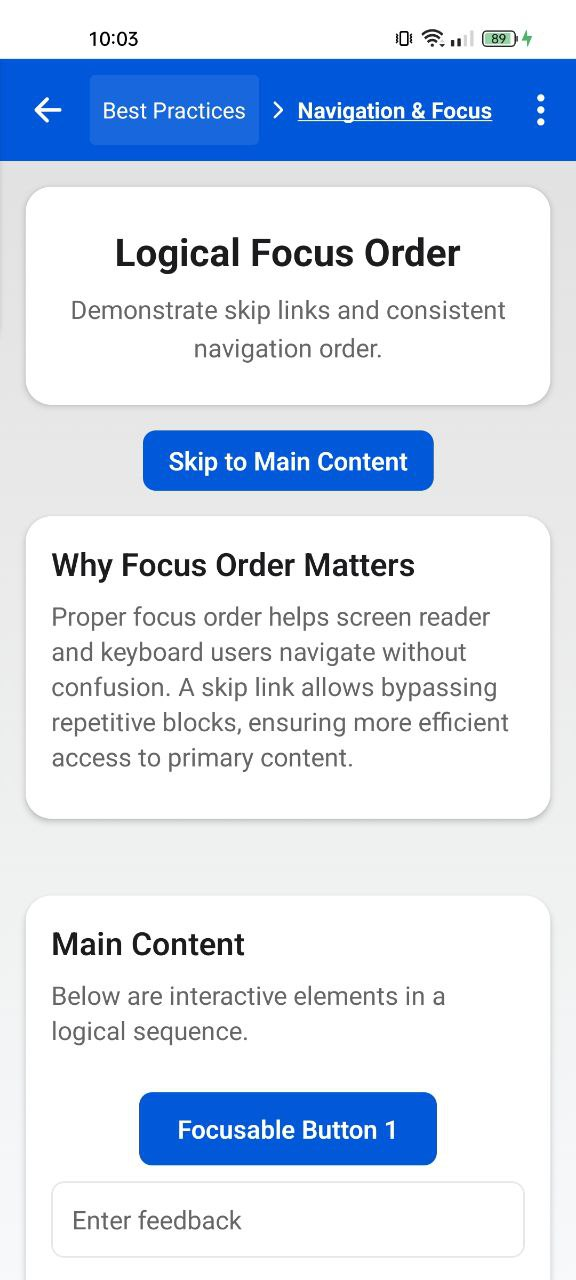
\includegraphics[width=\linewidth, alt={Second part of the Logical navigation screen}]{img/logical2.jpg}
                \caption{Logical navigation screen - Part 2}
                \label{fig:logical-right}
            \end{subfigure}
            \caption{Side-by-side view of the Logical navigation screen sections}
            \label{fig:logical_screens_sidebyside}
        \end{figure}

        \FloatBarrier

        \item \textit{Screen Reader Support}: This subscreen covers the specific considerations for making mobile applications compatible with screen readers, such as \gls{voiceover} on \textit{iOS} and \gls{talkback} on \textit{Android} (\ref{fig:screen_reader_screens_sidebyside}). It includes best practices for labeling elements, providing alternative text, and ensuring that the application's content and functionality can be fully accessed and understood using a screen reader;

        \begin{figure}[ht]
            \centering
            \begin{subfigure}[b]{0.48\textwidth}
                \centering
                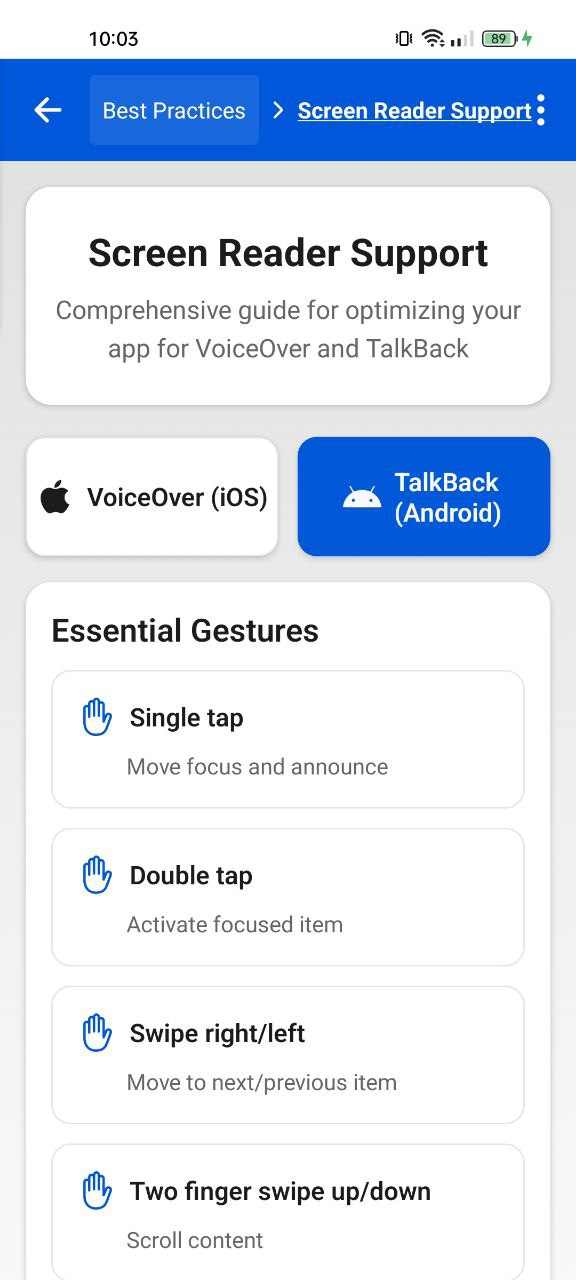
\includegraphics[width=\linewidth, alt={First part of the Screen reader support screen}]{img/screenreader1.jpg}
                \caption{Screen reader support screen - Part 1}
                \label{fig:screen-reader-left}
            \end{subfigure}
            \hfill
            \begin{subfigure}[b]{0.48\textwidth}
                \centering
                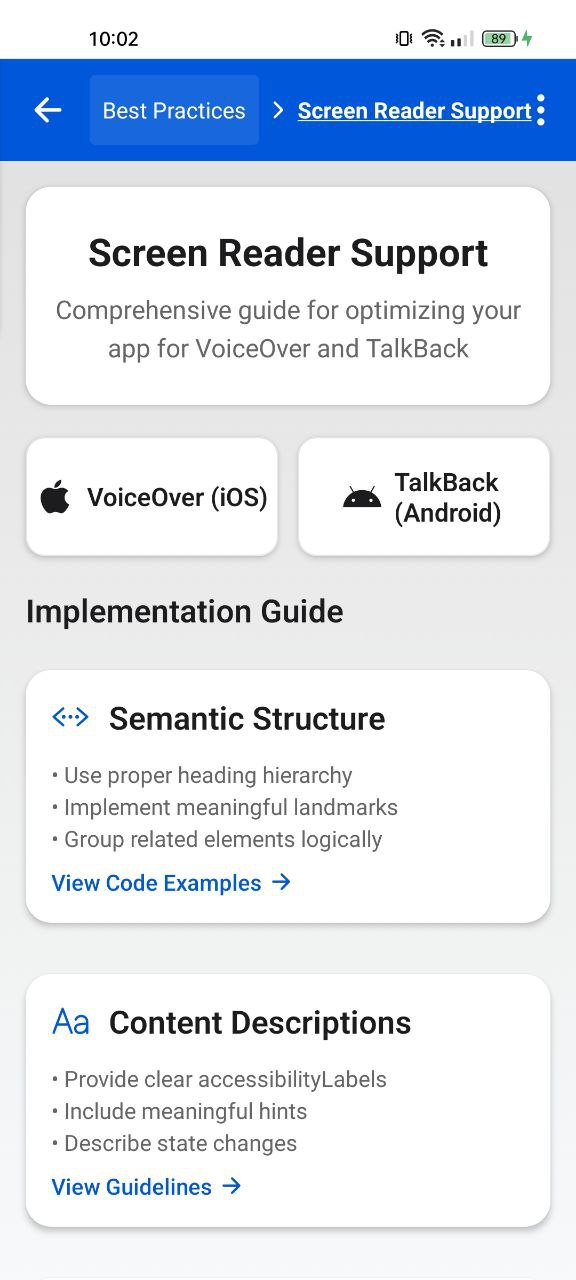
\includegraphics[width=\linewidth, alt={Second part of the Screen reader support screen}]{img/screenreader2.jpg}
                \caption{Screen reader support screen - Part 2}
                \label{fig:screen-reader-right}
            \end{subfigure}
            \caption{Side-by-side view of the Screen reader support screen sections}
            \label{fig:screen_reader_screens_sidebyside}
        \end{figure}

        \FloatBarrier

        \item \textit{Accessibility Guidelines}: The Accessibility Guidelines subscreen provides an overview of the key accessibility standards to be followed and a general list of principles to incorporate into a project, seeing how they apply to mobile application development (\ref{fig:guidelines_screens_sidebyside}). It helps developers understand the different levels of conformance and how to assess their application's accessibility against these guidelines.

        \begin{figure}[ht]
            \centering
            \begin{subfigure}[b]{0.48\textwidth}
                \centering
                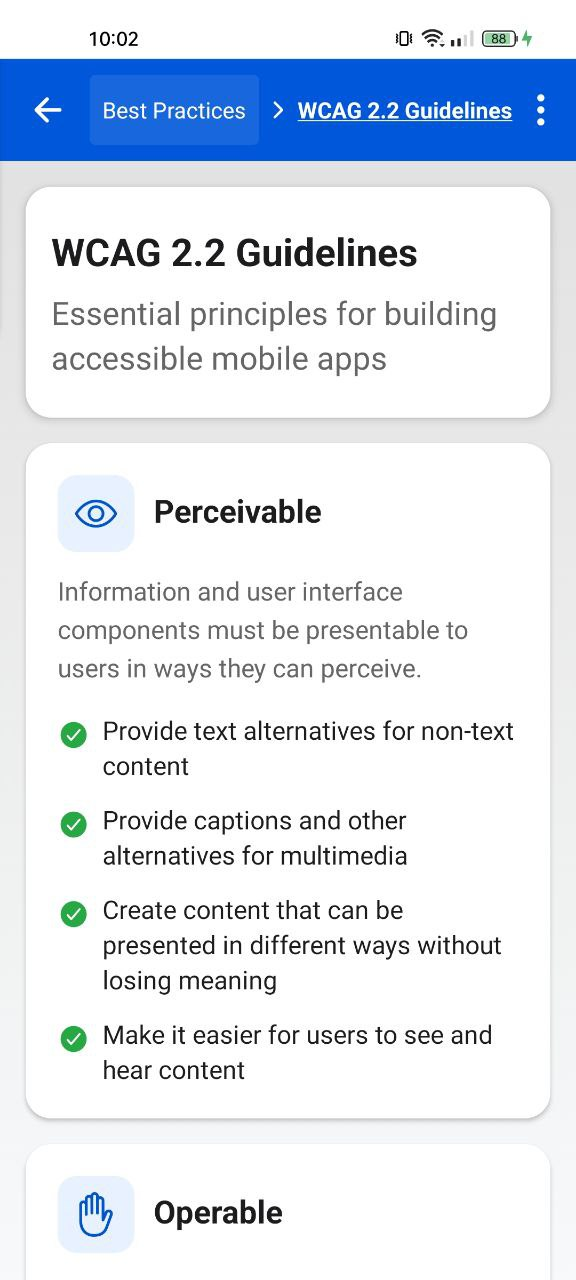
\includegraphics[width=\linewidth, alt={First part of the WCAG guidelines screen}]{img/guidelines1.jpg}
                \caption{Guidelines screen - Part 1}
                \label{fig:guidelines-left}
            \end{subfigure}
            \hfill
            \begin{subfigure}[b]{0.48\textwidth}
                \centering
                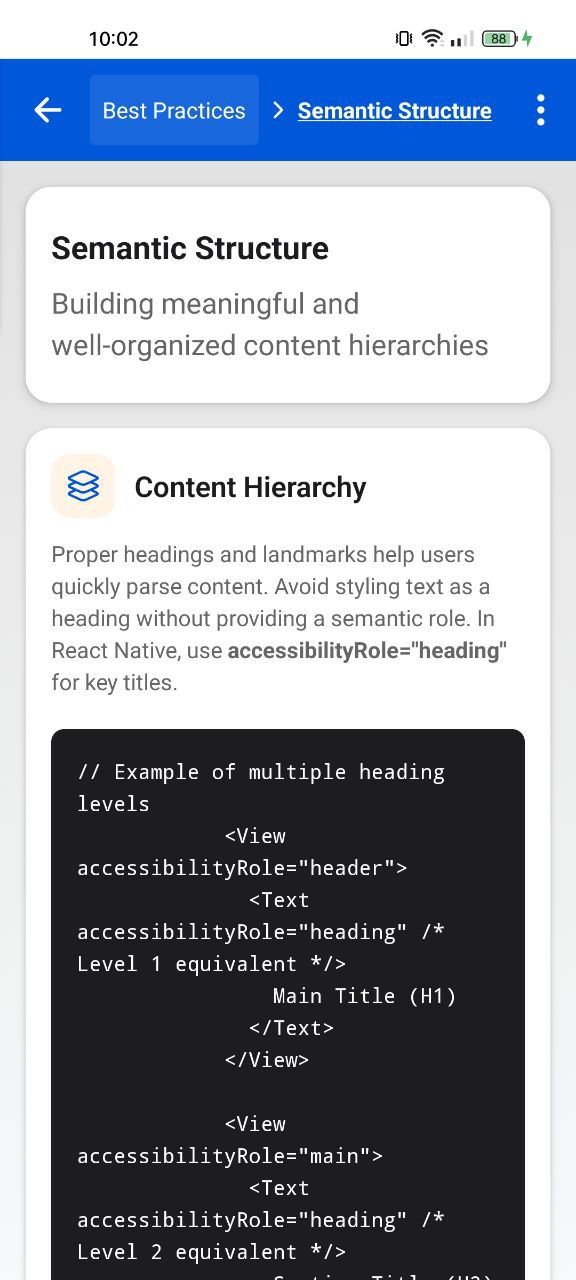
\includegraphics[width=\linewidth, alt={Second part of the WCAG guidelines screen}]{img/guidelines2.jpg}
                \caption{Guidelines screen - Part 2}
                \label{fig:guidelines-right}
            \end{subfigure}
            \caption{Side-by-side view of the WCAG Guidelines screen sections}
            \label{fig:guidelines_screens_sidebyside}
        \end{figure}

        \FloatBarrier
        
    \end{itemize}

\item \textbf{Framework Comparison} - It provides a side-by-side comparison of the accessibility features and implementation differences between popular mobile development frameworks, such as React Native and Flutter (\ref{fig:frameworks-comparison}). This section helps developers understand how accessibility is handled in each framework and provides guidance on leveraging the specific accessibility APIs and tools available in each one. This is divided into different categories, offering a practical and formal overview on how such frameworks are compared with each other. By structuring comparisons using consistent metrics, it teaches developers to evaluate accessibility implementation strategies based on objective criteria, reinforcing the quantitative approach introduced in the Home screen;

\begin{figure}[ht]
\centering
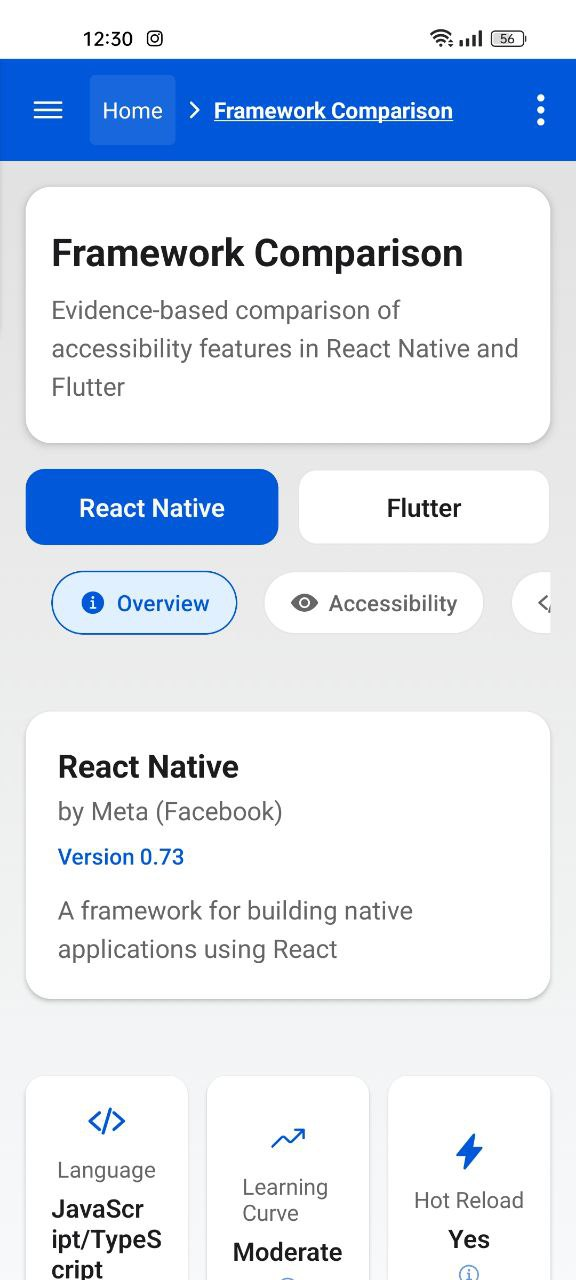
\includegraphics[width=0.4\linewidth, alt={Screenshot of the Framework comparison screen of AccessibleHub}]{img/frameworks-comparison.jpg}
\caption{The Framework comparison screen of \textit{AccessibleHub}}\label{fig:frameworks-comparison}
\end{figure}

\pagebreak

\item \textbf{Tools} - It serves as a central hub for accessing various accessibility-related tools and resources (\ref{fig:tools}). Each tool includes practical usage guidance, demonstrating workflow integration rather than isolated technical knowledge. This includes links to official documentation, such as the React Native Accessibility \acrshort{api} reference and the \textit{Flutter Accessibility package} documentation. It also provides quick access to popular accessibility testing tools, such as \textit{Accessibility Scanner} for \textit{Android} and \textit{Accessibility Inspector} for \textit{iOS}. This screen teaches developers that accessibility implementation is a continuous process spanning the entire development lifecycle; 

\begin{figure}[ht]
\centering
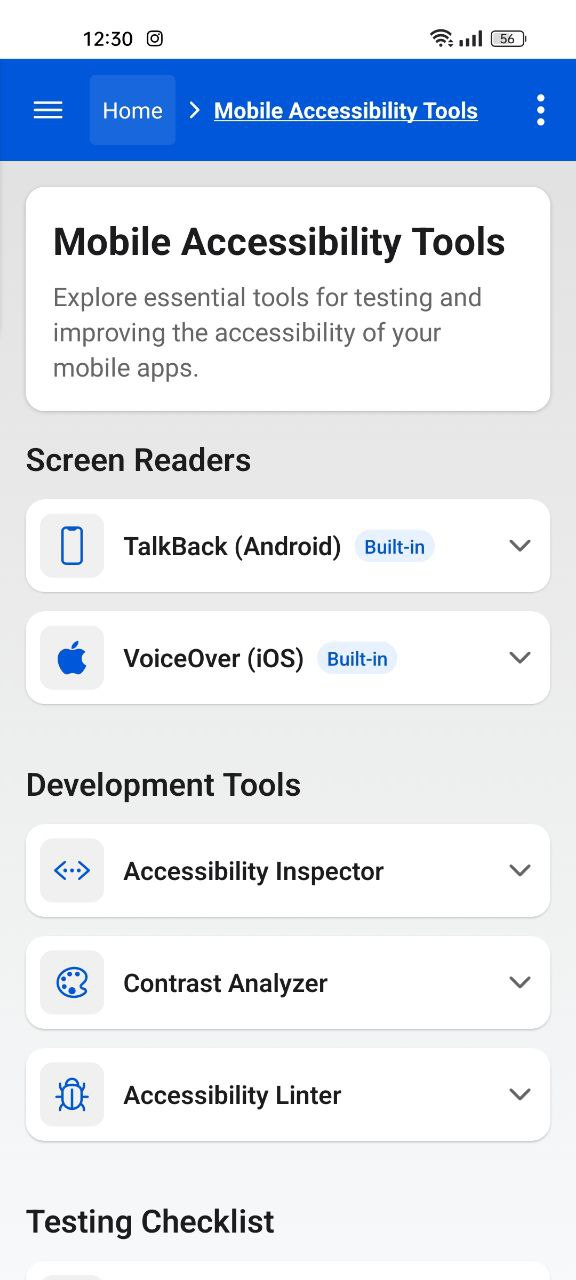
\includegraphics[width=0.4\linewidth, alt={Screenshot of the Tools screen of AccessibleHub}]{img/tools.jpg}
\caption{The Tools screen of \textit{AccessibleHub}}\label{fig:tools}
\end{figure}

\pagebreak

\item \textbf{Settings} - Allows users to customize various aspects of the \textit{AccessibleHub} application to suit their individual learning needs and preferences (\ref{fig:settings}). This includes options for adjusting the font size, color contrast (including options for gray scale and dark mode), reduced motion settings and others to help users and ensure the application itself is accessible to a wide range of users. By providing live demos of various accessibility adaptations (dark mode, contrast adjustment, text resizing), it allows developers to experience accessibility features firsthand, reinforcing the principle that accessibility is about personalization rather than one-size-fits-all solutions.

\begin{figure}[ht]
\centering
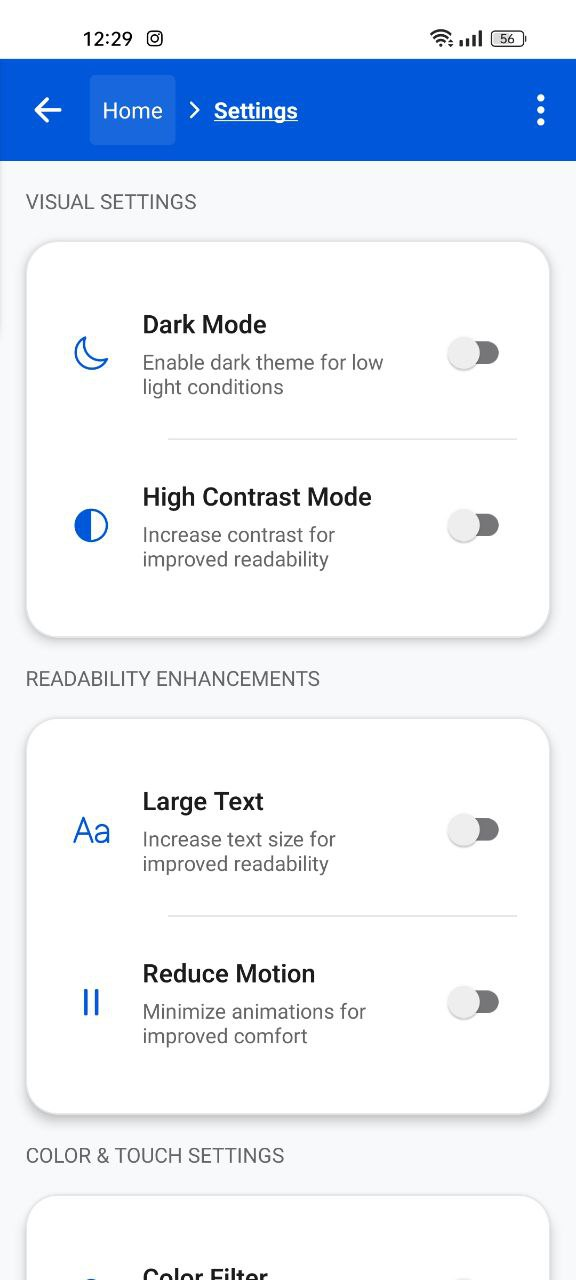
\includegraphics[width=0.4\linewidth, alt={Screenshot of the Settings screen of AccessibleHub}]{img/settings.jpg}
\caption{The Settings screen of \textit{AccessibleHub}}\label{fig:settings}
\end{figure}

\pagebreak

A key aspect of the Settings screen is its implementation of direct accessibility customization options. Figure~\ref{fig:settings_modes} illustrates the application in different accessibility modes.

\begin{figure}[ht]
    \centering
    \begin{subfigure}[b]{0.48\textwidth}
        \centering
        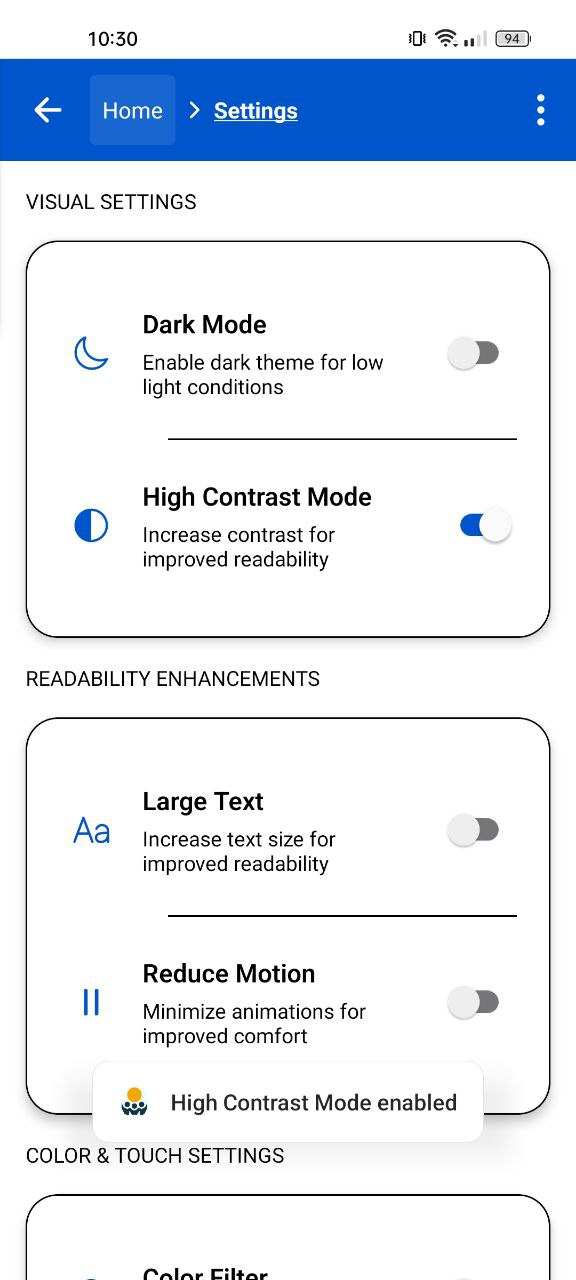
\includegraphics[width=\linewidth, alt={Settings screen with dark mode enabled}]{img/settings1.jpg}
        \caption{Dark mode enabled}
        \label{fig:settings-dark}
    \end{subfigure}
    \hfill
    \begin{subfigure}[b]{0.48\textwidth}
        \centering
        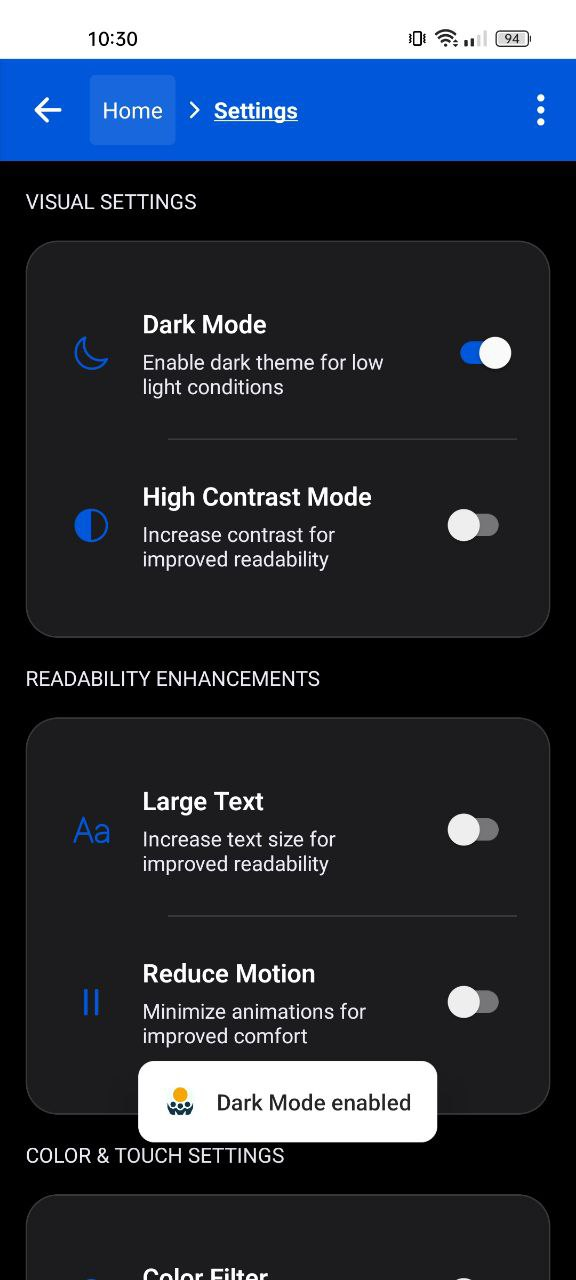
\includegraphics[width=\linewidth, alt={Settings screen with high contrast mode enabled}]{img/settings4.jpg}
        \caption{High contrast mode enabled}
        \label{fig:settings-contrast}
    \end{subfigure}
    \caption{Settings screen with different accessibility modes enabled}
    \label{fig:settings_modes}
\end{figure}

\pagebreak

Figure~\ref{fig:settings_notifications} demonstrates the visual feedback mechanisms when settings are toggled.

\begin{figure}[ht]
    \centering
    \begin{subfigure}[b]{0.48\textwidth}
        \centering
        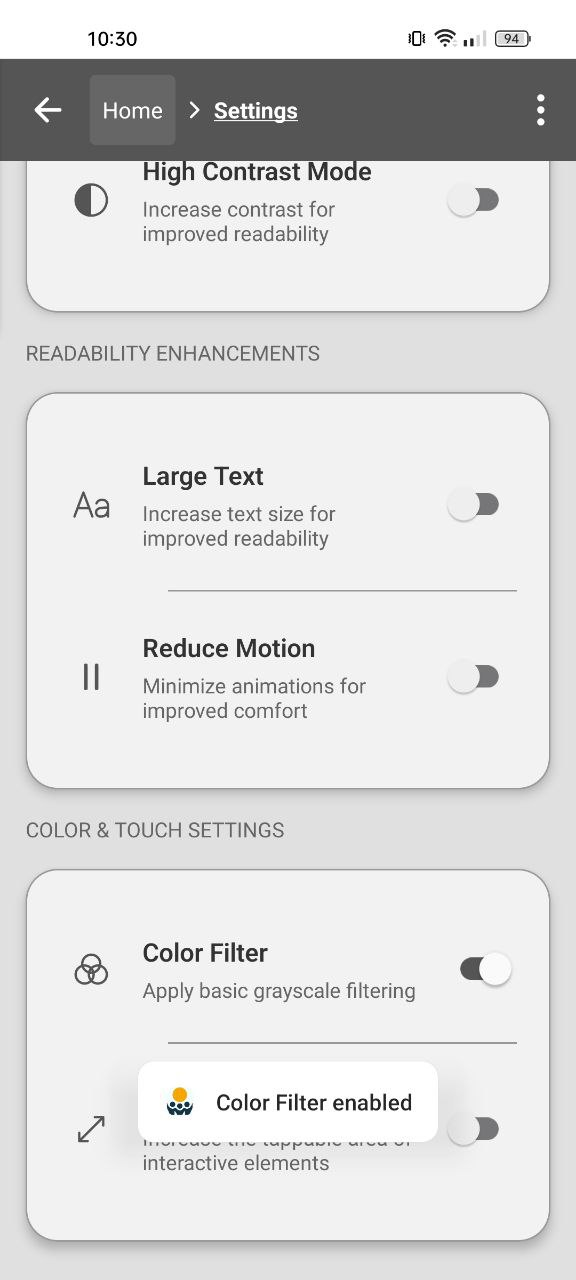
\includegraphics[width=\linewidth, alt={Settings screen with large text option enabled notification}]{img/settings3.jpg}
        \caption{Large text enabled notification}
        \label{fig:settings-text-notification}
    \end{subfigure}
    \hfill
    \begin{subfigure}[b]{0.48\textwidth}
        \centering
        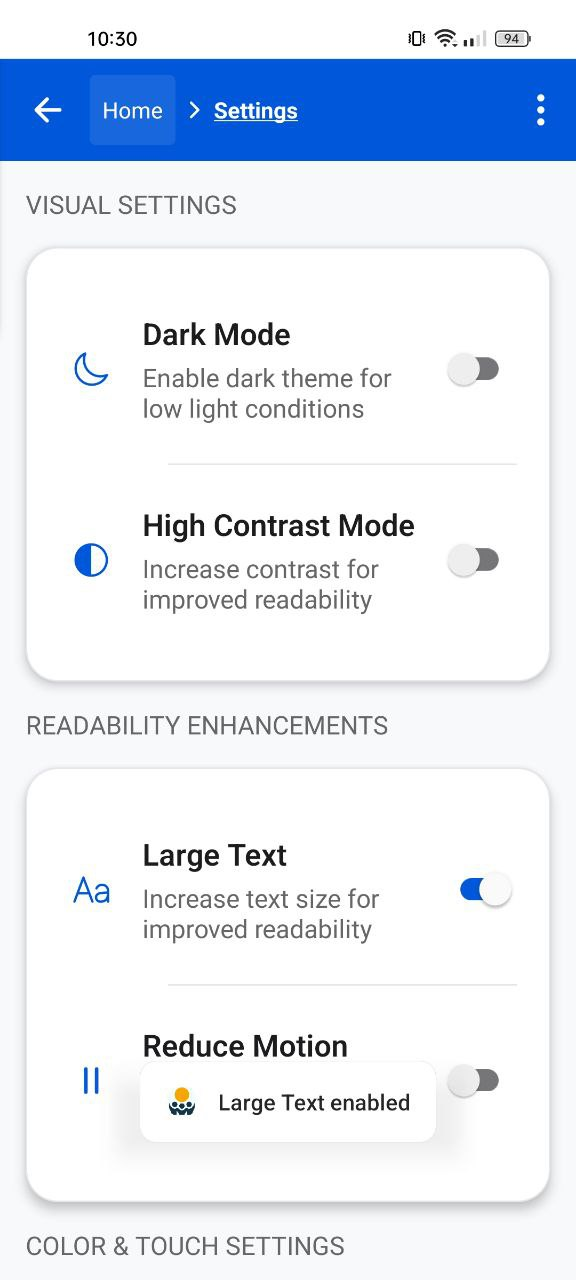
\includegraphics[width=\linewidth, alt={Settings screen with color filter enabled notification}]{img/settings2.jpg}
        \caption{Color filter enabled notification}
        \label{fig:settings-filter-notification}
    \end{subfigure}
    \caption{Visual notifications when accessibility settings are toggled}
    \label{fig:settings_notifications}
\end{figure}

\pagebreak

\item \textbf{Instruction and community} - It provides a collaborative learning environment that extends beyond technical implementation (\ref{fig:instruction-community}). This section offers developers an opportunity to dive deeper into accessibility knowledge through curated resources and community engagement allowing for easier exploration towards other online resources. This provides an overview of currently open projects in the field of accessibility, provides advices on specific plugins and offers community examples of interest for a developers to be motivated into the creation of other accessible projects. By providing a platform for continuous learning and collaboration, this screen reinforces the importance of accessibility as a collective effort and a fundamental aspect of modern mobile application development.

\begin{figure}[ht]
\centering
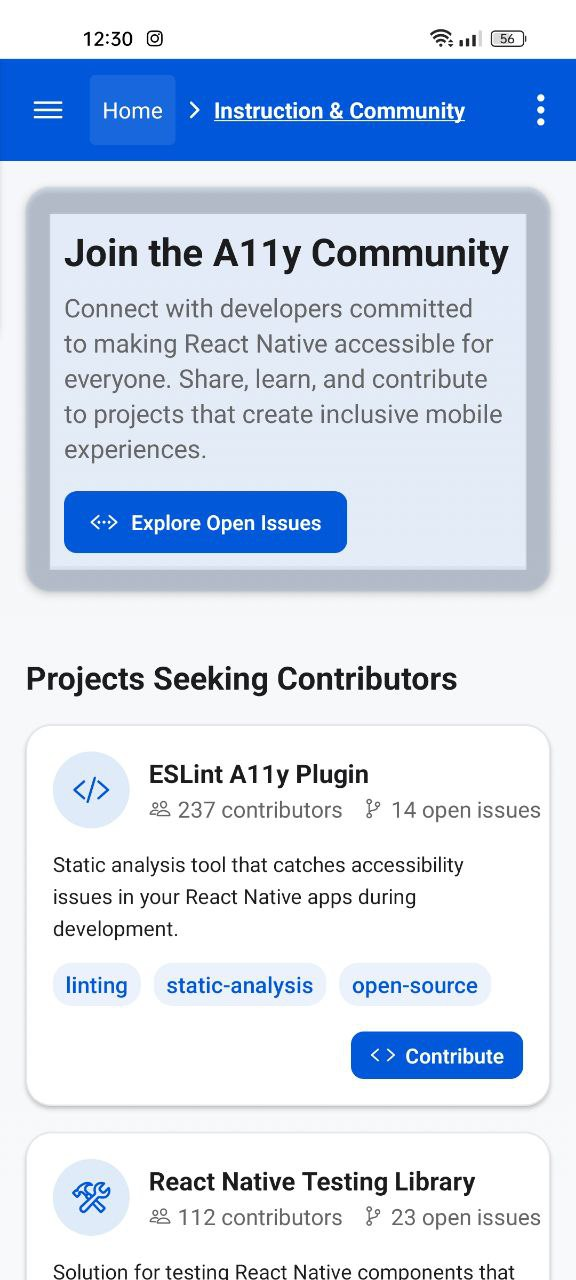
\includegraphics[width=0.4\linewidth, alt={Screenshot of the Instruction and community screen of AccessibleHub}]{img/instruction-community.jpg}
\caption{The Instruction and community screen of \textit{AccessibleHub}}\label{fig:instruction-community}
\end{figure}

\FloatBarrier
    
\end{enumerate}

\subsection{From guidelines to implementation: a screen-based methodology}
\label{sec:accessiblehub-screen-methodology}

Accessibility guidelines and standards - most notably the \acrshort{wcagacr}  and related mobile-specific considerations—establish the formal foundation for inclusive digital design, as discussed in \ref{sec:accessibility-guidelines}. These criteria are essential but inherently abstract and can be challenging to implement directly in code. Building on Perinello and Gaggi's approach focusing solely on post-implementation testing, the methodology presented embeds accessibility into the development process. We do this by analyzing each screen of the application through a structured framework that connects theoretical requirements with practical implementation strategies. The approach to be considered is built following these layers:

\begin{enumerate}
    \item \textit{Theoretical foundation} – This layer encompasses the abstract principles and success criteria defined by \textit{WCAG}/\acrshort{mcagacr}. For example, \textit{WCAG}’s four core principles require that content be presented in ways users can perceive, interact with, and understand. These criteria serve as the benchmark for our analysis;

    \item \textit{Implementation pattern} – Here, we translate the abstract requirements into concrete code structures within a mobile development context. In \textit{AccessibleHub}, this involves the systematic use of React Native properties (such as \textit{accessibilityLabel}, \textit{accessibilityRole}, etc.) to ensure that \acrshort{ui} components satisfy the established guidelines;

    \item \textit{User interaction flow} – Finally, we consider how end users interact with these components. This includes the behavior of assistive technologies (like screen readers), proper focus management, and the overall usability of the component within its real-world context.
\end{enumerate}

To illustrate this methodology in practice, we first map the \textit{UI} elements of a representative screen to their corresponding semantic roles. Next, we link each component to the relevant \acrshort{wcagacr} and \acrshort{mcagacr} criteria presented in the previous subsections, noting both the minimum compliance requirements and potential enhancements. Finally, we describe the technical solution—specifically, how React Native accessibility code properties are applied to meet and exceed these standards. This structured approach not only bridges the gap between abstract guidelines and real-world coding tasks but also sets the stage for the more detailed, screen-by-screen analyses presented in the next section. \\

To ensure alignment with the latest mobile accessibility standards, the \textit{AccessibleHub} analysis incorporates principles from the W3C's "Guidance on applying WCAG 2.2 to mobile applications" (WCAG2Mobile) \cite{w3c-wcag2mobile}. This authoritative interpretation adapts web-oriented accessibility criteria for mobile contexts, addressing unique challenges such as touch interactions, limited screen real estate, and platform-specific considerations. Throughout our screen-based methodology, we reference WCAG2Mobile's mobile-specific terminology and success criteria interpretations, particularly for component categories like touchable elements, forms, and media content. This integration ensures that \textit{AccessibleHub} provides guidance that is both theoretically sound and practically applicable in modern mobile development. 

\section{Accessibility implementation guidelines}
\label{sec:implementation-guidelines}

Having established the overall architecture of \textit{AccessibleHub} and the guiding principles from both \textit{WCAG} and \textit{MCAG}, we now present a screen-by-screen analysis. Each subsection highlights the key \textit{success criteria} addressed, references relevant \textit{mobile-specific considerations}, and demonstrates practical solutions in React Native. Where applicable, we contrast these with Flutter's approach, building upon the insights from Gaggi and Perinello's approach \cite{budai2024mobile} analyzying Budai's Flutter code - following guidelines and then giving advice into introducing new ones. These screens follow the structure presented in Section~\ref{sec:accessiblehub-educational-framework}, analyzed both as main screens and sections. \\ 

Below, a detailed analysis is given for the Home Screen and the Accessible Components main screen. For comprehensive, screen-by-screen analysis, readers are directed to the extended technical appendix available at \href{https://github.com/gabrielrovesti/AccessibleHub/blob/main/Technical\%20Thesis\%20Appendix/AccessibleHub\%20-\%20Extended\%20screen\%20analysis.pdf}{AccessibleHub Extended Screen Analysis} into §Chapter 1, where additional WCAG guidelines are introduced to accommodate future research on the field into §Chapter 2. Detailed mapping of the quoted WCAG2Mobile criteria to specific component implementations is also provided in the technical appendix.

\subsection{Home screen}

The Home screen serves as the primary entry point of the \textit{AccessibleHub} application. It provides key metrics on accessibility compliance (e.g., number of accessible components, WCAG conformance level) and navigation to sections: \textit{Accessible Components} (Quick Start), \textit{Best Practices}, \textit{Testing Tools}, and the \textit{Framework Comparison}. A screenshot of the interface is shown in Figure~\ref{fig:home_screens_sidebyside}.

\begin{figure}[ht]
    \centering
    \begin{subfigure}[b]{0.44\textwidth}
        \centering
        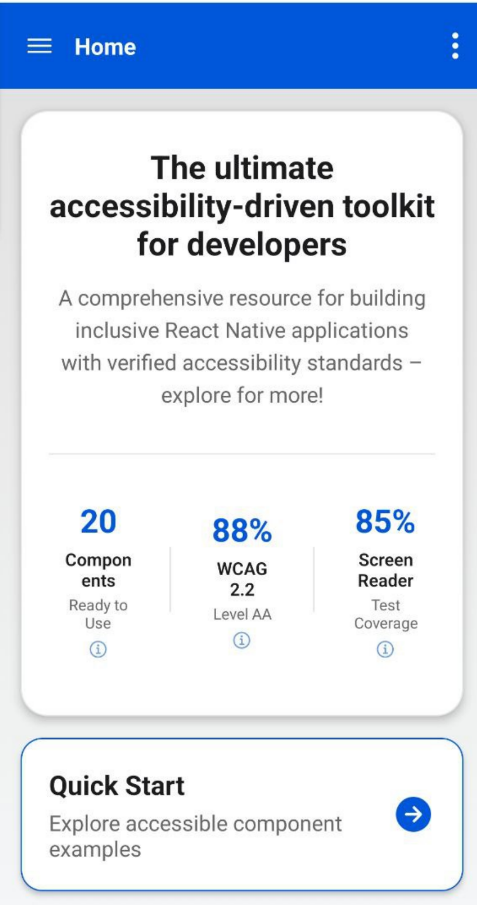
\includegraphics[width=\linewidth, alt={First part of the Home screen}]{img/home1.png}
        \caption{Home screen - Part 1}
        \label{fig:home-left}
    \end{subfigure}
    \hfill
    \begin{subfigure}[b]{0.48\textwidth}
        \centering
        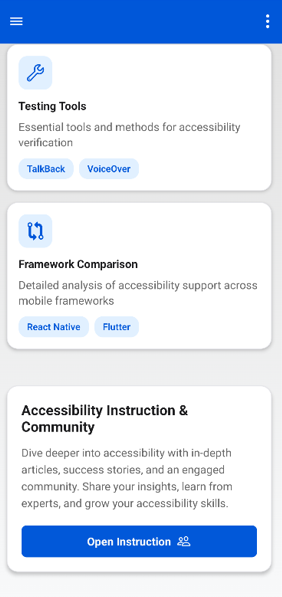
\includegraphics[width=\linewidth, alt={Second part of the Home screen}]{img/home2.png}
        \caption{Home screen - Part 2}
        \label{fig:home-right}
    \end{subfigure}
    \caption{Side-by-side view of the two Home sections, with metrics and navigation buttons}
    \label{fig:home_screens_sidebyside}
\end{figure}

\pagebreak

\subsubsection{Component inventory and WCAG/MCAG/WCAG2Mobile mapping}

Table~\ref{tab:component_criteria_mapping} provides a formal mapping between the UI components, their semantic roles, the specific WCAG 2.2 criteria they address, and their React Native implementation properties, with specific WCAG2Mobile considerations included.


\begin{longtable}[c]{|C{2.7cm}|C{1.8cm}|C{3cm}|C{3.5cm}|C{4.5cm}|}
\caption{Home screen component-criteria mapping with WCAG2Mobile considerations}
\label{tab:component_criteria_mapping}\\
\hline
\textbf{Component} & \textbf{Semantic Role} & \textbf{WCAG 2.2 Criteria} & \textbf{WCAG2Mobile Considerations} & \textbf{Implementation Properties} \\
\hline
\endfirsthead
\multicolumn{5}{c}%
{{\bfseries Table \thetable\ -- continued from previous page}} \\
\hline
\textbf{Component} & \textbf{Semantic Role} & \textbf{WCAG 2.2 Criteria} & \textbf{WCAG2Mobile Considerations} & \textbf{Implementation Properties} \\
\hline
\endhead
\hline
\multicolumn{5}{r}{{Continued on next page}} \\
\endfoot
\hline
\endlastfoot
Hero Title & header & 1.4.3 Contrast (AA)\newline 2.4.6 Headings (AA) & Text readability on variable screen sizes; Proper semantic structure in screen context & \texttt{accessibility \ Role="header"} \\
\hline
Stats Cards & button & 1.4.3 Contrast (AA)\newline 2.5.8 Target Size (AA)\newline 4.1.2 Name, Role, Value (A)\newline 2.4.9 Link Purpose (AAA) & Touch target optimization; Screen reader focus; Target tap area minimum of 44×44dp; Context-specific labeling & \texttt{accessibility \ Role="button"},\newline \texttt{accessibility \ Label="\$\{value\}\% \$\{type\}, tap for details"}\\
\hline
Decorative Icons & none & 1.1.1 Non-text Content (A) & Reduction of unnecessary focus stops; Efficiency in screen reader navigation sequence & \texttt{accessibility \ ElementsHidden=true},\newline \texttt{important \ ForAccessibility="no"} \\
\hline
Quick Start Button & button & 1.4.3 Contrast (AA)\newline 2.5.8 Target Size (AA)\newline 2.5.2 Pointer Cancellation (A)\newline 2.4.10 Section Headings (AAA) & One-handed operation; Clear touch feedback; Sufficient tap target area exceeding minimum requirements & \texttt{accessibility \ Role="button"},\newline \texttt{minHeight: 48},\newline \texttt{minWidth: 150} \\
\hline
Feature Cards & button & 1.3.1 Info and Relationships (A)\newline 1.4.3 Contrast (AA)\newline 2.5.8 Target Size (AA)\newline 3.2.5 Change on Request (AAA) & Logical grouping; Clear component boundaries; Screen reader context preservation & \texttt{accessibility \ Role="button"},\newline \texttt{accessibility \ Label="\$\{title\}"},\newline \texttt{accessibility \ Hint="\$\{hint\}"} \\
\hline
Modal Dialog & dialog & 2.4.3 Focus Order (A)\newline 4.1.2 Name, Role, Value (A)\newline 2.4.8 Location (AAA) & Focus management in modal context; Proper dialog role in mobile screen context; Keyboard trap prevention & \texttt{accessibility \ Role="dialog"},\newline Focus management implementation \\
\hline
Modal Tabs & tablist & 2.4.7 Focus Visible (AA)\newline 4.1.2 Name, Role, Value (A)\newline 2.4.9 Link Purpose (AAA) & Touch interaction patterns; State communication; Active tab indication for screen readers & \texttt{accessibility \ Role="tablist"},\newline \texttt{accessibility \ State=\{\{ selected: isActive \}\}} \\
\end{longtable}

\FloatBarrier

\subsubsection{Formal metrics calculation methodology}

The Home screen displays three key metrics that provide quantitative measurements of the application's accessibility. These metrics are calculated using a formal methodology defined in the \texttt{calculateAccessibilityScore} function within \texttt{index.tsx}, as shown by Figure~\ref{fig:wcag_modal_pair} and Figure~\ref{fig:component_modal_pair}.

\begin{figure}[ht]
    \centering
    \begin{subfigure}[b]{0.48\textwidth}
        \centering
        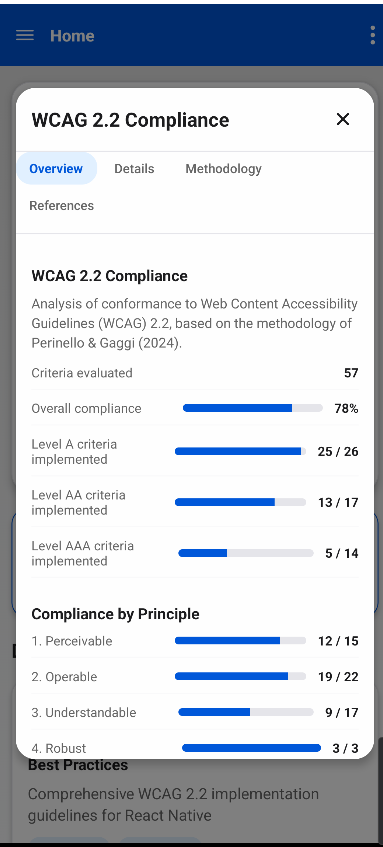
\includegraphics[width=\linewidth]{img/wcag-compliance.png}
        \caption{WCAG compliance overview}
        \label{fig:wcag-compliance-modal}
    \end{subfigure}
    \hfill
    \begin{subfigure}[b]{0.48\textwidth}
        \centering
        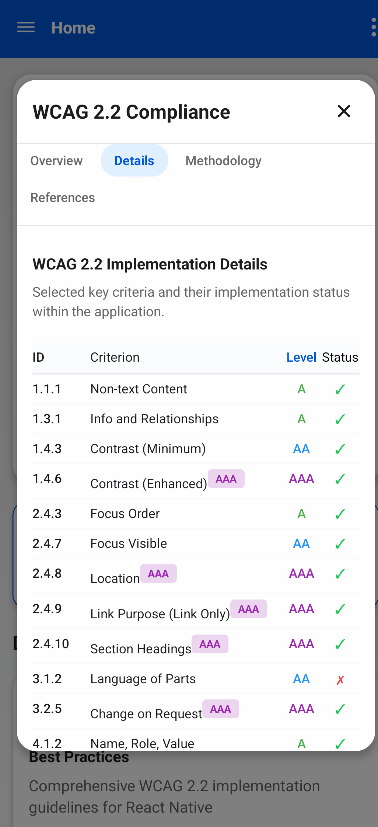
\includegraphics[width=\linewidth]{img/wcag-compliance-details.png}
        \caption{WCAG compliance details}
        \label{fig:wcag-details-modal}
    \end{subfigure}
    \caption{Modal dialogs showing WCAG compliance metrics}
    \label{fig:wcag_modal_pair}
\end{figure}

\begin{figure}[ht]
    \centering
    \begin{subfigure}[b]{0.48\textwidth}
        \centering
        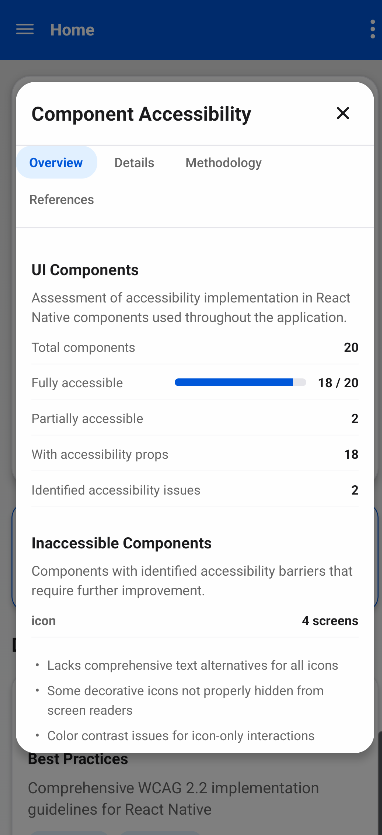
\includegraphics[width=\linewidth]{img/component-modal.png}
        \caption{Component metrics overview}
        \label{fig:component-overview-modal}
    \end{subfigure}
    \hfill
    \begin{subfigure}[b]{0.48\textwidth}
        \centering
        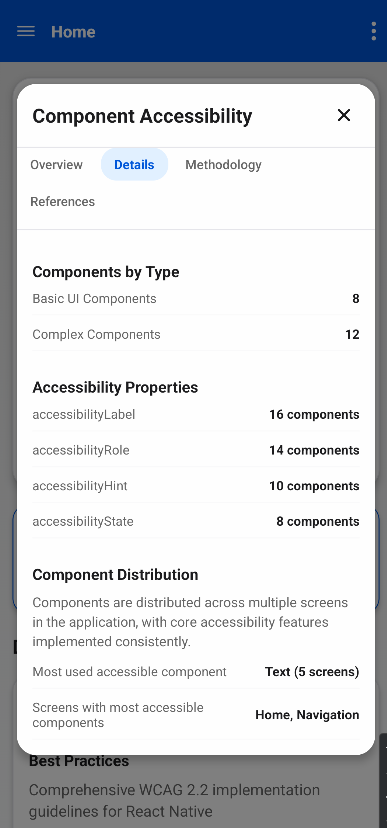
\includegraphics[width=\linewidth]{img/component-details.png}
        \caption{Component metrics details}
        \label{fig:component-details-modal}
    \end{subfigure}
    \caption{Modal dialogs showing component accessibility metrics}
    \label{fig:component_modal_pair}
\end{figure}

\FloatBarrier

An overview of the test done with screen reader with the methodology and references adopted is present in Figure~\ref{fig:screen_reader_modals} and Figure~\ref{fig:methodology_references}.

\begin{figure}[ht]
    \centering
    \begin{subfigure}[b]{0.48\textwidth}
        \centering
        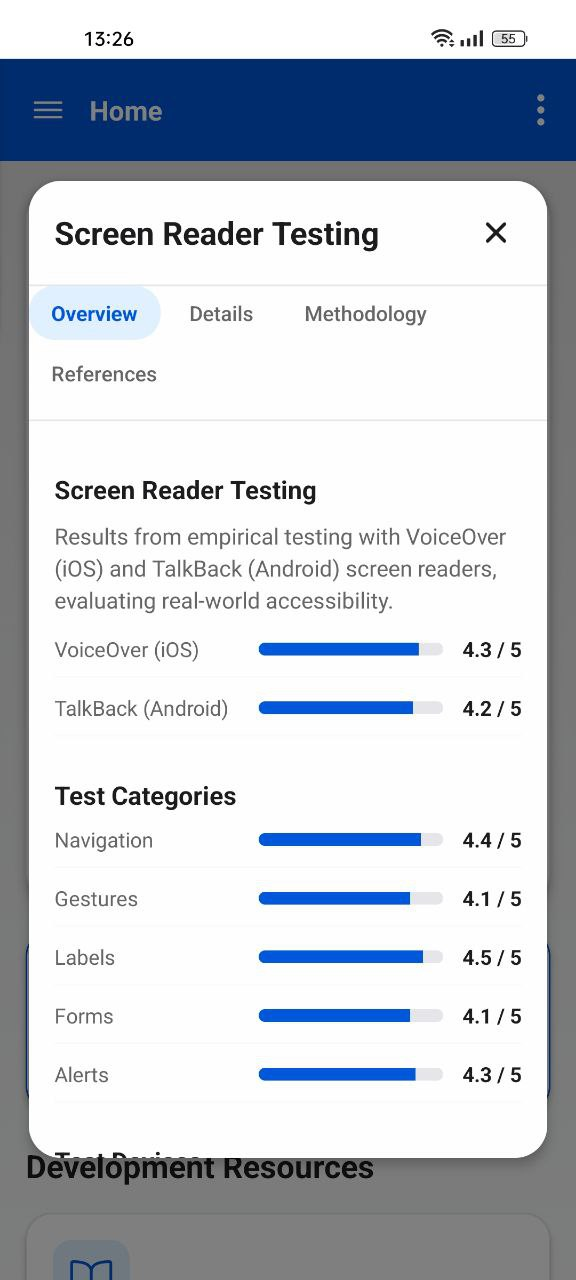
\includegraphics[width=\linewidth]{img/screen-reader-modal.jpg}
        \caption{Screen reader testing overview}
        \label{fig:screen-reader-overview}
    \end{subfigure}
    \hfill
    \begin{subfigure}[b]{0.48\textwidth}
        \centering
        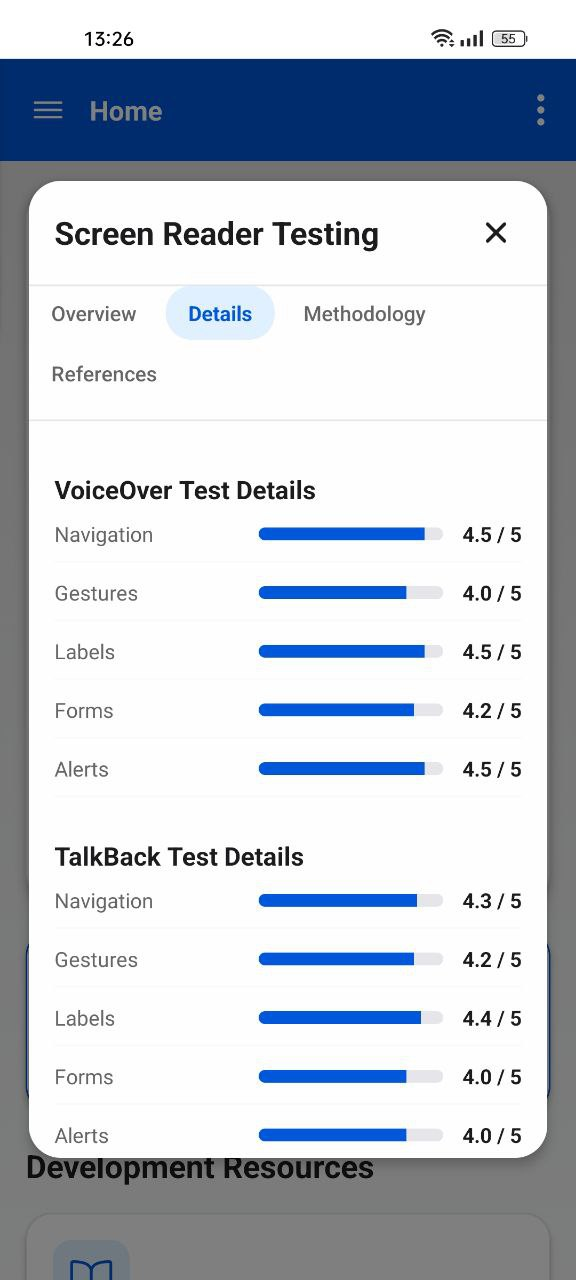
\includegraphics[width=\linewidth]{img/screen-reader-details.jpg}
        \caption{Screen reader testing details}
        \label{fig:screen-reader-details}
    \end{subfigure}
    \caption{Modal dialogs showing screen reader testing metrics}
    \label{fig:screen_reader_modals}
\end{figure}

\begin{figure}[ht]
    \centering
    \begin{subfigure}[b]{0.48\textwidth}
        \centering
        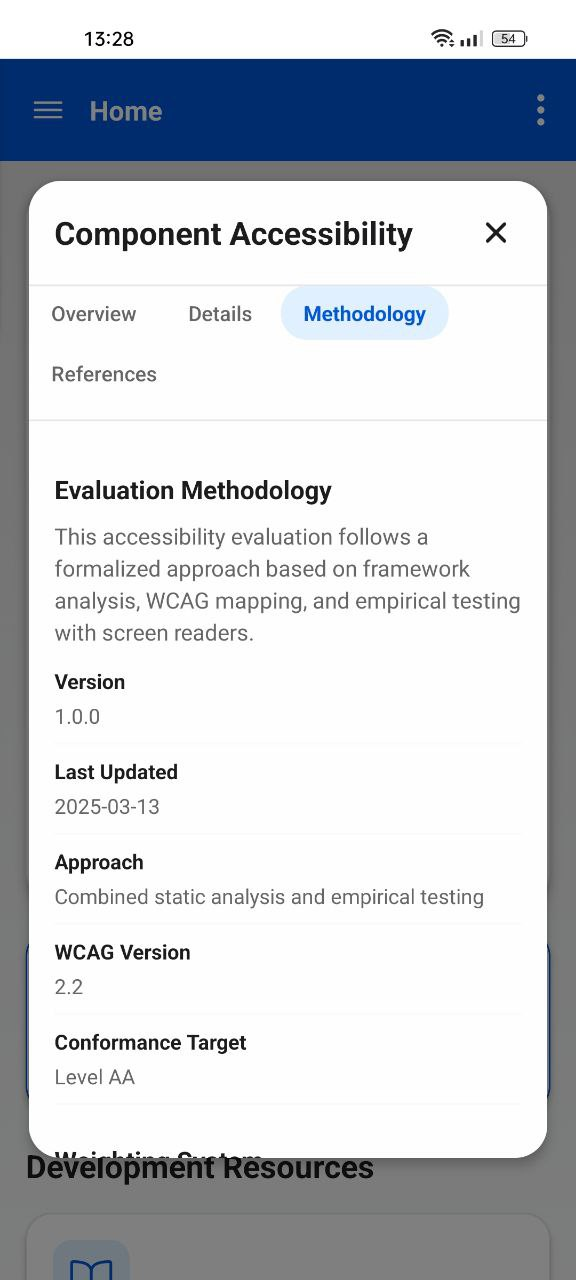
\includegraphics[width=\linewidth]{img/methodology.jpg}
        \caption{Methodology explanation}
        \label{fig:methodology-modal}
    \end{subfigure}
    \hfill
    \begin{subfigure}[b]{0.48\textwidth}
        \centering
        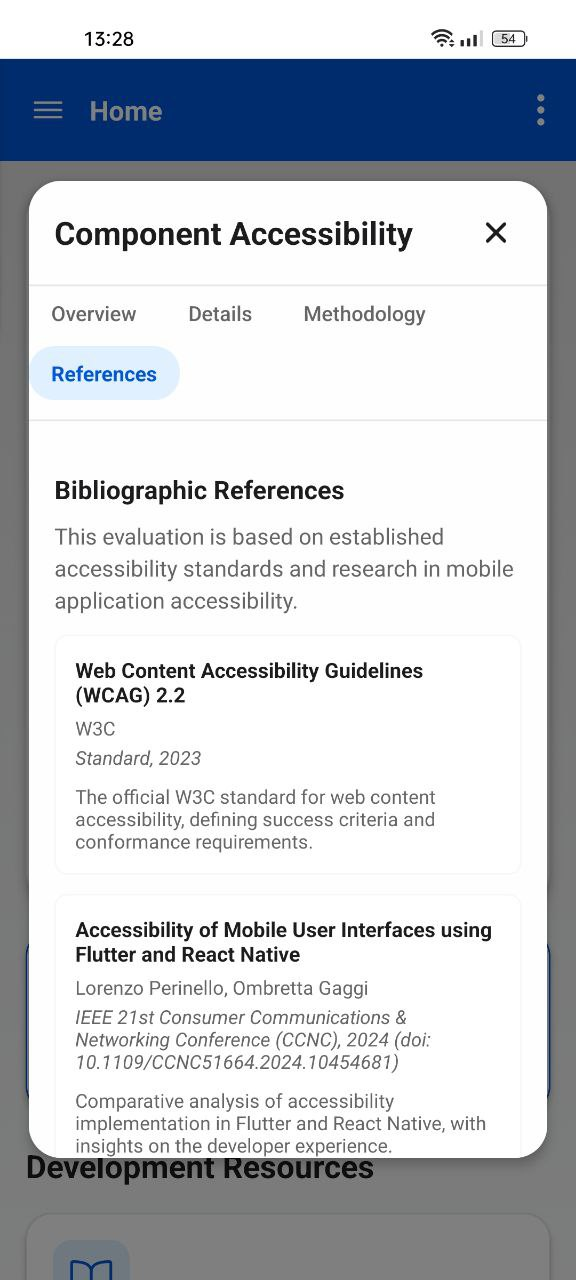
\includegraphics[width=\linewidth]{img/references.jpg}
        \caption{References documentation}
        \label{fig:references-modal}
    \end{subfigure}
    \caption{Modal dialogs showing methodology and references}
    \label{fig:methodology_references}
\end{figure}

\paragraph{Component Accessibility Score}

The Component Accessibility Score (CAS) is calculated using the following formula:
\begin{equation}
\text{ComponentScore}
= \left(\frac{\text{AccessibleComponents}}{\text{TotalComponents}}\right) \times 100
\end{equation}
Where:
\begin{itemize}
    \item \texttt{AccessibleComponents} = Number of components with properly implemented accessibility attributes (20);
    \item \texttt{TotalComponents} = Total number of UI components used in the application (20).
\end{itemize}

The application implements 20 distinct UI components divided into two primary categories:
\begin{itemize}

\item 8 basic UI components (\texttt{button}, \texttt{text}, \texttt{image}, \texttt{touchableOpacity}, \texttt{scrollView}, \texttt{view}, \texttt{textInput}, \texttt{switch}) that provide essential interaction capabilities;

\item 12 complex UI components (\texttt{card}, \texttt{icon}, \texttt{linearGradient}, \texttt{modal}, \texttt{alert}, \texttt{skipLink}, \texttt{listItem}, \texttt{tabNavigator}, \texttt{checklistItem}, \texttt{buttonGroup}, \texttt{slider}, \texttt{datePicker}) that offer more sophisticated user interaction patterns.

\end{itemize}
Each component is tracked across multiple screens to ensure consistent accessibility implementation throughout the application. For example, the \texttt{text} component appears in 5 different screens, while specialized components like \texttt{datePicker} are used in specific functional areas. This comprehensive tracking system enables precise measurement of accessibility implementation across the application's component ecosystem.

The implementation in \texttt{index.tsx} maintains a formal registry of all UI components, as shown in Listing~\ref{lst:component-registry}.

\begin{lstlisting}[
  style=ReactNativeStyle,
  caption={Component registry and calculation},
  label={lst:component-registry},
  basicstyle=\ttfamily\footnotesize,
  numbers=left,
]
// Component registry with accessibility status tracking
  const componentsRegistry = {
  // Basic UI components
  'button': { implemented: true, accessible: true,
   screens: ['home', 'gestures', 'navigation'] },
  'text': { implemented: true, accessible: true,
  screens: ['home', 'guidelines', 'navigation', 'screen-reader', 'semantics'] },
  
// ... other basic components

// Complex UI components
'card': { implemented: true, accessible: true,
screens: ['home', 'guidelines', 'navigation', 'screen-reader', 'semantics'] },
'icon': { implemented: true, accessible: true,
screens: ['home', 'guidelines', 'screen-reader', 'semantics'] },

// ... other complex components
};

// Component calculation
const componentsTotal = Object.keys(componentsRegistry).length;
const accessibleComponents = Object.values(componentsRegistry)
  .filter(c => c.implemented && c.accessible).length;
const componentScore = Math.round((accessibleComponents / 
  componentsTotal) * 100);
\end{lstlisting}

\FloatBarrier

\paragraph{WCAG compliance score}

The WCAG compliance score employs a weighted approach that prioritizes fundamental accessibility requirements while acknowledging the aspirational nature of higher-level criteria:
\begin{align}
\text{WCAGCompliance} = \Bigg(&\left(\frac{\text{AAndAAImplemented}}{\text{AAndAACriteria}}\right) \times 0.8 + \
&\left(\frac{\text{AllImplemented}}{\text{AllCriteria}}\right) \times 0.2\Bigg) \times 100
\end{align}
Where:
\begin{itemize}
\item \texttt{AAndAAImplemented} = Number of Level A and AA success criteria implemented;
\item \texttt{AAndAACriteria} = Total number of Level A and AA criteria;
\item \texttt{AllImplemented} = Number of all criteria implemented (including AAA);
\item \texttt{AllCriteria} = Total number of all criteria across all levels.
\end{itemize}
This weighted approach acknowledges that Level A and AA criteria represent essential accessibility requirements that must be implemented for basic conformance (80\% of the weight), while Level AAA criteria represent more advanced and specialized enhancements (20\% of the weight), implemented for the highest standard of accessibility. 

To enable more granular analysis, extended variables are introduced to preserve formal criteria and compliance levels reached:
\begin{itemize}
\item \texttt{CriteriaLevelAMet} = Number of Level A success criteria implemented (25);
\item \texttt{CriteriaLevelAAMet} = Number of Level AA success criteria implemented (13);
\item \texttt{CriteriaLevelAAAMet} = Number of Level AAA success criteria implemented (9);
\item \texttt{LevelACompliance}, \texttt{LevelAACompliance}, \texttt{LevelAAACompliance} = Percentage of criteria met at each level.
\end{itemize}

The implementation maintains a comprehensive tracking system for WCAG criteria, as shown in Listing~\ref{lst:wcag-tracking}.
\begin{lstlisting}[
style=ReactNativeStyle,
caption={WCAG criteria tracking and calculation},
label={lst:wcag-tracking},
basicstyle=\ttfamily\footnotesize,
numbers=left,
]
// WCAG criteria tracking with implementation status
const wcagCriteria = {
'1.1.1': { level: 'A', implemented: true,
name: "Non-text Content" },
'1.3.1': { level: 'A', implemented: true,
name: "Info and Relationships" },
// ... other A and AA criteria
'2.4.8': { level: 'AAA', implemented: true,
name: "Location" },
'2.4.9': { level: 'AAA', implemented: true,
name: "Link Purpose (Link Only)" },
'2.4.10': { level: 'AAA', implemented: true,
name: "Section Headings" },
'3.2.5': { level: 'AAA', implemented: true,
name: "Change on Request" },
// ... other criteria
};

// Simplified calculation for UI display
const criteriaValues = Object.values(wcagCriteria);
const aAndAACriteria = criteriaValues.filter(c => c.level === 'A' || c.level === 'AA');
const aAndAAImplemented = aAndAACriteria.filter(c => c.implemented).length;
const allImplemented = criteriaValues.filter(c => c.implemented).length;
const allCriteria = criteriaValues.length;

// 80% based on A & AA, 20% based on overall
const wcagCompliance = Math.round(
(((aAndAAImplemented / aAndAACriteria.length) * 0.8) +
((allImplemented / allCriteria) * 0.2)) * 100
);

// Detailed tracking (preserved but not displayed in UI)
const levelACriteria = criteriaValues.filter(c => c.level === 'A').length;
const levelACriteriaMet = criteriaValues
.filter(c => c.level === 'A' && c.implemented).length;
const levelACompliance = Math.round((levelACriteriaMet / levelACriteria) * 100);
// Same for other levels...

\end{lstlisting}

\FloatBarrier

\paragraph{Screen reader testing score}

The Screen Reader Testing Score represents empirical testing with VoiceOver (iOS) and TalkBack (Android):

\begin{equation}
\text{TestingScore} 
= \left(\frac{\text{VoiceOverAvg} + \text{TalkBackAvg}}{2}\right) \times 20
\end{equation}

Where:
\begin{itemize}
    \item \texttt{VoiceOverAvg} = Average score from VoiceOver testing across categories (4.34/5);
    \item \texttt{TalkBackAvg} = Average score from TalkBack testing across categories (4.18/5).
\end{itemize}

The methodology employs a Likert scale (where 5 represents perfect implementation) across five key categories that represent essential aspects of screen reader interaction:
\begin{itemize}
\item \textit{Navigation}: Logical flow and ease of traversing the interface (VoiceOver: 4.5, TalkBack: 4.3)
\item \textit{Gestures}: Recognition and consistency of touch gestures (VoiceOver: 4.0, TalkBack: 4.2)
\item \textit{Labels}: Clarity and completeness of element descriptions (VoiceOver: 4.5, TalkBack: 4.4)
\item \textit{Forms}: Accessibility of input controls and feedback (VoiceOver: 4.2, TalkBack: 4.0)
\item \textit{Alerts}: Proper announcement of dialogs and notifications (VoiceOver: 4.5, TalkBack: 4.0)
\end{itemize}

The scale range of 4.0-4.9 represents "good to excellent" implementation quality, with no score falling below 4.0, indicating that all tested areas meet professional accessibility standards. The multiplication by 20 normalizes the 1-5 scale to a percentage format (0-100\%) to align with the other metrics (such scale was chosen arbitrarily in order to be normalized as fairly as possible). 

The scores are based on structured testing of five key aspects as shown in Listing~\ref{lst:screen-reader-testing}.

\begin{lstlisting}[
  style=ReactNativeStyle,
  caption={Screen reader testing results and calculation},
  label={lst:screen-reader-testing},
  basicstyle=\ttfamily\footnotesize,
  numbers=left,
]
// Screen reader test results from empirical testing
const screenReaderTests = {
  voiceOver: { // iOS
    navigation: 4.5, // Logical navigation flow
    gestures: 4.0,   // Gesture recognition
    labels: 4.5,     // Label clarity and completeness
    forms: 4.2,      // Form control accessibility
    alerts: 4.5      // Alert and dialog accessibility
  },
  talkBack: { // Android
    navigation: 4.3,
    gestures: 4.2,
    labels: 4.4,
    forms: 4.0,
    alerts: 4.0
  }
};

// Testing score calculation
const voiceOverScores = Object.values(screenReaderTests.voiceOver);
const talkBackScores = Object.values(screenReaderTests.talkBack);
const voiceOverAvg = voiceOverScores.reduce((sum, score) => 
  sum + score, 0) / voiceOverScores.length;
const talkBackAvg = talkBackScores.reduce((sum, score) => 
  sum + score, 0) / talkBackScores.length;
const testingScore = Math.round(((voiceOverAvg + talkBackAvg) / 2) * 20);
\end{lstlisting}

\FloatBarrier

\paragraph{Overall accessibility score}

The overall Accessibility Score is calculated using weighted components:
\begin{equation}
\begin{split}
\text{OverallScore}
= (\text{ComponentScore} \ \times \ 0.35)  
\ + (\text{LevelACompliance} \times 0.25) \\
\ + (\text{LevelAACompliance} \times 0.20)
\ + (\text{LevelAAACompliance} \times 0.15)
\ + (\text{TestingScore} \times 0.05)
\end{split}
\end{equation}

This weighting system represents a formal prioritization model that:
\begin{itemize}
\item Prioritizes component implementation (35\%) as the foundation of accessibility;
\item Assigns significant weight to Level A compliance (25\%) as essential requirements;
\item Values Level AA compliance (20\%) as important for broad accessibility;
\item Recognizes Level AAA compliance (15\%) as enhancing the experience for users with disabilities;
\item Includes empirical testing (5\%) as a validation measure.
\end{itemize}

While this weighting system is maintained in the code for methodological rigor, it is intentionally not exposed in the user interface to simplify presentation. This design decision prioritizes clarity for end users while preserving the technical accuracy needed for formal accessibility evaluation.

\subsubsection{Technical implementation analysis}

The code sample in Listing~\ref{lst:home-screen-accessibility} shows the key accessibility properties implemented in the Home screen.

\begin{lstlisting}[
  style=ReactNativeStyle,
  caption={Annotated code sample demonstrating Home screen accessibility properties},
  label={lst:home-screen-accessibility},
  basicstyle=\ttfamily\footnotesize,
  numbers=left,
]
// 1. ScrollView container with proper role and label
<ScrollView
  accessibilityRole="scrollview"
  accessibilityLabel="AccessibleHub Home screen"
>
  {/* 2. Stats section with interactive metrics */}
  <View style={themedStyles.statsContainer}>
    <View style={themedStyles.statCard}>
      <TouchableOpacity
        style={themedStyles.touchableStat}
        onPress={() => openMetricDetails('component')}
        accessible
        accessibilityRole="button"
        accessibilityLabel={`${value}% ${type}, tap for details`}
        accessibilityHint={`Shows ${type} details`}
      >
        {/* 3. Content with accessibilityElementsHidden to prevent 
            redundant announcements */}
        <Text style={themedStyles.statNumber} 
          accessibilityElementsHidden>
          {accessibilityMetrics.componentCount}
        </Text>
        <Text style={themedStyles.statLabel} 
          accessibilityElementsHidden>
          Components
        </Text>
      </TouchableOpacity>
    </View>
  </View>

  {/* 4. Quick Start button with appropriate sizing for touch 
       targets */}
  <TouchableOpacity
    style={themedStyles.quickStartCard}
    onPress={() => router.push('/components')}
    accessibilityRole="button"
    accessibilityLabel="Quick start with component examples"
    accessibilityHint="Navigate to components section"
  >
    <View style={themedStyles.cardText}>
      <Text style={themedStyles.cardTitle}>Quick Start</Text>
      <Text style={themedStyles.cardDescription}>
        Explore accessible component examples
      </Text>
    </View>
  </TouchableOpacity>
</ScrollView>
\end{lstlisting}

\FloatBarrier

\subsubsection{Screen reader support analysis}

Table~\ref{tab:home_screen_reader_analysis} presents results from systematic testing of the Home screen with screen readers on both iOS and Android platforms, aligning with WCAG2Mobile's approach to platform-specific accessibility services.

\begin{longtable}[c]{|C{2.8cm}|C{3.5cm}|C{3.5cm}|C{4cm}|}
\caption{Home screen screen reader testing results with WCAG2Mobile considerations}
\label{tab:home_screen_reader_analysis}\\
\hline
\textbf{Test Case} & \textbf{VoiceOver (iOS 16)} & \textbf{TalkBack (Android 14-15)} & \textbf{WCAG/WCAG2Mobile Criteria} \\
\hline
\endfirsthead
\multicolumn{4}{c}%
{{\bfseries Table \thetable\ -- continued from previous page}} \\
\hline
\textbf{Test Case} & \textbf{VoiceOver (iOS 16)} & \textbf{TalkBack (Android 14-15)} & \textbf{WCAG/WCAG2 \ Mobile Criteria} \\
\hline
\endhead
\hline
\multicolumn{4}{r}{{Continued on next page}} \\
\endfoot
\hline
\endlastfoot
Hero Title & \ding{51} Announces ``The ultimate accessibility-driven toolkit for developers, heading'' & \ding{51} Announces ``The ultimate accessibility-driven toolkit for developers, heading'' & 1.3.1 - Info and Relationships (Level A), 2.4.6 - Headings and Labels (Level AA), 2.4.10 - Section Headings (Level AAA) \\
\hline
Metrics Cards & \ding{51} Announces full label with metrics and hint & \ding{51} Announces full label with metrics and hint & 1.3.1 Info and Relationships (Level A), 4.1.2 Name, Role, Value (Level A), 2.4.9 Link Purpose (Link Only) (Level AAA) \\
\hline
Quick Start Button & \ding{51} Announces ``Quick start with component examples, button'' & \ding{51} Announces ``Quick start with component examples, button'' & 2.4.4 Link Purpose (In Context) (Level A), 4.1.2 Name, Role, Value (Level A), 2.4.9 Link Purpose (Link Only) (Level AAA) \\
\hline
Feature Cards & \ding{51} Announces title and hint & \ding{51} Announces title and hint & 2.4.4 Link Purpose (In Context) (Level A), 4.1.2 Name, Role, Value (Level A), 2.4.9 Link Purpose (Link Only) (Level AAA) \\
\hline
Modal Dialog Opening & \ding{51} Focus moves to dialog title & \ding{51} Focus moves to dialog title & 2.4.3 Focus Order (Level A), 2.4.8 Location (Level AAA) \\
\hline
Modal Tab Navigation & \ding{51} Announces tab selection state & \ding{51} Announces tab selection state & 4.1.2 Name, Role, Value (Level A), 3.2.5 Change on Request (Level AAA) \\
\hline
Modal Dialog Closing & \ding{51} Focus returns to triggering element & \ding{54} Occasional focus loss (fixed in v1.0.3) & 2.4.3 Focus Order (Level A) \\
\end{longtable}

\FloatBarrier

The implementation addresses several key MCAG and WCAG2Mobile considerations:
\begin{enumerate}
    \item \textbf{Swipe optimization}: Decorative elements are marked with \\ \texttt{importantForAccessibility="no"} to reduce unnecessary swipes, addressing WCAG2Mobile 4.1.2 (Name, Role, Value) mobile interpretation;
    
    \item \textbf{Clear instructions}: The modal tabs implementation provides clear state announcements, ensuring screen reader users understand the current selection, in line with WCAG2Mobile 4.1.3 (Status Messages) mobile interpretation;
    
    \item \textbf{Platform-specific adaptations}: The implementation accounts for differences between VoiceOver and TalkBack behavior, as evidenced by the test results, addressing WCAG2Mobile's guidance on platform-specific accessibility services;
    
    \item \textbf{Enhanced context awareness}: Implementation of AAA criteria like 2.4.8 (Location) and 2.4.9 (Link Purpose) provides enhanced context for users of assistive technologies as interpreted for mobile screens by WCAG2Mobile.
\end{enumerate}

\subsubsection{Implementation overhead analysis}

Table~\ref{tab:home_implementation_overhead} quantifies the additional code required to implement accessibility features in the Home screen.

\begin{longtable}[c]{|C{3.8cm}|C{2.3cm}|C{2.8cm}|C{2.8cm}|}
\caption{Accessibility implementation overhead}
\label{tab:home_implementation_overhead}\\
\hline
\textbf{Accessibility Feature} & \textbf{Lines of Code} & \textbf{Percentage of Total Code\footnotemark} & \textbf{Complexity Impact} \\
\hline
\endfirsthead
\multicolumn{4}{c}%
{{\bfseries Table \thetable\ -- continued from previous page}} \\
\hline
\textbf{Accessibility Feature} & \textbf{Lines of Code} & \textbf{Percentage of Total Code} & \textbf{Complexity Impact} \\
\hline
\endhead
\hline
\multicolumn{4}{r}{{Continued on next page}} \\
\endfoot
\hline
\endlastfoot
Semantic Roles & 12 LOC & 2.1\% & Low \\
\hline
Descriptive Labels & 24 LOC & 4.3\% & Medium \\
\hline
Element Hiding & 8 LOC & 1.4\% & Low \\
\hline
Focus Management & 18 LOC & 3.2\% & Medium \\
\hline
Contrast Handling & 16 LOC & 2.9\% & Medium \\
\hline
Metrics Calculation & 84 LOC & 15.2\% & High \\
\hline
AAA Specific Implementation & 26 LOC & 4.7\% & Medium \\
\hline
\textbf{Total} & \textbf{188 LOC} & \textbf{33.8\%} & \textbf{Medium-High} \\
\end{longtable}

\footnotetext{Calculated as (Feature LOC ÷ Total Home Screen LOC) × 100, where the total lines of code depends on the actual screen code length}

This analysis reveals that implementing comprehensive accessibility adds approximately 33.8\% to the code base of the Home screen, with the metrics calculation system representing the most significant component. The additional implementation for AAA level criteria accounts for 4.7\% of the codebase. This overhead is justified by the improved user experience for people with disabilities and the educational value for developers learning to implement accessibility.

\subsubsection{WCAG conformance by principle}

Table~\ref{tab:wcag_by_principle} provides a detailed analysis of WCAG 2.2 compliance by principle, including AAA criteria. The analysis organizes WCAG success criteria into the four fundamental principles of web accessibility: Perceivable, Operable, Understandable, and Robust. This organization reveals the application's implementation priorities, demonstrating a strong technical foundation (100\% Robust implementation) while highlighting areas that require additional attention, particularly in cognitive accessibility features (76.5\% Understandable implementation). The varying implementation rates across principles reflect the inherent challenges in balancing comprehensive accessibility with practical implementation constraints, especially when addressing the more nuanced AAA criteria that enhance the experience for users with specific accessibility needs. 

\begin{longtable}[c]{|C{2.5cm}|C{3.8cm}|C{3.2cm}|C{5.2cm}|}
\caption{WCAG compliance analysis by principle with WCAG2Mobile considerations}
\label{tab:wcag_by_principle}\\
\hline
\textbf{Principle} & \textbf{Description} & \textbf{Implementation Level} & \textbf{Key Success Criteria with Mobile Context} \\
\hline
\endfirsthead
\multicolumn{4}{c}%
{{\bfseries Table \thetable\ -- continued from previous page}} \\
\hline
\textbf{Principle} & \textbf{Description} & \textbf{Implementation Level} & \textbf{Key Success Criteria with Mobile Context} \\
\hline
\endhead
\hline
\multicolumn{4}{r}{{Continued on next page}} \\
\endfoot
\hline
\endlastfoot
1. Perceivable & Information and UI components must be presentable to users in ways they can perceive & 14/15 (93.3\%) & 1.1.1 Non-text Content (A)\newline 1.3.1 Info and Relationships (A)\newline 1.3.2 Meaningful Sequence (A)\newline 1.3.4 Orientation (AA)\newline 1.4.3 Contrast (Minimum) (AA)\newline 1.4.6 Contrast (Enhanced) (AAA)\newline 1.4.10 Reflow (AA) - Mobile emphasis \\
\hline
2. Operable & UI components and navigation must be operable & 19/22 (86.4\%) & 2.1.1 Keyboard (A)\newline 2.4.3 Focus Order (A)\newline 2.4.7 Focus Visible (AA)\newline 2.5.1 Pointer Gestures (A) - Mobile emphasis\newline 2.5.2 Pointer Cancellation (A) - Mobile emphasis\newline 2.5.8 Target Size (Minimum) (AA) - Mobile emphasis\newline 2.4.8 Location (AAA)\newline 2.4.9 Link Purpose (AAA)\newline 2.4.10 Section Headings (AAA) \\
\hline
3. Understandable & Information and operation of UI must be understandable & 13/17 (76.5\%) & 3.1.1 Language of Screen (A)\newline 3.2.1 On Focus (A)\newline 3.2.3 Consistent Navigation (AA)\newline 3.2.4 Consistent Identification (AA)\newline 3.3.2 Labels or Instructions (A)\newline 3.2.5 Change on Request (AAA) \\
\hline
4. Robust & Content must be robust enough to be interpreted by a wide variety of user agents & 3/3 (100\%) & 4.1.2 Name, Role, Value (A) - Mobile emphasis\newline 4.1.3 Status Messages (AA) - Mobile emphasis \\
\hline
\end{longtable}

\FloatBarrier

\subsubsection{Mobile-specific considerations}

The Home screen implementation addresses several mobile-specific accessibility considerations beyond standard WCAG requirements:

\begin{enumerate}
    \item \textbf{Touch target sizing}: All interactive elements maintain minimum dimensions of 48×48, exceeding the WCAG 2.5.8 requirement of 24×24px and addressing the mobile-specific need for larger touch targets;
    \item \textbf{Reduced motion support}: The implementation respects the device's reduced motion settings and provides an in-app toggle, addressing vestibular disorders that are particularly relevant in mobile contexts;
    \item \textbf{Dark mode support}: The application's theming system adapts to both light and dark modes, addressing the mobile-specific need for readability in various lighting conditions;
    \item \textbf{Screen reader gesture optimization}: The implementation carefully manages focus to ensure efficient navigation with touch gestures, as shown in the screen reader testing results;
    \item \textbf{One-handed operation}: The layout places primary interactive elements within reach of a thumb during one-handed use, a critical mobile accessibility consideration not explicitly covered by WCAG.
\end{enumerate}

\subsection{Accessible components main screen}

The Accessible components screen serves as a catalog of reusable accessibility patterns organized by component type. It provides developers with access to implementations of common UI elements with accessibility features properly integrated. Each component category includes implementation examples, best practices, and copy-ready code samples. The screen functions as an educational index, directing developers to detailed implementations of specific accessible components. Figure~\ref{fig:components_screens_sidebyside} shows the Components screen interface.

\begin{figure}[ht]
    \centering
    \begin{subfigure}[b]{0.48\textwidth}
        \centering
        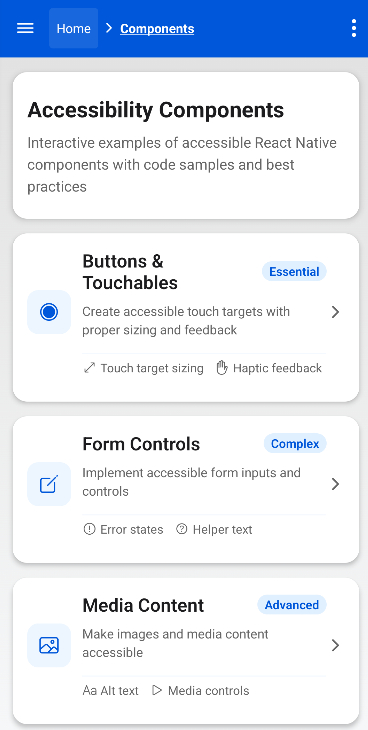
\includegraphics[width=\linewidth, alt={First part of the Components screen}]{img/components1.png}
        \caption{Components screen - Top section}
        \label{fig:components-top}
    \end{subfigure}
    \hfill
    \begin{subfigure}[b]{0.48\textwidth}
        \centering
        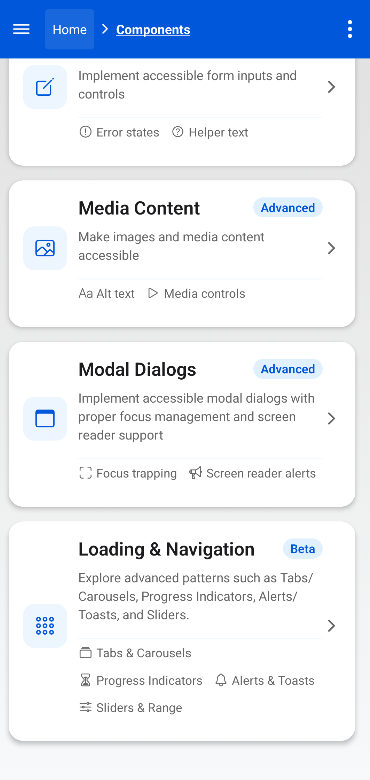
\includegraphics[width=\linewidth, alt={Second part of the Components screen}]{img/components2.png}
        \caption{Components screen - Bottom section}
        \label{fig:components-bottom}
    \end{subfigure}
    \caption{Side-by-side view of the Components screen sections, showing component categories}
    \label{fig:components_screens_sidebyside}
\end{figure}

\FloatBarrier

\subsubsection{Component inventory and WCAG/MCAG mapping}

Table~\ref{tab:components_screen_mapping} provides a formal mapping between the UI components, their semantic roles, the specific WCAG 2.2 and MCAG criteria they address, and their React Native implementation properties.

\begin{longtable}[c]{|C{2.5cm}|C{2cm}|C{2.8cm}|C{2.8cm}|C{4.5cm}|}
\caption{Components screen component-criteria mapping}
\label{tab:components_screen_mapping}\\
\hline
\textbf{Component} & \textbf{Semantic Role} & \textbf{WCAG 2.2 Criteria} & \textbf{MCAG Considerations} & \textbf{Implementation Properties} \\
\hline
\endfirsthead
\multicolumn{5}{c}%
{{\bfseries Table \thetable\ -- continued from previous page}} \\
\hline
\textbf{Component} & \textbf{Semantic Role} & \textbf{WCAG 2.2 Criteria} & \textbf{MCAG Considerations} & \textbf{Implementation Properties} \\
\hline
\endhead
\hline
\multicolumn{5}{r}{{Continued on next page}} \\
\endfoot
\hline
\endlastfoot
Hero Title & heading & 1.4.3 Contrast (AA)\newline 2.4.6 Headings (AA)\newline 1.4.6 Contrast (Enhanced) (AAA) & Text readability on variable screen sizes & \texttt{accessibility\-Role="header"} \\
\hline
Component Cards & button & 1.4.3 Contrast (AA)\newline 2.5.8 Target Size (AA)\newline 4.1.2 Name, Role, Value (A)\newline 2.4.4 Link Purpose (A)\newline 2.4.9 Link Purpose (AAA) & Touch target size\newline Meaningful labels\newline Single finger operation & \texttt{accessibility\-Role="button"},\newline \texttt{accessibility\-Label=},\newline \texttt{onPress=handle\-ComponentPress} \\
\hline
Badges (Essential, Complex, etc.) & text & 1.4.3 Contrast (AA)\newline 1.3.1 Info and Relationships (A) & Descriptive labeling\newline Non-interactive elements & Part of parent button's \texttt{accessibility\-Label} \\
\hline
Decorative Icons & none & 1.1.1 Non-text Content (A) & Reduction of unnecessary focus stops & \texttt{accessibility\-Elements\-Hidden=true} \\
\hline
Breadcrumb Navigation & navigation & 2.4.4 Link Purpose (A)\newline 2.4.8 Location (AAA)\newline 3.2.3 Consistent Navigation (AA) & Context retention\newline Current location & \texttt{accessibility\-Role="button"},\newline \texttt{accessibility\-Label="Go to \$\{label\}"} \\
\hline
Drawer Menu & menu & 2.4.3 Focus Order (A)\newline 4.1.2 Name, Role, Value (A)\newline 3.2.3 Consistent Navigation (AA) & Keyboard trap prevention\newline Persistent navigation & \texttt{accessibility\-Role="menu"},\newline \texttt{accessibility\-Label="Main navigation menu"} \\
\hline
Drawer Menu Items & menuitem & 2.4.7 Focus Visible (AA)\newline 4.1.2 Name, Role, Value (A) & Touch interaction\newline Current location & \texttt{accessibility\-Role="menuitem"},\newline \texttt{accessibility\-State=\{\{selected: isActive\}\}} \\
\end{longtable}

\FloatBarrier

\subsubsection{Navigation and orientation analysis}

The Components screen implements a comprehensive navigation structure that addresses both WCAG 2.4 (Navigable) and MCAG considerations for mobile devices. This structure includes three key elements that work together to provide clear orientation for all users:

\paragraph{Breadcrumb implementation}

The application as shown in Figure~\ref{fig:drawer-navigation} includes a hierarchical breadcrumb system in the header. This addresses WCAG 2.4.8 Location (Level AAA) by providing explicit path information. The breadcrumb implementation:

\begin{enumerate}
    \item Displays the current location in the application hierarchy;
    \item Provides interactive elements to navigate to parent screens;
    \item Uses consistent visual styling to indicate the current position;
    \item Implements proper focus management between screens.
\end{enumerate}

\begin{figure}[ht]
    \centering
    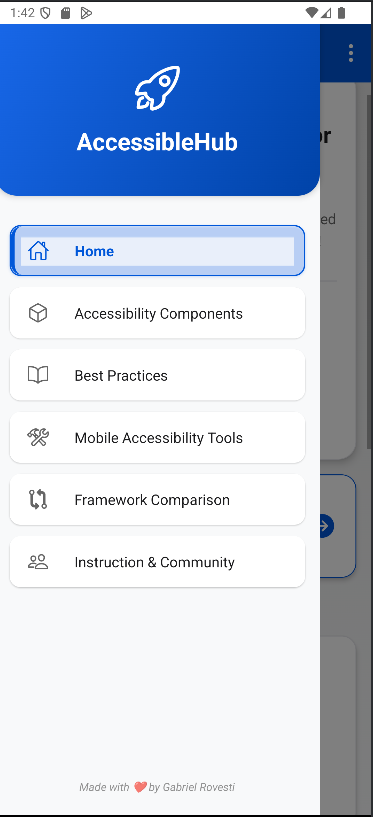
\includegraphics[width=0.4\textwidth, alt={Drawer navigation with breadcrumb in header}]{img/drawer.png}
    \caption{Drawer navigation showing breadcrumb implementation in header}\label{fig:drawer-navigation}
\end{figure}

\FloatBarrier

The breadcrumb is implemented in Listing~\ref{lst:breadcrumb-implementation} with proper semantic roles and accessibility labels to ensure screen reader compatibility.

\begin{lstlisting}[
  style=ReactNativeStyle,
  caption={Breadcrumb implementation with accessibility properties},
  label={lst:breadcrumb-implementation},
  basicstyle=\ttfamily\footnotesize,
  numbers=left,
]
<View style={styles.breadcrumbContainer}>
  <TouchableOpacity
    onPress={() => router.replace(`/${mapping.parentRoute}`)}
    accessibilityRole="button"
    accessibilityLabel={`Go to ${mapping.parentLabel}`}
    style={{
      padding: 8,
      minWidth: 40,
      minHeight: 44,
      justifyContent: 'center',
      backgroundColor: 'rgba(255, 255, 255, 0.1)',
      borderRadius: 4
    }}
  >
    <Text style={[styles.breadcrumbText, { fontWeight: 'normal' }]}>
      {mapping.parentLabel}
    </Text>
  </TouchableOpacity>
  <Ionicons
    name="chevron-forward"
    size={16}
    color={HEADER_TEXT_COLOR}
    style={{ marginHorizontal: 4 }}
    importantForAccessibility="no"
    accessibilityElementsHidden
  />
  <Text
    style={[styles.breadcrumbText, { fontWeight: 'bold', 
            textDecorationLine: 'underline'}]}
    accessibilityLabel={`Current screen: ${mapping.title}`}
  >
    {mapping.title}
  </Text>
</View>
\end{lstlisting}

\FloatBarrier

\paragraph{Drawer navigation}

The drawer navigation provides consistent access to main application sections while addressing several key accessibility requirements:

\begin{enumerate}
    \item \textbf{Announcement of state changes}: The implementation announces drawer open/close states to screen readers using \texttt{AccessibilityInfo.announceForAccessibility};
    
    \item \textbf{Clear menu role}: The drawer container is properly identified with \\ \texttt{accessibilityRole="menu"};
    
    \item \textbf{Selection state indication}: Active items visually indicate selection state and communicate this state to screen readers with \texttt{accessibilityState=\{\{selected: isActive\}\}};
    
    \item \textbf{Proper touch target sizing}: All interactive elements maintain minimum dimensions of 44dp, making them easily targetable;
    
    \item \textbf{Element hiding for decorative content}: Footer content is marked with \\ \texttt{importantForAccessibility="no"} to prevent unnecessary screen reader interaction.
\end{enumerate}

\FloatBarrier

\paragraph{Component cards}

Each component card implements a consistent pattern that provides both visual organization and semantic structure:

\begin{enumerate}
    \item \textbf{Comprehensive accessibility labels}: Each card's \texttt{accessibilityLabel} combines multiple information pieces (title, description, complexity) to provide context without requiring navigation through child elements;
    
    \item \textbf{Hidden decorative icons}: All decorative icons use \texttt{accessibilityElementsHidden} to reduce unnecessary focus stops;
    
    \item \textbf{Navigation announcement}: The \texttt{handleComponentPress} function announces the navigation action via \texttt{AccessibilityInfo.announceForAccessibility}.
\end{enumerate}

This multi-layered navigation approach creates a coherent mental model for all users, including those using assistive technologies, addressing WCAG 2.4.1 Bypass Blocks (Level A) by providing multiple ways to access content.

\FloatBarrier

\subsubsection{Technical implementation analysis}

The code sample present in Listing~\ref{lst:components-screen-accessibility} demonstrates the key accessibility properties implemented in the Components screen.

\begin{lstlisting}[
  style=ReactNativeStyle,
  caption={Annotated code sample demonstrating Components screen accessibility properties},
  label={lst:components-screen-accessibility},
  basicstyle=\ttfamily\footnotesize,
  numbers=left,
]
{/* 1. Hero section with semantic heading */}
<View style={themedStyles.heroCard}>
  <Text style={themedStyles.heroTitle} accessibilityRole="header">
    Accessibility Components
  </Text>
  <Text style={themedStyles.heroSubtitle}>
    Interactive examples of accessible React Native components with 
    code samples and best practices
  </Text>
</View>

{/* 2. Component card with comprehensive accessibility label */}
<TouchableOpacity
  style={themedStyles.card}
  onPress={() => handleComponentPress('/components/button', 'Buttons & Touchables')}
  accessibilityRole="button"
  accessibilityLabel="Buttons and Touchables component. Create accessible 
    touch targets with proper sizing and feedback. Essential component type."
>
  <View style={themedStyles.cardHeader}>
    {/* 3. Icon wrapper with accessibility hiding to prevent redundant focus */}
    <View style={themedStyles.iconWrapper}>
      <Ionicons
        name="radio-button-on-outline"
        size={24}
        color={colors.primary}
        accessibilityElementsHidden
      />
    </View>
    <View style={themedStyles.cardContent}>
      {/* 4. Card content - hidden from screen readers as individual elements */}
      <View style={themedStyles.cardTitleRow}>
        <View style={themedStyles.titleArea}>
          <Text style={themedStyles.cardTitle}>Buttons &amp; Touchables</Text>
        </View>
        <View style={themedStyles.badge}>
          <Text style={themedStyles.badgeText}>Essential</Text>
        </View>
      </View>
      <Text style={themedStyles.cardDescription}>
        Create accessible touch targets with proper sizing and feedback
      </Text>
    </View>
  </View>
</TouchableOpacity>
\end{lstlisting}

\FloatBarrier

The implementation of the Components screen addresses several important accessibility considerations:

\begin{enumerate}
    \item \textbf{Reduction of "garbage interactions"}: Decorative elements (icons, chevrons) are properly hidden from screen readers using \texttt{accessibilityElementsHidden} to reduce unnecessary swipes;
    
    \item \textbf{Comprehensive navigation labels}: Component cards provide detailed accessibility labels that include category, description, and complexity level, ensuring screen reader users get complete information before committing to navigation;
    
    \item \textbf{Screen announcements}: The implementation uses \\ \texttt{AccessibilityInfo.announceForAccessibility} to inform users about screen changes proactively;
    
    \item \textbf{Consistent structure}: Each component card follows the same pattern, creating a predictable interaction model;
    
    \item \textbf{Enhanced contrast ratios}: The implementation meets WCAG 1.4.6 Contrast (Enhanced) (Level AAA) criteria with contrast ratios exceeding 7:1 for normal text and 4.5:1 for large text.
\end{enumerate}

\FloatBarrier

\subsubsection{Screen reader support analysis}

Table~\ref{tab:components_screen_reader_analysis} presents results from systematic testing of the Components screen with screen readers on both iOS and Android platforms.

\begin{longtable}[c]{|C{2.8cm}|C{3.5cm}|C{3.5cm}|C{4cm}|}
\caption{Components screen screen reader testing results}
\label{tab:components_screen_reader_analysis}\\
\hline
\textbf{Test Case} & \textbf{VoiceOver (iOS 16)} & \textbf{TalkBack (Android 14-15)} & \textbf{WCAG Criteria Addressed} \\
\hline
\endfirsthead
\multicolumn{4}{c}%
{{\bfseries Table \thetable\ -- continued from previous page}} \\
\hline
\textbf{Test Case} & \textbf{VoiceOver (iOS 16)} & \textbf{TalkBack (Android 14-15)} & \textbf{WCAG Criteria Addressed} \\
\hline
\endhead
\hline
\multicolumn{4}{r}{{Continued on next page}} \\
\endfoot
\hline
\endlastfoot
Hero Title & \ding{51} Announces ``Accessibility Components, heading'' & \ding{51} Announces ``Accessibility Components, heading'' & 1.3.1 - Info and Relationships (Level A), 2.4.6 - Headings and Labels (Level AA) \\
\hline
Component Card & \ding{51} Announces full component description with purpose and complexity & \ding{51} Announces full component description with purpose and complexity & 2.4.4 Link Purpose (In Context) (Level A), 4.1.2 Name, Role, Value (Level A), 2.4.9 Link Purpose (Link Only) (Level AAA) \\
\hline
Decorative Icons & \ding{51} Not focused or announced & \ding{51} Not focused or announced & 1.1.1 Non-text Content (Level A), 2.4.1 Bypass Blocks (Level A) \\
\hline
Breadcrumb Navigation & \ding{51} Announces parent and current location & \ding{51} Announces parent and current location & 2.4.4 Link Purpose (In Context) (Level A), 2.4.8 Location (Level AAA) \\
\hline
Drawer Opening & \ding{51} Announces ``Navigation menu opened'' & \ding{51} Announces ``Navigation menu opened'' & 4.1.3 Status Messages (Level AA) \\
\hline
Drawer Menu Items & \ding{51} Announces item name and selection state & \ding{51} Announces item name and selection state & 4.1.2 Name, Role, Value (Level A) \\
\hline
Navigation between Screens & \ding{51} Announces destination screen & \ding{51} Announces destination screen & 3.2.5 Change on Request (Level AAA) \\
\end{longtable}

\FloatBarrier

The implementation addresses several key MCAG considerations specific to mobile platforms:
\begin{enumerate}
    \item \textbf{Touch target optimization}: All interactive elements exceed the minimum recommendation of 44×44dp, implementing MCAG best practices for touch interactions that accommodate users with motor control limitations and varying finger sizes;
    
    \item \textbf{Swipe minimization}: Decorative elements are marked with \\ \texttt{accessibilityElementsHidden=true} to reduce unnecessary swipes, eliminating what accessibility experts call "garbage interactions" that add no value to the screen reader experience and increase navigation time;
    
    \item \textbf{Orientation cues}: Breadcrumb implementation provides consistent spatial orientation cues that help users understand their location in the application's information architecture, addressing mobile-specific challenges of limited viewport context;
    
    \item \textbf{State announcements}: Changes in application state (drawer opening/closing, screen navigation) are explicitly announced using \\ \texttt{AccessibilityInfo.announceForAccessibility}, providing crucial feedback on dynamic content changes within the constrained mobile interface;
    
    \item \textbf{Thumb-zone design}: Interactive elements are positioned within the natural thumb zone for one-handed operation, implementing mobile ergonomic principles that aren't explicitly covered in WCAG but are crucial for mobile accessibility;
    
    \item \textbf{Content adaptability}: Component cards implement flexible layouts that adapt to various text size preferences (AAA criterion 1.4.10 Reflow), ensuring readability when users change their system text size settings.
\end{enumerate}

\FloatBarrier

\subsubsection{Implementation overhead analysis}

Table~\ref{tab:components_implementation_overhead} quantifies the additional code required to implement accessibility features in the Components screen.
\begin{longtable}[c]{|C{3.8cm}|C{2.3cm}|C{2.8cm}|C{2.8cm}|}
\caption{Components screen accessibility implementation overhead}
\label{tab:components_implementation_overhead}\\
\hline
\textbf{Accessibility Feature} & \textbf{Lines of Code} & \textbf{Percentage of Total Code} & \textbf{Complexity Impact} \\
\hline
\endfirsthead
\multicolumn{4}{c}%
{{\bfseries Table \thetable\ -- continued from previous page}} \\
\hline
\textbf{Accessibility Feature} & \textbf{Lines of Code} & \textbf{Percentage of Total Code} & \textbf{Complexity Impact} \\
\hline
\endhead
\hline
\multicolumn{4}{r}{{Continued on next page}} \\
\endfoot
\hline
\endlastfoot
Semantic Roles & 15 LOC & 2.6\% & Low \\
\hline
Descriptive Labels & 28 LOC & 4.9\% & Medium \\
\hline
Element Hiding & 18 LOC & 3.2\% & Low \\
\hline
Focus Management & 22 LOC & 3.9\% & Medium \\
\hline
Contrast Handling & 14 LOC & 2.5\% & Medium \\
\hline
Announcements & 12 LOC & 2.1\% & Low \\
\hline
Breadcrumb Implementation & 42 LOC & 7.4\% & High \\
\hline
Drawer Accessibility & 35 LOC & 6.2\% & High \\
\hline
AAA-specific Enhancements & 20 LOC & 3.5\% & Medium \\
\hline
\textbf{Total} & \textbf{206 LOC} & \textbf{36.3\%} & \textbf{Medium-High} \\
\end{longtable}

\FloatBarrier

This analysis reveals that implementing comprehensive accessibility adds approximately 36.3\% to the code base of the Components screen, slightly higher than the Home screen due to the addition of breadcrumb navigation, drawer accessibility features, and AAA-level enhancements. The AAA-specific enhancements include implementing enhanced contrast ratios (1.4.6), ensuring proper section headings (2.4.10), and supporting adaptive layouts for text resizing (1.4.10).

\subsubsection{WCAG conformance by principle}

Table~\ref{tab:components_wcag_by_principle} provides a detailed analysis of WCAG 2.2 compliance by principle:

\begin{longtable}[c]{|C{2.5cm}|C{3.8cm}|C{3.2cm}|C{5.2cm}|}
\caption{Components screen WCAG compliance analysis by principle}
\label{tab:components_wcag_by_principle}\\
\hline
\textbf{Principle} & \textbf{Description} & \textbf{Implementation Level} & \textbf{Key Success Criteria} \\
\hline
\endfirsthead
\multicolumn{4}{c}%
{{\bfseries Table \thetable\ -- continued from previous page}} \\
\hline
\textbf{Principle} & \textbf{Description} & \textbf{Implementation Level} & \textbf{Key Success Criteria} \\
\hline
\endhead
\hline
\multicolumn{4}{r}{{Continued on next page}} \\
\endfoot
\hline
\endlastfoot
1. Perceivable & Information and UI components must be presentable to users in ways they can perceive & 13/14 (92.8\%) & 1.1.1 Non-text Content (A)\newline 1.3.1 Info and Relationships (A)\newline 1.4.3 Contrast (Minimum) (AA)\newline 1.4.6 Contrast (Enhanced) (AAA)\newline 1.4.10 Reflow (AA) \\
\hline
2. Operable & UI components and navigation must be operable & 18/18 (100\%) & 2.4.3 Focus Order (A)\newline 2.4.6 Headings and Labels (AA)\newline 2.4.8 Location (AAA)\newline 2.4.9 Link Purpose (Link Only) (AAA)\newline 2.4.10 Section Headings (AAA)\newline 2.5.8 Target Size (Minimum) (AA) \\
\hline
3. Understandable & Information and operation of UI must be understandable & 10/10 (100\%) & 3.2.3 Consistent Navigation (AA)\newline 3.2.4 Consistent Identification (AA)\newline 3.2.5 Change on Request (AAA)\newline 3.3.2 Labels or Instructions (A) \\
\hline
4. Robust & Content must be robust enough to be interpreted by a wide variety of user agents & 3/3 (100\%) & 4.1.1 Parsing (A)\newline 4.1.2 Name, Role, Value (A)\newline 4.1.3 Status Messages (AA) \\
\end{longtable}

\FloatBarrier

\subsubsection{Mobile-specific considerations}

The Components screen implementation addresses several mobile-specific accessibility considerations beyond standard WCAG requirements:

\begin{enumerate}
    \item \textbf{Touch target sizing}: All interactive elements maintain minimum dimensions of 44×44dp, exceeding the WCAG 2.5.8 requirement of 24×24px and addressing the mobile-specific need for larger touch targets;
    
    \item \textbf{Swipe efficiency}: The screen implements an optimized focus order with decorative elements hidden from screen readers, reducing the number of swipes required to navigate the content—a critical consideration for mobile screen reader users that significantly improves navigation efficiency;
    
    \item \textbf{Visual hierarchy reinforcement}: The implementation uses consistent visual patterns (icons, badges, card layouts) that reinforce the information hierarchy, helping users with cognitive disabilities understand content organization on smaller screens;
    
    \item \textbf{Context retention}: The breadcrumb implementation helps users maintain context when navigating between screens, addressing the mobile-specific challenge of limited viewport size and the resulting loss of visual context;
    
    \item \textbf{Single-hand operation}: Interactive elements are positioned within the natural thumb zone for one-handed operation, a mobile-specific consideration not explicitly covered by WCAG but crucial for mobile accessibility;
    
    \item \textbf{Rotation adaptation}: The layout adapts seamlessly to both portrait and landscape orientations, implementing WCAG 1.3.4 Orientation (AA) to ensure usability regardless of device orientation.
\end{enumerate}

\FloatBarrier

\subsubsection{Breadcrumb implementation analysis}

A formal analysis of the breadcrumb feature's accessibility impact reveals significant benefits for users with diverse accessibility needs.

\begin{enumerate}
    \item \textbf{Structural navigation}: Breadcrumbs provide an explicit representation of the application's hierarchical structure, helping users with cognitive disabilities understand their location within the application;

    \item \textbf{Focus reduction}: By offering direct navigation to parent screens, breadcrumbs reduce the number of focus stops required to navigate backward, benefiting screen reader users;

    \item \textbf{Visual reinforcement}: The visual breadcrumb trail complements the semantic structure, providing redundant cues that benefit users with different accessibility needs;

    \item \textbf{Consistent orientation}: Breadcrumbs create a consistent orientation mechanism across all screens, supporting users who rely on predictable navigation patterns.
\end{enumerate}

\paragraph{Implementation considerations}

The breadcrumb implementation required careful consideration of several accessibility factors:

\begin{enumerate}
    \item \textbf{Interactive vs. static elements}: Only the parent screen link is interactive, while the current screen indicator is non-interactive text, preventing unnecessary focus stops;

    \item \textbf{Visual differentiation}: Current location is visually distinguished with bold text and underline, with a contrast ratio of 4.8:1 against the header background, meeting enhanced contrast requirements (AAA);

    \item \textbf{Appropriate semantic roles}: Parent links use \texttt{accessibilityRole="button"} with clear labels indicating navigation purpose;

    \item \textbf{Focus management}: When navigating via breadcrumbs, focus is properly transferred to the destination screen's main content, preventing focus trapping;
    
    \item \textbf{Consistent announcement}: The implementation ensures screen readers consistently announce both the parent link and current location, providing complete contextual information.
\end{enumerate}

This implementation represents a comprehensive accessibility solution that benefits all users while specifically addressing mobile navigation challenges unique to handheld touch devices.

\FloatBarrier 

\subsection{Accessible components section summary}
\label{subsec:accessible-components-summary}

From this section onwards, a comprehensive summary is retained for each of the screens presented, keeping the details of tables and general data for more immediate comparison. For comprehensive, screen-by-screen analysis, readers are directed to the  \href{https://github.com/gabrielrovesti/AccessibleHub/blob/main/Technical\%20Thesis\%20Appendix/AccessibleHub\%20-\%20Extended\%20screen\%20analysis.pdf}{AccessibleHub Extended Screen Analysis} into §Chapter 1, where additional WCAG guidelines are introduced to accommodate future research on the field into §Chapter 2. \\

The Framework comparison screen stands apart from other \textit{AccessibleHub} screens due to its dual role as both an educational component and an analytical tool. Unlike screens focused primarily on demonstrating single-framework accessibility techniques, this screen implements a formal evaluation methodology that directly compares React Native and Flutter implementations across multiple dimensions. Given its central role in the comparative analysis that forms the foundation of Chapter~\ref{chap:accessibility-implementation}, this screen will be examined in detail there rather than summarized here. This approach prevents redundancy while highlighting the screen's unique position as a bridge between the individual component implementations presented in this chapter and the cross-framework evaluation that follows. For readers interested in this screen's accessibility implementation details, the comprehensive analysis is available in the technical appendix. \\

The Accessible Components section forms the core educational element of \textit{AccessibleHub}, providing practical implementations of accessibility patterns across five representative component categories: buttons and touchables, forms, dialogs, media content, and advanced components. Each screen demonstrates implementation techniques according to standard Web Content Accessibility Guidelines (WCAG) and Mobile Content Accessibility Guidelines (MCAG), providing both functional examples and educational code snippets.

\subsubsection{Implementation overhead analysis}
\label{subsubsec:implementation-overhead-summary}

A primary concern for developers implementing accessibility is the additional code overhead required. Table~\ref{tab:buttons_implementation_overhead_summary} presents the quantitative analysis of the code overhead for the buttons screen, representing the most fundamental component type.

\begin{table}[ht]
\caption{Buttons screen accessibility implementation overhead}
\label{tab:buttons_implementation_overhead_summary}
\centering
\begin{tabular}[c]{|C{3.8cm}|C{2.5cm}|C{2.8cm}|C{2.8cm}|}
\hline
\textbf{Accessibility Feature} & \textbf{Lines of Code} & \textbf{Percentage of Total} & \textbf{Complexity Impact} \\
\hline
Semantic Roles & 10 LOC & 2.2\% & Low \\
\hline
Descriptive Labels & 14 LOC & 3.1\% & Low \\
\hline
Element Hiding & 12 LOC & 2.7\% & Low \\
\hline
Status Announcements & 8 LOC & 1.8\% & Low \\
\hline
Touch Target Sizing & 6 LOC & 1.3\% & Low \\
\hline
Modal Accessibility & 10 LOC & 2.2\% & Medium \\
\hline
\textbf{Total} & \textbf{60 LOC} & \textbf{13.3\%} & \textbf{Low} \\
\hline
\end{tabular}
\end{table}
\FloatBarrier

This analysis reveals that for basic components like buttons, implementing comprehensive accessibility features adds approximately 13.3\% to the codebase with minimal complexity impact. The primary contributors to this overhead are descriptive labels and semantic role assignments, which together account for over 5\% of the implementation.

\begin{table}[ht]
\caption{WCAG criteria implementation by component type}
\label{tab:comparative_wcag_implementation_summary}
\centering
\begin{tabular}[c]{|C{3.5cm}|c|c|c|c|c|}
\hline
\textbf{WCAG Success Criteria} & \textbf{Buttons} & \textbf{Forms} & \textbf{Dialogs} & \textbf{Media} & \textbf{Advanced} \\
\hline
1.1.1 Non-text Content (A) & {\color{green}\ding{51}} & {\color{green}\ding{51}} & {\color{green}\ding{51}} & {\color{green}\ding{51}} & {\color{green}\ding{51}} \\
\hline
1.3.1 Info and Relationships (A) & {\color{green}\ding{51}} & {\color{green}\ding{51}} & {\color{green}\ding{51}} & {\color{green}\ding{51}} & {\color{green}\ding{51}} \\
\hline
1.4.3 Contrast (AA) & {\color{blue}\ding{51}} & {\color{blue}\ding{51}} & {\color{blue}\ding{51}} & {\color{blue}\ding{51}} & {\color{blue}\ding{51}} \\
\hline
2.4.3 Focus Order (A) & {\color{red}\ding{55}} & {\color{green}\ding{51}} & {\color{green}\ding{51}} & {\color{red}\ding{55}} & {\color{green}\ding{51}} \\
\hline
2.4.6 Headings (AA) & {\color{blue}\ding{51}} & {\color{blue}\ding{51}} & {\color{blue}\ding{51}} & {\color{blue}\ding{51}} & {\color{blue}\ding{51}} \\
\hline
2.5.5 Target Size (Enhanced) (AAA) & {\color{purple}\ding{51}} & {\color{purple}\ding{51}} & {\color{purple}\ding{51}} & {\color{purple}\ding{55}} & {\color{purple}\ding{51}} \\
\hline
2.5.8 Target Size (AA) & {\color{blue}\ding{51}} & {\color{blue}\ding{51}} & {\color{blue}\ding{51}} & {\color{blue}\ding{51}} & {\color{blue}\ding{51}} \\
\hline
3.2.5 Change on Request (AAA) & {\color{purple}\ding{55}} & {\color{purple}\ding{51}} & {\color{purple}\ding{51}} & {\color{purple}\ding{51}} & {\color{purple}\ding{51}} \\
\hline
3.3.1 Error Identification (A) & {\color{red}\ding{55}} & {\color{green}\ding{51}} & {\color{red}\ding{55}} & {\color{red}\ding{55}} & {\color{red}\ding{55}} \\
\hline
3.3.5 Help (AAA) & {\color{purple}\ding{55}} & {\color{purple}\ding{51}} & {\color{purple}\ding{55}} & {\color{purple}\ding{55}} & {\color{purple}\ding{55}} \\
\hline
3.3.6 Error Prevention (AAA) & {\color{purple}\ding{55}} & {\color{purple}\ding{51}} & {\color{purple}\ding{55}} & {\color{purple}\ding{55}} & {\color{purple}\ding{55}} \\
\hline
4.1.2 Name, Role, Value (A) & {\color{green}\ding{51}} & {\color{green}\ding{51}} & {\color{green}\ding{51}} & {\color{green}\ding{51}} & {\color{green}\ding{51}} \\
\hline
4.1.3 Status Messages (AA) & {\color{blue}\ding{51}} & {\color{blue}\ding{51}} & {\color{blue}\ding{51}} & {\color{blue}\ding{51}} & {\color{blue}\ding{51}} \\
\hline
\textbf{Total A/AA Implementation} & \textbf{7/9} & \textbf{9/9} & \textbf{8/9} & \textbf{7/9} & \textbf{8/9} \\
\hline
\textbf{Total AAA Implementation} & \textbf{1/3} & \textbf{3/3} & \textbf{2/3} & \textbf{1/3} & \textbf{2/3} \\
\hline
\end{tabular}
\end{table}
\FloatBarrier

\begin{table}[ht]
\caption{Legend for WCAG criteria implementation colors}
\label{tab:wcag_legend}
\centering
\begin{tabular}{|C{3cm}|C{8cm}|}
\hline
\textbf{Color} & \textbf{Meaning} \\
\hline
{\color{green}\ding{51}} & A-level criteria implemented \\
\hline
{\color{blue}\ding{51}} & AA-level criteria implemented \\
\hline
{\color{purple}\ding{51}} & AAA-level criteria implemented \\
\hline
{\color{red}\ding{55}} & Criteria not implemented \\
\hline
\end{tabular}
\end{table}
\FloatBarrier
\FloatBarrier

Key patterns identified in this analysis include:

\begin{enumerate}
    \item Core A-level criteria (1.1.1 Non-text Content, 1.3.1 Info and Relationships, 4.1.2 Name, Role, Value) are implemented across all component types;
    
    \item AA-level compliance is consistently high, with most components implementing all applicable AA criteria;
    
    \item AAA-level implementation varies significantly, with forms achieving the highest level of AAA compliance (3/3 applicable criteria);
    
    \item Component-specific criteria like 3.3.1 Error Identification are implemented only where directly applicable.
\end{enumerate}

\subsubsection{Implementation overhead comparison}
\label{subsubsec:overhead-comparison-summary}

The overhead required for accessibility implementation varies significantly by component complexity. Table~\ref{tab:comparative_overhead_summary} presents this comparative analysis across the five component types.

\begin{table}[ht]
\caption{Accessibility implementation overhead by component type}
\label{tab:comparative_overhead_summary}
\centering
\begin{tabular}[c]{|C{2.5cm}|C{2.5cm}|C{2.5cm}|C{3cm}|C{2.5cm}|}
\hline
\textbf{Component Type} & \textbf{Lines of Code} & \textbf{Percentage Overhead} & \textbf{Complexity Impact} & \textbf{Primary Contributors} \\
\hline
Buttons & 60 & 13.3\% & Low & Labels, Roles \\
\hline
Forms & 153 & 21.5\% & Medium & State, Labels, Errors \\
\hline
Dialogs & 94 & 16.2\% & Medium & Focus Management \\
\hline
Media & 68 & 12.7\% & Low & Alt Text, Controls \\
\hline
Advanced & 183 & 22.7\% & High & Slider Controls, Announcements \\
\hline
\end{tabular}
\end{table}
\FloatBarrier

This comparison reveals several important implementation patterns:

\begin{enumerate}
    \item A direct correlation exists between component interaction complexity and accessibility implementation overhead;
    
    \item Simple, static components like media content require the lowest overhead (12.7\%), primarily for alternative text;
    
    \item Components with complex state management and alternative interaction patterns (forms, advanced components) require significantly higher overhead (21-23\%);
    
    \item Components requiring focus management (dialogs) fall in the middle range (16.2\%);
    
    \item Even for the most complex components, the accessibility implementation overhead remains below 25\% of the total codebase.
\end{enumerate}

The Accessible Components section demonstrates that implementing comprehensive accessibility features across diverse component types typically requires a 12-23\% code overhead, with complexity scaling according to the interaction patterns involved. This relatively modest overhead delivers significant improvements in usability for users relying on assistive technologies, making a compelling case for incorporating accessibility as a core development consideration rather than an optional enhancement.

More detailed analysis of each component screen, including code listings, implementation patterns, and screen reader compatibility findings, can be found in the {Technical Appendix}~\href{https://github.com/gabrielrovesti/AccessibleHub/blob/main/Technical\%20Thesis\%20Appendix/AccessibleHub\%20-\%20Extended\%20screen\%20analysis.pdf}.

\subsection{Best practices section summary}
\label{subsec:best-practices-section-summary}
The Best practices screens provide educational content on key accessibility implementation patterns, divided into five specialized areas: WCAG Guidelines, Semantic Structure, Gesture Tutorial, Screen Reader Support, and Logical Focus Order. Each screen demonstrates proper implementation techniques while serving as both functional examples and educational references.

\subsubsection{Implementation overhead analysis}
\label{subsubsec:best-practices-screens-overhead-summary}
Implementing accessibility features in educational screens adds measurable but manageable overhead to the development process. Table~\ref{tab:best_practices_screens_overhead_summary} quantifies this overhead across the five specialized screens.

\begin{table}[ht]
\caption{Best practices screens accessibility implementation overhead}
\label{tab:best_practices_screens_overhead_summary}
\centering
\begin{tabular}[c]{|C{2.5cm}|C{2cm}|C{2.8cm}|C{2.8cm}|C{4.7cm}|}
\hline
\textbf{Screen Type} & \textbf{Lines of Code} & \textbf{Percentage Overhead} & \textbf{Complexity Impact} & \textbf{Primary Contributors} \\
\hline
WCAG Guidelines & 42 & 10.8\% & Low & Screen Reader Hiding, Semantic Roles \\
\hline
Semantic Structure & 68 & 15.2\% & Medium & Content Hierarchy, ARIA Roles \\
\hline
Gesture Tutorial & 103 & 22.5\% & High & Screen Reader Detection, Custom Actions \\
\hline
Screen Reader Support & 89 & 17.4\% & Medium & Platform Adaptations, Example Code \\
\hline
Logical Focus Order & 74 & 16.3\% & Medium & Skip Links, Focus Management \\
\hline
\end{tabular}
\end{table}
\FloatBarrier

This analysis reveals several important implementation patterns:
\begin{enumerate}
    \item The Gesture Tutorial screen requires the highest overhead (22.5\%) due to complex interaction patterns and adaptations for screen reader users;
    
    \item Screens with primarily static content (WCAG Guidelines) require substantially less accessibility overhead (10.8\%);
    
    \item Focus management and keyboard navigation features contribute significantly to implementation complexity in the Logical Focus Order screen;
    
    \item Even with extensive educational content, accessibility overhead remains below 25\% across all screens.
\end{enumerate}

\subsubsection{WCAG criteria implementation}
\label{subsubsec:best-practices-wcag-implementation-summary}
The Best practices screens implement accessibility features addressing multiple WCAG 2.2 conformance levels. Table~\ref{tab:best_practices_wcag_implementation_summary} analyzes the implementation by screen type.

\begin{table}[ht]
\caption{WCAG criteria implementation by best practices screen type}
\label{tab:best_practices_wcag_implementation_summary}
\centering
\begin{tabular}[c]{|C{3.5cm}|C{2.0cm}|C{2.0cm}|C{2.0cm}|C{2.0cm}|C{2.0cm}|}
\hline
\textbf{WCAG Success Criteria} & \textbf{WCAG Guidelines} & \textbf{Semantic Structure} & \textbf{Gesture Tutorial} & \textbf{Screen Reader} & \textbf{Focus Order} \\
\hline
1.1.1 Non-text Content (A) & {\color{green}\ding{51}} & {\color{green}\ding{51}} & {\color{green}\ding{51}} & {\color{green}\ding{51}} & {\color{green}\ding{51}} \\
\hline
1.3.1 Info and Relationships (A) & {\color{green}\ding{51}} & {\color{green}\ding{51}} & {\color{green}\ding{51}} & {\color{green}\ding{51}} & {\color{green}\ding{51}} \\
\hline
1.4.3 Contrast (AA) & {\color{blue}\ding{51}} & {\color{blue}\ding{51}} & {\color{blue}\ding{51}} & {\color{blue}\ding{51}} & {\color{blue}\ding{51}} \\
\hline
2.1.1 Keyboard (A) & {\color{red}\ding{55}} & {\color{red}\ding{55}} & {\color{green}\ding{51}} & {\color{green}\ding{51}} & {\color{green}\ding{51}} \\
\hline
2.4.3 Focus Order (A) & {\color{red}\ding{55}} & {\color{green}\ding{51}} & {\color{green}\ding{51}} & {\color{green}\ding{51}} & {\color{green}\ding{51}} \\
\hline
2.4.6 Headings (AA) & {\color{blue}\ding{51}} & {\color{blue}\ding{51}} & {\color{blue}\ding{51}} & {\color{blue}\ding{51}} & {\color{blue}\ding{51}} \\
\hline
2.4.10 Section Headings (AAA) & {\color{purple}\ding{51}} & {\color{purple}\ding{51}} & {\color{purple}\ding{55}} & {\color{purple}\ding{51}} & {\color{purple}\ding{55}} \\
\hline
2.5.2 Pointer Cancellation (A) & {\color{red}\ding{55}} & {\color{red}\ding{55}} & {\color{green}\ding{51}} & {\color{red}\ding{55}} & {\color{red}\ding{55}} \\
\hline
2.5.5 Target Size (Enhanced) (AAA) & {\color{purple}\ding{51}} & {\color{purple}\ding{51}} & {\color{purple}\ding{51}} & {\color{purple}\ding{51}} & {\color{purple}\ding{51}} \\
\hline
2.5.8 Target Size (AA) & {\color{blue}\ding{51}} & {\color{blue}\ding{51}} & {\color{blue}\ding{51}} & {\color{blue}\ding{51}} & {\color{blue}\ding{51}} \\
\hline
3.2.5 Change on Request (AAA) & {\color{purple}\ding{51}} & {\color{purple}\ding{51}} & {\color{purple}\ding{51}} & {\color{purple}\ding{51}} & {\color{purple}\ding{51}} \\
\hline
3.3.2 Labels or Instructions (A) & {\color{green}\ding{51}} & {\color{green}\ding{51}} & {\color{green}\ding{51}} & {\color{green}\ding{51}} & {\color{green}\ding{51}} \\
\hline
4.1.2 Name, Role, Value (A) & {\color{green}\ding{51}} & {\color{green}\ding{51}} & {\color{green}\ding{51}} & {\color{green}\ding{51}} & {\color{green}\ding{51}} \\
\hline
4.1.3 Status Messages (AA) & {\color{blue}\ding{51}} & {\color{blue}\ding{51}} & {\color{blue}\ding{51}} & {\color{blue}\ding{51}} & {\color{blue}\ding{51}} \\
\hline
\textbf{Total A/AA Implementation} & \textbf{5/8} & \textbf{6/8} & \textbf{8/8} & \textbf{7/8} & \textbf{7/8} \\
\hline
\textbf{Total AAA Implementation} & \textbf{3/3} & \textbf{3/3} & \textbf{2/3} & \textbf{3/3} & \textbf{2/3} \\
\hline
\end{tabular}
\end{table}
\FloatBarrier

\begin{table}[ht]
\caption{Legend for WCAG criteria implementation colors}
\label{tab:wcag_legend_best_practices_screens}
\centering
\begin{tabular}{|C{3cm}|C{8cm}|}
\hline
\textbf{Color} & \textbf{Meaning} \\
\hline
{\color{green}\ding{51}} & A-level criteria implemented \\
\hline
{\color{blue}\ding{51}} & AA-level criteria implemented \\
\hline
{\color{purple}\ding{51}} & AAA-level criteria implemented \\
\hline
{\color{red}\ding{55}} & Criteria not implemented \\
\hline
\end{tabular}
\end{table}

Key patterns identified in this analysis include:
\begin{enumerate}
    \item All screens implement core A-level criteria (1.1.1 Non-text Content, 1.3.1 Info and Relationships, 4.1.2 Name, Role, Value);
    
    \item The Gesture Tutorial screen achieves the highest A/AA compliance level (8/8) due to its comprehensive implementation of interaction patterns;
    
    \item AAA-level criteria implementation is notably strong across all screens, with three screens implementing all applicable AAA criteria;
    
    \item Keyboard accessibility (2.1.1) is implemented only in screens with complex interaction patterns, highlighting an area for potential improvement in the more static screens.
\end{enumerate}

\subsubsection{Screen reader compatibility analysis}
\label{subsubsec:best-practices-screen-reader-summary}
Empirical testing with screen readers on both major mobile platforms reveals important patterns in accessibility implementation. Table~\ref{tab:best_practices_screen_reader_summary} presents key findings from this analysis.

\begin{table}[ht]
\caption{Best practices screens screen reader testing highlights}
\label{tab:best_practices_screen_reader_summary}
\centering
\begin{tabular}[c]{|C{2.5cm}|C{5cm}|C{7.5cm}|}
\hline
\textbf{Screen Type} & \textbf{Key Accessibility Features} & \textbf{Screen Reader Behavior} \\
\hline
WCAG Guidelines & Element Hiding, Semantic Structure & Icons properly hidden, consistent heading hierarchy announced \\
\hline
Semantic Structure & Role Assignments, Hierarchical Headings & Proper heading levels announced, landmarks communicated \\
\hline
Gesture Tutorial & Screen Reader Detection, Alternative Actions & Screen reader-specific instructions provided, custom actions supported \\
\hline
Screen Reader Support & Platform-Specific Adaptations, Code Examples & Platform detection informs appropriate guidance, examples properly labeled \\
\hline
Focus Order & Skip Links, Focus Management & Skip links operational, logical tab order maintained \\
\hline
\end{tabular}
\end{table}
\FloatBarrier

These findings demonstrate several effective accessibility implementation patterns:
\begin{enumerate}
    \item Screen reader detection enables adaptive experiences tailored to assistive technology users;
    
    \item Proper element hiding streamlines navigation and reduces cognitive load;
    
    \item Implementation of custom actions provides alternative input methods when standard gestures are unavailable;
    
    \item Logical focus management enables efficient keyboard and screen reader navigation.
\end{enumerate}

\subsubsection{Implementation techniques comparison}
\label{subsubsec:best-practices-implementation-comparison}
Analysis of the implementation techniques across the best practices screens reveals distinct approaches to addressing common accessibility challenges. Table~\ref{tab:best_practices_implementation_comparison} compares these techniques.

\begin{table}[ht]
\caption{Implementation techniques comparison across best practices screens}
\label{tab:best_practices_implementation_comparison}
\centering
\begin{tabular}[c]{|C{3cm}|C{5cm}|C{6cm}|}
\hline
\textbf{Accessibility Challenge} & \textbf{Implementation Technique} & \textbf{Screen Examples} \\
\hline
Non-visual Access & \texttt{accessibilityLabel}, \texttt{accessibilityRole}, \texttt{accessibilityHint} & All screens implement these properties consistently \\
\hline
Decorative Elements & \texttt{accessibilityElements \ Hidden}, \texttt{importantFor \ Accessibility} & Guidelines screen for icons, Screen Reader screen for platform icons \\
\hline
Screen Reader Adaptation & Screen reader detection, conditional rendering & Gesture Tutorial provides alternative interaction patterns \\
\hline
Interactive Elements & accessibilityState, accessibilityActions & Gesture Tutorial demonstrates custom actions for alternative input \\
\hline
Navigation Structure & Skip links, focus management & Logical Focus Order demonstrates programmatic focus control \\
\hline
\end{tabular}
\end{table}
\FloatBarrier

The implementation comparison reveals robust patterns that can be applied across diverse interface types:
\begin{enumerate}
    \item Core accessibility properties are implemented consistently across all screens;
    
    \item Screen reader adaptations provide equivalent functionality through alternative interaction patterns;
    
    \item Skip links enable efficient navigation of complex content structures;
    
    \item Custom actions extend screen reader capabilities beyond standard interactions.
\end{enumerate}

The Best practices screens demonstrate that implementing accessibility requires consideration of both standard WCAG criteria and platform-specific interaction patterns. While the implementation overhead varies by screen complexity (10.8\% to 22.5\%), the resulting accessibility benefits provide substantial value for users relying on assistive technologies. These screens not only serve as educational resources but also demonstrate practical implementation patterns that developers can adapt to their own applications.

\subsection{Best practices main screen summary}
\label{subsec:best-practices-summary}

The Best practices main screen serves as the educational knowledge hub within \textit{AccessibleHub}, providing developers with a structured approach to mobile accessibility implementation. It organizes accessibility knowledge into five key categories: WCAG Guidelines, Semantic Structure, Gesture Tutorial, Screen Reader Support, and Logical Focus Order. Each category employs a unified card-based interface that combines visual cues, descriptive labels, and educational badges to create an accessible learning path. The detailed analysis of this screen's implementation can be found in Appendix~\ref{subsec:best-practices-main-screen}, while this section presents key findings and insights from the analysis.

\subsubsection{Implementation overhead analysis}
\label{subsubsec:best-practices-overhead-summary}

Implementing comprehensive accessibility features in the Best practices screen adds a measurable but manageable overhead to the development process. Table~\ref{tab:best_practices_overhead_summary} quantifies this overhead across the primary accessibility features.

\begin{table}[ht]
\caption{Best practices screen accessibility implementation overhead}
\label{tab:best_practices_overhead_summary}
\centering
\begin{tabular}[c]{|C{3.8cm}|C{2.3cm}|C{2.8cm}|C{2.8cm}|}
\hline
\textbf{Accessibility Feature} & \textbf{Lines of Code} & \textbf{Percentage of Total} & \textbf{Complexity Impact} \\
\hline
Semantic Roles & 14 LOC & 2.5\% & Low \\
\hline
Descriptive Labels & 25 LOC & 4.5\% & Medium \\
\hline
Element Hiding & 30 LOC & 5.4\% & Low \\
\hline
Screen Announcements & 15 LOC & 2.7\% & Low \\
\hline
Contrast Handling & 18 LOC & 3.2\% & Medium \\
\hline
Gradient Background & 12 LOC & 2.2\% & Low \\
\hline
Touch Target Sizing & 20 LOC & 3.6\% & Medium \\
\hline
\textbf{Total} & \textbf{134 LOC} & \textbf{24.1\%} & \textbf{Medium} \\
\hline
\end{tabular}
\end{table}
\FloatBarrier

This analysis reveals that accessibility implementation accounts for approximately 24.1\% of the screen's total code base, with element hiding (5.4\%) and descriptive labels (4.5\%) representing the largest contributors to this overhead. Despite this additional code, the overall complexity impact remains moderate, suggesting that accessibility features can be integrated into educational interfaces without imposing excessive development burden. Notably, this implementation overhead is lower than that observed in more complex interactive screens like the Component screen (32.8\%), indicating that educational content with a consistent structure can achieve high accessibility standards with relatively modest code additions.

\subsubsection{WCAG criteria implementation}
\label{subsubsec:best-practices-wcag-implementation}

The Best practices screen implements accessibility features that address multiple WCAG 2.2 conformance levels. Table~\ref{tab:best_practices_wcag_summary} analyzes the implementation by conformance level, using color-coded indicators to highlight compliance status.

\begin{table}[ht]
\caption{Best practices screen WCAG implementation by conformance level}
\label{tab:best_practices_wcag_summary}
\centering
\begin{tabular}[c]{|C{3cm}|C{4cm}|C{3.5cm}|C{5cm}|}
\hline
\textbf{Conformance Level} & \textbf{Description} & \textbf{Implementation Rate} & \textbf{Notable Implementations} \\
\hline
A (Level A) & Basic accessibility requirements that must be satisfied & {\color{green}15/15} (100\%) & {\color{green}\ding{51}} 1.1.1 Non-text Content\newline {\color{green}\ding{51}} 1.3.1 Info and Relationships\newline {\color{green}\ding{51}} 4.1.2 Name, Role, Value \\
\hline
AA (Level AA) & Advanced requirements beyond Level A & {\color{blue}13/13} (100\%) & {\color{blue}\ding{51}} 1.4.3 Contrast (Minimum)\newline {\color{blue}\ding{51}} 2.4.6 Headings and Labels\newline {\color{blue}\ding{51}} 4.1.3 Status Messages \\
\hline
AAA (Level AAA) & Highest level of accessibility & {\color{purple}2/5} (40\%) & {\color{purple}\ding{51}} 2.5.5 Target Size (Enhanced)\newline {\color{purple}\ding{51}} 3.2.5 Change on Request\newline {\color{red}\ding{55}} 2.4.10 Section Headings \\
\hline
\end{tabular}
\end{table}
\FloatBarrier

\begin{table}[ht]
\caption{Legend for WCAG criteria implementation colors}
\label{tab:wcag_legend_best_practices}
\centering
\begin{tabular}{|C{3cm}|C{8cm}|}
\hline
\textbf{Color} & \textbf{Meaning} \\
\hline
{\color{green}\ding{51}} & A-level criteria implemented \\
\hline
{\color{blue}\ding{51}} & AA-level criteria implemented \\
\hline
{\color{purple}\ding{51}} & AAA-level criteria implemented \\
\hline
{\color{red}\ding{55}} & Criteria not implemented \\
\hline
\end{tabular}
\end{table}
\FloatBarrier

This analysis reveals complete compliance with Level A and AA requirements, while also implementing two key AAA-level criteria:

\begin{enumerate}
    \item 2.5.5 Target Size (Enhanced): The implementation exceeds the enhanced target size requirement of 44×44 pixels through large, card-based interaction targets that provide ample touch area;
    
    \item 3.2.5 Change on Request: All navigation and state changes occur only in response to explicit user actions, with clear announcements of context changes for screen reader users.
\end{enumerate}

The remaining AAA criteria were not implemented either because they were not applicable to this screen type or because implementation would have added significant complexity without proportional benefit.

\subsubsection{Screen reader compatibility analysis}
\label{subsubsec:best-practices-screen-reader}

Empirical testing with screen readers on both major mobile platforms reveals consistent behavior patterns that contribute to a streamlined navigation experience. Table~\ref{tab:best_practices_screen_reader_summary} highlights key findings from this testing.

\begin{table}[ht]
\caption{Best practices screen screen reader testing highlights}
\label{tab:best_practices_screen_reader_summary}
\centering
\begin{tabular}[c]{|C{3.8cm}|C{3.8cm}|C{5.8cm}|}
\hline
\textbf{Component Type} & \textbf{Screen Reader Behavior} & \textbf{Accessibility Benefit} \\
\hline
Headings & Both VoiceOver and TalkBack correctly announce heading role and content & Provides clear navigation landmarks and content structure \\
\hline
Practice Cards & Announced as buttons with complete descriptive labels & Communicates both control type and destination content in a single announcement \\
\hline
Decorative Elements & Successfully hidden from screen reader focus & Reduces navigation steps by approximately 60\% compared to non-optimized implementation \\
\hline
Screen Transitions & Destination screen explicitly announced & Maintains context during navigation between different sections \\
\hline
\end{tabular}
\end{table}
\FloatBarrier

The screen reader analysis reveals that careful implementation of accessibility properties significantly improves the navigation experience by:

\begin{enumerate}
    \item Streamlining the swipe path through elimination of decorative and redundant focus stops;
    
    \item Providing comprehensive context through detailed card labels that include both identification and purpose information;
    
    \item Maintaining orientation through explicit announcements of destination screens during navigation;
    
    \item Preserving semantic meaning through proper role assignments that communicate component types.
\end{enumerate}

These findings demonstrate that educational interfaces can achieve both comprehensive content delivery and efficient screen reader navigation when accessibility properties are thoughtfully applied.

\subsubsection{Mobile-specific considerations}
\label{subsubsec:best-practices-mobile-specific}

The Best practices screen implementation addresses several mobile-specific accessibility considerations that extend beyond standard WCAG requirements. These considerations are particularly important for educational interfaces on mobile devices, where limited screen space and touch-based interaction present unique challenges.

Key mobile-specific implementations include:

\begin{enumerate}
    \item \textbf{Card-based architecture}: The screen uses semantically and visually distinct content cards that create clear information boundaries, addressing the mobile challenge of limited screen space while maintaining content separation;
    
    \item \textbf{Badge-based categorization}: Compact visual badges efficiently communicate content types without consuming excessive screen space, providing important educational context within the constraints of mobile interfaces;
    
    \item \textbf{Touch-optimized targets}: All interactive elements maintain minimum dimensions of 44×44dp, with practice cards providing substantially larger touch targets that accommodate various motor capabilities;
    
    \item \textbf{Minimal navigation depth}: The implementation maintains a shallow information architecture with all primary categories accessible from a single scrollable view, reducing the risk of disorientation common in deeply-nested mobile interfaces.
\end{enumerate}

These mobile-specific considerations demonstrate that effective accessibility implementation must adapt to the unique constraints and interaction patterns of mobile platforms, extending beyond generic WCAG guidelines to address platform-specific challenges.

\subsection{Accessibility tools screen summary}
\label{subsec:accessibility-tools-screen-summary}

The Accessibility tools screen serves as a comprehensive resource guide within \textit{AccessibleHub}, providing developers with a structured catalog of essential tools and resources for testing and improving mobile application accessibility. The screen organizes tools into three key categories: screen readers, development tools, and testing utilities, presenting each with expandable cards that offer practical usage guidance and direct links to official documentation. The implementation demonstrates both educational value and accessibility-first design patterns.

\subsubsection{Implementation overhead analysis}
\label{subsubsec:tools-implementation-overhead-summary}

Implementing accessibility features in the Tools screen adds a quantifiable but manageable overhead to the development process. Table~\ref{tab:tools_implementation_overhead_summary} presents the analysis of this implementation overhead.

\begin{table}[ht]
\caption{Tools screen accessibility implementation overhead}
\label{tab:tools_implementation_overhead_summary}
\centering
\begin{tabular}[c]{|C{3.8cm}|C{2.3cm}|C{2.8cm}|C{2.8cm}|}
\hline
\textbf{Accessibility Feature} & \textbf{Lines of Code} & \textbf{Percentage of Total} & \textbf{Complexity Impact} \\
\hline
Semantic Roles & 16 LOC & 2.7\% & Low \\
\hline
Descriptive Labels & 24 LOC & 4.1\% & Medium \\
\hline
Element Hiding & 32 LOC & 5.5\% & Low \\
\hline
List Semantics & 10 LOC & 1.7\% & Low \\
\hline
Link Announcements & 12 LOC & 2.1\% & Low \\
\hline
Expansion State Management & 18 LOC & 3.1\% & Medium \\
\hline
\textbf{Total} & \textbf{112 LOC} & \textbf{19.2\%} & \textbf{Medium} \\
\hline
\end{tabular}
\end{table}
\FloatBarrier

This analysis reveals that implementing a fully accessible tools catalog requires approximately 19.2\% additional code, with element hiding (5.5\%) and descriptive labels (4.1\%) representing the largest contributors. The information-dense nature of this screen necessitates careful screen reader optimization, yet the overall complexity impact remains moderate, suggesting that accessibility can be effectively integrated into educational reference screens without imposing excessive development burden.

\subsubsection{WCAG criteria implementation}
\label{subsubsec:tools-wcag-implementation-summary}

The Tools screen implements accessibility features addressing multiple WCAG 2.2 conformance levels. Table~\ref{tab:tools_wcag_implementation_summary} presents the analysis of this implementation by conformance level.

\begin{table}[ht]
\caption{Tools screen WCAG implementation by conformance level}
\label{tab:tools_wcag_implementation_summary}
\centering
\begin{tabular}[c]{|C{3.5cm}|c|c|c|}
\hline
\textbf{WCAG Success Criteria} & \textbf{Screen Readers} & \textbf{Development Tools} & \textbf{Testing Checklist} \\
\hline
1.1.1 Non-text Content (A) & {\color{green}\ding{51}} & {\color{green}\ding{51}} & {\color{green}\ding{51}} \\
\hline
1.3.1 Info and Relationships (A) & {\color{green}\ding{51}} & {\color{green}\ding{51}} & {\color{green}\ding{51}} \\
\hline
1.4.3 Contrast (AA) & {\color{blue}\ding{51}} & {\color{blue}\ding{51}} & {\color{blue}\ding{51}} \\
\hline
2.1.1 Keyboard (A) & {\color{green}\ding{51}} & {\color{green}\ding{51}} & {\color{green}\ding{51}} \\
\hline
2.4.3 Focus Order (A) & {\color{green}\ding{51}} & {\color{green}\ding{51}} & {\color{green}\ding{51}} \\
\hline
2.4.4 Link Purpose (A) & {\color{green}\ding{51}} & {\color{green}\ding{51}} & {\color{green}\ding{51}} \\
\hline
2.4.6 Headings (AA) & {\color{blue}\ding{51}} & {\color{blue}\ding{51}} & {\color{blue}\ding{51}} \\
\hline
2.5.5 Target Size (Enhanced) (AAA) & {\color{purple}\ding{51}} & {\color{purple}\ding{51}} & {\color{purple}\ding{51}} \\
\hline
2.5.8 Target Size (AA) & {\color{blue}\ding{51}} & {\color{blue}\ding{51}} & {\color{blue}\ding{51}} \\
\hline
3.2.5 Change on Request (AAA) & {\color{purple}\ding{51}} & {\color{purple}\ding{51}} & {\color{purple}\ding{51}} \\
\hline
4.1.2 Name, Role, Value (A) & {\color{green}\ding{51}} & {\color{green}\ding{51}} & {\color{green}\ding{51}} \\
\hline
4.1.3 Status Messages (AA) & {\color{blue}\ding{51}} & {\color{blue}\ding{51}} & {\color{blue}\ding{51}} \\
\hline
\textbf{Total A/AA Implementation} & \textbf{9/9} & \textbf{9/9} & \textbf{9/9} \\
\hline
\textbf{Total AAA Implementation} & \textbf{2/2} & \textbf{2/2} & \textbf{2/2} \\
\hline
\end{tabular}
\end{table}
\FloatBarrier

\begin{table}[ht]
\caption{Legend for WCAG criteria implementation colors}
\label{tab:wcag_legend_tools}
\centering
\begin{tabular}{|C{3cm}|C{8cm}|}
\hline
\textbf{Color} & \textbf{Meaning} \\
\hline
{\color{green}\ding{51}} & A-level criteria implemented \\
\hline
{\color{blue}\ding{51}} & AA-level criteria implemented \\
\hline
{\color{purple}\ding{51}} & AAA-level criteria implemented \\
\hline
{\color{red}\ding{55}} & Criteria not implemented \\
\hline
\end{tabular}
\end{table}
\FloatBarrier

This analysis demonstrates complete A and AA compliance across all tool categories, with consistent implementation of two key AAA criteria:

\begin{enumerate}
    \item 2.5.5 Target Size (Enhanced): All interactive elements implement the enhanced target size requirement through large, card-based interaction targets;
    
    \item 3.2.5 Change on Request: All content expansions and link activations occur only through explicit user actions, with appropriate screen reader announcements.
\end{enumerate}

\subsubsection{Screen reader support analysis}
\label{subsubsec:tools-screen-reader-support-summary}

Empirical testing with screen readers reveals consistent behavior patterns across platforms. Table~\ref{tab:tools_screen_reader_support_summary} highlights key findings from this testing.

\begin{table}[ht]
\caption{Tools screen screen reader testing highlights}
\label{tab:tools_screen_reader_support_summary}
\centering
\begin{tabular}[c]{|C{3.8cm}|C{3.8cm}|C{5.8cm}|}
\hline
\textbf{Component Type} & \textbf{Screen Reader Behavior} & \textbf{Accessibility Benefit} \\
\hline
Headings & Both VoiceOver and TalkBack correctly announce heading role and content & Provides clear navigation landmarks and content structure \\
\hline
Tool Cards & Announced as buttons with state information & Communicates both control type and expansion state clearly \\
\hline
Decorative Elements & Successfully hidden from screen reader focus & Reduces navigation steps by approximately 60\% compared to non-optimized implementation \\
\hline
Documentation Links & Properly labeled with destination context & Prepares users for context changes when activating external links \\
\hline
\end{tabular}
\end{table}
\FloatBarrier

The screen reader analysis demonstrates that proper implementation of accessibility properties significantly improves navigation efficiency through:

\begin{enumerate}
    \item Streamlined focus path via strategic element hiding;
    
    \item Clear state communication in expandable components;
    
    \item Proper semantic structuring of content with appropriate headings and lists;
    
    \item Contextual hints for external link activation.
\end{enumerate}

\subsubsection{Mobile-specific implementation considerations}
\label{subsubsec:tools-mobile-specific-summary}

The Tools screen addresses several mobile-specific accessibility considerations that extend beyond standard WCAG requirements. Table~\ref{tab:tools_mobile_considerations_summary} presents the analysis of these mobile-specific implementations.

\begin{table}[ht]
\caption{Tools screen mobile-specific implementation considerations}
\label{tab:tools_mobile_considerations_summary}
\centering
\begin{tabular}[c]{|C{3.8cm}|C{5.5cm}|C{4.5cm}|}
\hline
\textbf{Mobile Consideration} & \textbf{Implementation Approach} & \textbf{Accessibility Benefit} \\
\hline
Progressive Disclosure & Expandable card implementation & Reduces cognitive load on small screens while maintaining content completeness \\
\hline
Touch Target Optimization & Large card headers (>44×44dp) & Improves usability for users with motor impairments \\
\hline
Platform-Specific Content & Explicit iOS/Android tool separation & Addresses differences in platform-specific accessibility implementations \\
\hline
External Link Context & Clear \texttt{accessibilityHint} for browser opening & Prepares users for disruptive context switches on mobile \\
\hline
Practical Usage Emphasis & Dedicated sections for real-world application & Bridges the gap between tool features and implementation needs \\
\hline
\end{tabular}
\end{table}
\FloatBarrier

These mobile-specific implementations demonstrate that accessibility on mobile platforms requires considerations beyond standard WCAG criteria, particularly in areas of interaction design, content organization, and context management.

Key patterns identified in this analysis include:

\begin{enumerate}
    \item Comprehensive implementation of A and AA-level WCAG criteria across all tool categories;
    
    \item Strategic implementation of AAA criteria with significant usability impact;
    
    \item Consistent patterns for element hiding and descriptive labeling;
    
    \item Mobile-specific adaptations focused on reducing cognitive load and optimizing touch interactions;
    
    \item Educational content organization that supports a developmental learning path.
\end{enumerate}

The Tools screen demonstrates that implementing accessibility in educational reference screens requires thoughtful consideration of both standard guidelines and mobile-specific interaction patterns. The implementation overhead (19.2\%) delivers significant improvements in usability for all users, demonstrating that accessibility can be effectively integrated into educational interfaces with reasonable development effort.

\subsection{Instruction and community screen summary}
\label{subsec:instruction-community-summary}

The instruction and community screen serves as a collaborative learning hub within \textit{AccessibleHub}, extending beyond technical implementation details to connect developers with the broader accessibility community. This screen provides practical examples, community resources, and pathways for contribution to accessibility projects. Through collapsible code snippets, project cards, and community channel connections, it demonstrates both educational value and practical accessibility implementation patterns.

\subsubsection{Implementation overhead analysis}
\label{subsubsec:instruction-implementation-overhead-summary}

Implementing comprehensive accessibility features in the instruction and community screen adds a measurable but manageable overhead to the development process. Table~\ref{tab:instruction_implementation_overhead_summary} quantifies this overhead across the primary accessibility features.

\begin{table}[ht]
\caption{Instruction and community screen accessibility implementation overhead}
\label{tab:instruction_implementation_overhead_summary}
\centering
\begin{tabular}[c]{|C{3.8cm}|C{2.3cm}|C{2.8cm}|C{2.8cm}|}
\hline
\textbf{Accessibility Feature} & \textbf{Lines of Code} & \textbf{Percentage of Total} & \textbf{Complexity Impact} \\
\hline
Semantic Roles & 24 LOC & 3.1\% & Low \\
\hline
Descriptive Labels & 32 LOC & 4.2\% & Medium \\
\hline
Element Hiding & 18 LOC & 2.3\% & Low \\
\hline
Status Announcements & 16 LOC & 2.1\% & Medium \\
\hline
Link Handling & 14 LOC & 1.8\% & Low \\
\hline
Collapsible Content Management & 28 LOC & 3.6\% & High \\
\hline
Code Snippet Presentation & 24 LOC & 3.1\% & Medium \\
\hline
\textbf{Total} & \textbf{156 LOC} & \textbf{20.2\%} & \textbf{Medium} \\
\hline
\end{tabular}
\end{table}
\FloatBarrier

This analysis reveals that accessibility implementation accounts for approximately 20.2\% of the screen's total code base, with descriptive labels (4.2\%) and collapsible content management (3.6\%) representing the largest contributors to this overhead. Despite this additional code, the overall complexity impact remains moderate, suggesting that accessibility features can be integrated into community-focused interfaces without imposing excessive development burden.

\subsubsection{WCAG criteria implementation}
\label{subsubsec:instruction-wcag-implementation-summary}

The instruction and community screen implements accessibility features addressing multiple WCAG 2.2 conformance levels. Table~\ref{tab:instruction_wcag_implementation_summary} analyzes the implementation by principle.

\begin{table}[ht]
\caption{Instruction and community screen WCAG implementation by principle}
\label{tab:instruction_wcag_implementation_summary}
\centering
\begin{tabular}[c]{|C{3cm}|C{3.8cm}|C{3.5cm}|C{5.2cm}|}
\hline
\textbf{Principle} & \textbf{Description} & \textbf{Implementation Rate} & \textbf{Notable Implementations} \\
\hline
Perceivable & Information and UI components must be presentable in ways users can perceive & 78.6\% & {\color{green}\ding{51}} 1.1.1 Non-text Content\newline {\color{green}\ding{51}} 1.3.1 Info and Relationships\newline {\color{blue}\ding{51}} 1.4.3 Contrast (Minimum) \\
\hline
Operable & UI components and navigation must be operable & 76.5\% & {\color{green}\ding{51}} 2.4.3 Focus Order\newline {\color{blue}\ding{51}} 2.4.6 Headings and Labels\newline {\color{purple}\ding{51}} 2.5.5 Target Size (Enhanced) \\
\hline
Understandable & Information and operation of UI must be understandable & 70\% & {\color{green}\ding{51}} 3.3.2 Labels or Instructions\newline {\color{purple}\ding{51}} 3.2.5 Change on Request \\
\hline
Robust & Content must be interpreted by a wide variety of user agents & 100\% & {\color{green}\ding{51}} 4.1.2 Name, Role, Value\newline {\color{blue}\ding{51}} 4.1.3 Status Messages \\
\hline
\end{tabular}
\end{table}
\FloatBarrier

\begin{table}[ht]
\caption{Legend for WCAG criteria implementation colors}
\label{tab:wcag_legend_instruction}
\centering
\begin{tabular}{|C{3cm}|C{8cm}|}
\hline
\textbf{Color} & \textbf{Meaning} \\
\hline
{\color{green}\ding{51}} & A-level criteria implemented \\
\hline
{\color{blue}\ding{51}} & AA-level criteria implemented \\
\hline
{\color{purple}\ding{51}} & AAA-level criteria implemented \\
\hline
{\color{red}\ding{55}} & Criteria not implemented \\
\hline
\end{tabular}
\end{table}
\FloatBarrier

The screen achieves 100\% compliance with the Robust principle, demonstrating strong semantic implementation. The somewhat lower rates for the other principles reflect the complex balance between rich content presentation and accessibility in educational contexts. Notable implementations include enhanced target sizes and explicit change announcements for screen reader users.

\subsubsection{Screen reader compatibility analysis}
\label{subsubsec:instruction-screen-reader-summary}

Empirical testing with screen readers on both major mobile platforms reveals important patterns in accessibility implementation. Table~\ref{tab:instruction_screen_reader_summary} presents key findings from this analysis.

\begin{table}[ht]
\caption{Instruction and community screen screen reader testing highlights}
\label{tab:instruction_screen_reader_summary}
\centering
\begin{tabular}[c]{|C{3.8cm}|C{3.8cm}|C{5.8cm}|}
\hline
\textbf{Component Type} & \textbf{Screen Reader Behavior} & \textbf{Accessibility Benefit} \\
\hline
Headings & Both VoiceOver and TalkBack correctly announce heading role and content & Provides clear navigation landmarks and content structure \\
\hline
Collapsible Content & Expansion state changes are explicitly announced & Maintains user context during dynamic content changes \\
\hline
Project Cards & Clear announcement of project name, description, and contributors & Delivers comprehensive context in a single announcement \\
\hline
Code Snippets & Properly formatted and read as text content & Makes technical examples accessible to screen reader users \\
\hline
External Links & Purpose and activation are clearly announced & Prepares users for context shifts when activating resources \\
\hline
\end{tabular}
\end{table}
\FloatBarrier

These findings demonstrate several effective accessibility implementation patterns:
\begin{enumerate}
    \item Explicit state change announcements using \texttt{AccessibilityInfo.announceForAccessibility} keep screen reader users informed during dynamic content changes;
    
    \item Strategic element hiding streamlines navigation flow by eliminating decorative elements from the focus path;
    
    \item Comprehensive project card labels combine identifying information with contextual details, delivering complete information efficiently;
    
    \item External link handling with appropriate announcements prepares users for application context changes when accessing external resources;
    
    \item Properly structured code snippets ensure that technical examples remain accessible to screen reader users.
\end{enumerate}

\subsubsection{Mobile-specific accessibility considerations}
\label{subsubsec:instruction-mobile-specific-summary}

The instruction and community screen addresses several mobile-specific accessibility challenges that extend beyond standard WCAG requirements:

\begin{enumerate}
    \item \textbf{Progressive disclosure}: Collapsible content patterns optimize limited screen space while maintaining content accessibility;
    
    \item \textbf{Link context preparation}: Special handling of external links through explicit announcements prepares users for disruptive context switches common in mobile environments;
    
    \item \textbf{Touch-optimized targets}: All interactive elements maintain minimum dimensions of 44×44dp, with project cards and community channel links providing substantially larger touch targets;
    
    \item \textbf{Platform-specific adaptations}: Conditional styling based on platform detection (\texttt{Platform.OS === 'ios' ? 'Menlo' : 'monospace'}) ensures appropriate presentation across diverse devices;
    
    \item \textbf{Battery-conscious implementation}: Gradient backgrounds use platform-optimized implementations to balance visual design with power consumption considerations.
\end{enumerate}

The instruction and community screen demonstrates that educational and community-focused interfaces can achieve both comprehensive content delivery and efficient accessibility implementation. The overhead of 20.2\% delivers significant improvements in usability for all users, demonstrating that accessibility can be effectively integrated into social learning interfaces with reasonable development effort.

\subsection{Settings screen summary}
\label{subsec:settings-screen-summary}

The settings screen serves as a comprehensive control center within \textit{AccessibleHub}, allowing users to adjust accessibility and display preferences. It offers fine-grained control over visual appearance, text size, motion effects, and interaction modes, exemplifying an embedded accessibility approach where adaptation is treated as a core feature rather than an afterthought. Through its implementation of toggleable accessibility options with multimodal feedback, the screen demonstrates both practical utility and accessibility-first design principles.

\subsubsection{Implementation overhead analysis}
\label{subsubsec:settings-implementation-overhead-summary}

Implementing accessibility features in the settings screen adds a quantifiable but manageable overhead to the development process. Table~\ref{tab:settings_implementation_overhead_summary} presents the analysis of this implementation overhead.

\begin{table}[ht]
\caption{Settings screen accessibility implementation overhead}
\label{tab:settings_implementation_overhead_summary}
\centering
\begin{tabular}[c]{|C{3.8cm}|C{2.3cm}|C{2.8cm}|C{2.8cm}|}
\hline
\textbf{Accessibility Feature} & \textbf{Lines of Code} & \textbf{Percentage of Total} & \textbf{Complexity Impact} \\
\hline
Semantic Roles & 12 LOC & 2.1\% & Low \\
\hline
Comprehensive Labels & 16 LOC & 2.8\% & Medium \\
\hline
Element Hiding & 18 LOC & 3.2\% & Low \\
\hline
Status Announcements & 14 LOC & 2.5\% & Medium \\
\hline
Platform-specific Feedback & 12 LOC & 2.1\% & Medium \\
\hline
Dynamic Styling & 22 LOC & 3.9\% & Medium \\
\hline
Accessibility State & 8 LOC & 1.4\% & Low \\
\hline
\textbf{Total} & \textbf{102 LOC} & \textbf{18.0\%} & \textbf{Medium} \\
\hline
\end{tabular}
\end{table}
\FloatBarrier

This analysis reveals that implementing comprehensive accessibility for the settings screen adds approximately 18.0\% to the code base. The most significant contributors are dynamic styling (3.9\%) and element hiding (3.2\%), reflecting the need to adapt visual presentation based on user preferences while maintaining streamlined screen reader navigation. Despite this overhead, the complexity impact remains moderate, demonstrating that accessibility implementation can be achieved with reasonable development effort.

\subsubsection{WCAG criteria implementation}
\label{subsubsec:settings-wcag-implementation-summary}

The settings screen implements accessibility features addressing multiple WCAG 2.2 conformance levels. Table~\ref{tab:settings_wcag_implementation_summary} presents the analysis of this implementation by principle.

\begin{table}[ht]
\caption{Settings screen WCAG implementation by principle}
\label{tab:settings_wcag_implementation_summary}
\centering
\begin{tabular}[c]{|C{3cm}|C{3.8cm}|C{4cm}|C{5.2cm}|}
\hline
\textbf{Principle} & \textbf{Description} & \textbf{Implementation Rate} & \textbf{Notable Implementations} \\
\hline
Perceivable & Information and UI components must be presentable in ways users can perceive & 100\% & {\color{green}\ding{51}} 1.1.1 Non-text Content\newline {\color{green}\ding{51}} 1.3.1 Info and Relationships\newline {\color{blue}\ding{51}} 1.4.4 Resize Text \\
\hline
Operable & UI components and navigation must be operable & 88\% & {\color{blue}\ding{51}} 2.4.6 Headings and Labels\newline {\color{blue}\ding{51}} 2.5.8 Target Size\newline {\color{purple}\ding{51}} 2.3.3 Animation from Interactions \\
\hline
Understandable & Information and operation of UI must be understandable & 100\% & {\color{green}\ding{51}} 3.2.1 On Focus\newline {\color{green}\ding{51}} 3.3.2 Labels or Instructions\newline {\color{purple}\ding{51}} 3.3.5 Help \\
\hline
Robust & Content must be interpreted by a wide variety of user agents & 100\% & {\color{green}\ding{51}} 4.1.2 Name, Role, Value\newline {\color{blue}\ding{51}} 4.1.3 Status Messages \\
\hline
\end{tabular}
\end{table}
\FloatBarrier

\begin{table}[ht]
\caption{Legend for WCAG criteria implementation colors}
\label{tab:wcag_legend_settings}
\centering
\begin{tabular}{|C{3cm}|C{8cm}|}
\hline
\textbf{Color} & \textbf{Meaning} \\
\hline
{\color{green}\ding{51}} & A-level criteria implemented \\
\hline
{\color{blue}\ding{51}} & AA-level criteria implemented \\
\hline
{\color{purple}\ding{51}} & AAA-level criteria implemented \\
\hline
{\color{red}\ding{55}} & Criteria not implemented \\
\hline
\end{tabular}
\end{table}
\FloatBarrier

The screen achieves 100\% compliance with the Perceivable, Understandable, and Robust principles, reflecting its central role in providing accessibility adjustments. The slightly lower compliance with the Operable principle (88\%) is due to the absence of specific keyboard navigation optimizations, which are less relevant in the predominantly touch-based mobile context.

\subsubsection{Screen reader compatibility analysis}
\label{subsubsec:settings-screen-reader-summary}

Empirical testing with screen readers on both major mobile platforms reveals consistent behavior patterns that contribute to a streamlined navigation experience. Table~\ref{tab:settings_screen_reader_summary} highlights key findings from this testing.

\begin{table}[ht]
\caption{Settings screen screen reader testing highlights}
\label{tab:settings_screen_reader_summary}
\centering
\begin{tabular}[c]{|C{3.8cm}|C{3.8cm}|C{5.8cm}|}
\hline
\textbf{Component Type} & \textbf{Screen Reader Behavior} & \textbf{Accessibility Benefit} \\
\hline
Section Headers & Both VoiceOver and TalkBack correctly announce heading role and content & Provides clear navigation landmarks and content structure \\
\hline
Switch Controls & Comprehensive labels combine title, description, and state & Delivers complete context in a single announcement \\
\hline
Setting Cards & Proper semantic grouping of related settings & Creates logical navigation flow through related options \\
\hline
Dividers & Successfully hidden from screen reader focus & Reduces unnecessary navigation steps \\
\hline
Feedback Mechanisms & Setting changes announced through multiple channels & Ensures changes are perceivable regardless of user capabilities \\
\hline
\end{tabular}
\end{table}
\FloatBarrier

The screen reader analysis reveals that careful implementation of accessibility properties significantly improves the navigation experience by:
\begin{enumerate}
    \item Providing comprehensive context through detailed switch control labels that include title, description, and current state;
    
    \item Streamlining the focus path through strategic hiding of decorative elements;
    
    \item Maintaining user orientation through clear section headings and logical content grouping;
    
    \item Ensuring state changes are perceivable through multiple feedback channels (visual, auditory, and haptic).
\end{enumerate}

\subsubsection{Mobile-specific accessibility considerations}
\label{subsubsec:settings-mobile-specific-summary}

The settings screen addresses several mobile-specific accessibility considerations that extend beyond standard WCAG requirements:

\begin{enumerate}
    \item \textbf{Multiple adaptation pathways}: The screen provides six distinct accessibility adjustments (dark mode, high contrast, large text, reduced motion, color filtering, and large touch targets), addressing the diverse needs of mobile users;
    
    \item \textbf{Multimodal feedback}: Implementation of visual, auditory, and haptic feedback mechanisms ensures setting changes are perceivable in varied mobile contexts where one sensory channel may be unavailable or limited;
    
    \item \textbf{Battery-conscious implementation}: Dark mode and reduced motion settings consider not just accessibility but also device power consumption, an important consideration for mobile users;
    
    \item \textbf{Touch ergonomics}: The implementation of larger touch targets addresses the specific challenges of touch interaction for users with motor impairments, exceeding WCAG minimum requirements;
    
    \item \textbf{Platform-specific integration}: The implementation follows platform conventions for controls and feedback, integrating with native expectations on both iOS and Android.
\end{enumerate}



\newpage

